\documentclass[
	% -- opções da classe memoir --
	12pt,
	oneside,			% para impressão em verso e anverso. Oposto a oneside
	a4paper,			% tamanho do papel. 
	english,			% idioma adicional para hifenização
	brazil				% o último idioma é o principal do documento
	]{abntex2}

% ---
% Pacotes básicos 
% ---
\usepackage{lmodern}			% Usa a fonte Latin Modern			
\usepackage[T1]{fontenc}		% Selecao de codigos de fonte.
\usepackage{lastpage}			% Usado pela Ficha catalográfica
\usepackage{indentfirst}		% Indenta o primeiro parágrafo de cada seção.
\usepackage{color}				% Controle das cores
\usepackage{graphicx}			% Inclusão de gráficos
\usepackage{microtype} 			% para melhorias de justificação

% ---
% Pacotes de citações
% ---
\usepackage[brazilian,hyperpageref]{backref}	 % Paginas com as citações na bibl
\usepackage[num]{abntex2cite}	% Citações padrão ABNT
\citebrackets[]

% --- 
% CONFIGURAÇÕES DE PACOTES
% --- 

% ---
% Configurações do pacote backref
% Usado sem a opção hyperpageref de backref
\renewcommand{\backrefpagesname}{Citado na(s) página(s):~}
% Texto padrão antes do número das páginas
\renewcommand{\backref}{}
% Define os textos da citação
\renewcommand*{\backrefalt}[4]{
	\ifcase #1 %
		Nenhuma citação no texto.%
	\or
		Citado na página #2.%
	\else
		Citado #1 vezes nas páginas #2.%
	\fi}%
% ---

%Formating Code
\usepackage{indentfirst}

%Math Symbols
\usepackage{amsmath,amsfonts,mathtools}

%Image Stuff
\usepackage{float,caption,subcaption}

%Theorem Stuff
\usepackage{amsthm}

\newtheorem{lema}{Lema}[chapter]

\newtheorem{proposicao}{Proposição}[chapter]

\newtheorem{corolario}{Corolario}[proposicao]

\theoremstyle{definition}
\newtheorem{exmp}{Exemplo}[chapter]

%Averages and Quantum Stuff
\usepackage{physics}

\usepackage{enumitem}

\makeatletter
\newcommand\Label[1]{&\refstepcounter{equation}(\theequation)\ltx@label{#1}&}
\makeatother

% ---
% Informações de dados para CAPA e FOLHA DE ROSTO
% ---
\titulo{Aproximações Semiclássicas para o Ensemble Canônico}
\autor{Marcos Gil}
\local{Brasil}
\data{\today}
\orientador{Alfredo Ozorio}
\coorientador{Gabriel Lando}
\instituicao{%
  Centro Brasileiro de Pesquisas Físicas - CBPF}
\tipotrabalho{Dissertação (Mestrado)}
% O preambulo deve conter o tipo do trabalho, o objetivo, 
% o nome da instituição e a área de concentração 
\preambulo{Dissertação para a obtenção do título de Mestre}
% ---

% ---
% Configurações de aparência do PDF final

% alterando o aspecto da cor azul
\definecolor{blue}{RGB}{41,5,195}

% informações do PDF
\makeatletter
\hypersetup{
     	%pagebackref=true,
		pdftitle={\@title}, 
		pdfauthor={\@author},
    	pdfsubject={\imprimirpreambulo},
	    pdfcreator={LaTeX with abnTeX2},
		pdfkeywords={abnt}{latex}{abntex}{abntex2}{trabalho acadêmico}, 
		colorlinks=true,       		% false: boxed links; true: colored links
    	linkcolor=blue,          	% color of internal links
    	citecolor=blue,        		% color of links to bibliography
    	filecolor=magenta,      		% color of file links
		urlcolor=blue,
		bookmarksdepth=4
}
\makeatother

% O tamanho do parágrafo é dado por:
\setlength{\parindent}{1.3cm}

% Controle do espaçamento entre um parágrafo e outro:
\setlength{\parskip}{0.2cm}  % tente também \onelineskip

\makeindex

\begin{document}
\frenchspacing 

\imprimircapa

\imprimirfolhaderosto

\begin{agradecimentos}

Primeiramente agradeço a minha mãe, que, independente de minhas escolhas, sempre esteve comigo. Também agradeço aos meus orientadores, Alfredo Ozorio e Gabriel Lando, por me guiarem nesse caminho belo mas tortuoso que pode ser  física. Por fim, agradeço aos meus amigos, a quem posso recorrer quando uma pausa para recuperar as forças é necessária, especialmente a Brenda e o André, que me animaram quando as coisas pareciam difíceis. 

\end{agradecimentos}

\setlength{\absparsep}{18pt}
\begin{resumo}

A representação de Weyl-Wigner formula e mecânica quântica no espaço de fase, e permite sua comparação sistemática com a mecânica clássica. A função de Wigner, elemento central dessa representação, funciona como uma distribuição de probabilidades, nos dando a possibilidade de calcular valores esperados como integrais sobre o espaço de fase. Nessa dissertação, tivemos como objetivo desenvolver aproximações para a função de Wigner térmica, isto é, a função de Wigner associada ao ensemble canônico, que é adequada para a descrição de sistemas em contato com um reservatório térmico. A aproximação se baseia em avaliar o propagador, para os quais aproximações semiclássicas já são conhecidas, em um tempo imaginário, o que gera um operador proporcional ao operador densidade térmico. Testamos a qualidade da aproximação nos sistemas de Kerr e Morse, obtendo excelentes resultados.

\vspace{\onelineskip}
\noindent 
 \textbf{Palavras-chave}: aproximações semiclássicas. representação de Weyl-Wigner. ensemble canônico
\end{resumo}

\begin{resumo}[Abstract]
 \begin{otherlanguage*}{english}
   The Weyl-Wigner representation formulates quantum mechanics in phase space, allowing a systematic comparison with classical mechanics. The Wigner function, a central element of this representation, works as a probability distribution, giving us the possibility of calculating expectation values as integrals over phase space. In this dissertation, we aimed to develop approximations for the thermal Wigner function, that is, the Wigner function associated with the canonical ensemble, which is adequate for the description of a system in contact with a thermal bath. The approximation is based on the evaluation of the propagator, for which semi-classical approximations are already known, at an imaginary time, which generates an operator proportional to the thermal density operator. We tested the quality of the approximations against the Kerr and Morse systems, obtaining excellent results.

   \vspace{\onelineskip}
 
   \noindent 
   \textbf{Keywords}: semi-classical approximations. Weyl-Wigner representation. canonical ensemble
 \end{otherlanguage*}
\end{resumo}

% ---
% inserir o sumario
% ---
\pdfbookmark[0]{\contentsname}{toc}
\tableofcontents*
\cleardoublepage
% ---



% ----------------------------------------------------------
% ELEMENTOS TEXTUAIS
% ----------------------------------------------------------
\textual

\chapter{Introdução}

Há 90 anos, Wigner introduziu sua função epônima, com o objetivo de calcular correções quânticas para o equilíbrio termodinâmico \cite{PhysRev.40.749}. Poderia ser dito que o presente trabalho revisita tal questão, com a vantagem de um desenvolvimento teórico e capacidades computacionais que não estavam disponíveis em 1932. 

O espaço de fase de um sistema é formado por suas coordenadas generalizadas $\mathbf{q} = (q_1,\ldots,q_d)$ e os momentos canonicamente conjugados $\mathbf{p} = (p_1,\ldots,p_d)$, denotados coletivamente por $\mathbf{x} = \left( p_1,\ldots,p_d,q_1,\ldots,q_d \right)$, sendo o palco sobre o qual a mecânica clássica, incluindo a mecânica estatística, é construída. O surgimento da mecânica quântica, em um primeiro momento, abalou essa estrutura, pois, as relações de comutação canônicas $\left[ \hat{q}_j,\hat{p}_k \right] = i \hbar \delta_{jk} \hat{I}$ impedem a determinação simultânea da posição e do momento de um sistema, o que poderia tornar o espaço de fase uma ferramenta inadequada para a descrição de regimes nos quais efeitos quânticos são importantes. Na formulação dada por Schrödinger à mecânica quântica, o objeto central que caracteriza um sistema é a função de onda $\psi(\mathbf{q})$, e toma como argumento apenas as posições, quebrando claramente a simetria entre posição e momento, que é uma propriedade recorrente na mecânica analítica formulada no espaço de fase.

Em seu artigo, Wigner traz novamente o espaço de fase para os holofotes ao, a partir da função de onda, construir a quantidade
\begin{equation}
\label{função de wigner introdução}
    W\left(\mathbf{x}\right) = \frac{1}{(2\pi \hbar)^d} \int d \mathbf{q}' \psi\left(\mathbf{q}+\frac{1}{2}\mathbf{q}'\right) \psi^*\left(\mathbf{q}-\frac{1}{2}\mathbf{q}'\right) \exp \left( -\frac{i}{\hbar} \mathbf{p} \cdot\mathbf{q}' \right),
\end{equation}
que funciona como uma distribuição de probabilidades que, segundo ele, daria os valores esperados corretos de observáveis separáveis na forma $f(\hat{\mathbf{p}}) + g(\hat{\mathbf{q}})$, quando escritos como funções $f(\mathbf{p})+g(\mathbf{q})$ no espaço de fase. Embora tenha sido apresentada de forma um tanto misteriosa, a função de Wigner faz parte de um formalismo mais abrangente, cujo desenvolvimento já tinha sido iniciado por Weyl alguns anos antes \cite{weyl1927quantenmechanik}, com contribuições importantes dadas por Groenewold \cite{GROENEWOLD1946405} e Moyal \cite{moyal1949quantum} poucas décadas depois. Um panorama histórico desses desenvolvimentos pode ser encontrado em \cite{curtright2013concise}. Weyl estava interessado na quantização de sistemas clássicos, isto é, em como associar funções no espaço de fase a operadores no espaço de Hilbert. Embora essa questão possa parecer trivial para os operadores separáveis discutidos anteriormente, não é claro, por exemplo, como deve ser feita essa associação para quantidades do tipo $pq = \lambda qp + (1-\lambda)pq, \ \lambda \in \mathbb{R}$, uma vez que, devido a não comutatividade de $\hat{p}$ e $\hat{q}$, para cada valor de $\lambda$ obteríamos um operador diferente. Weyl então introduz então uma função específica — a chamada correspondência de Weyl \cite{curtright2013concise} — que mapeia funções no espaço de fase em operadores no espaço de Hilbert. A função introduzida por Wigner é, na verdade, a inversa dessa correspondência aplicada ao operador densidade. Como teremos a oportunidade de discutir ao longo desse trabalho, esse formalismo, que chamaremos de representação de Weyl-Wigner, apresenta uma enorme quantidade da propriedades interessantes, e formará a base para os resultados dessa dissertação.

A função de Wigner dialoga diretamente com a mecânica estatística clássica, onde distribuições de probabilidade sobre o espaço de fase já eram amplamente utilizadas. O ensemble canônico, por exemplo, associa a cada sistema termodinâmico, caracterizado por uma temperatura $T$ e uma hamiltoniana clássica $H_c(\mathbf{x})$ , uma distribuição de probabilidades — a distribuição de Boltzmann — dada pela expressão
\begin{equation}
\label{distribuição de Boltzmann introdução}
    P_\beta (\mathbf{x})  = \frac{1}{Z} \exp \left[ -\beta H_c(\mathbf{x}) \right]
\end{equation}
sendo
\begin{equation}
    Z_c = \int d\mathbf{x} \exp \left[ -\beta H_c(\mathbf{x}) \right]
\end{equation}
a função de partição clássica e $\beta = 1/kT$, onde $k$ é a constante de Boltzmann. Em seu trabalho, Wigner constrói a função de Wigner térmica
\begin{equation}
    W_\beta(\mathbf{x}) = \frac{1}{Z} \sum_{n}e^{-\beta E_n} W_n(\mathbf{x}),
\end{equation}
onde $E_n$ é uma autoenergia do sistema, $W_n(\mathbf{x})$ é a função de Wigner do autoestado correspondente, como dada em \eqref{função de wigner introdução}, e $Z = \sum_n e^{-\beta E_n}$ é a função de partição quântica. Em seguida, ele expande essa expressão em uma série de potências em $\hbar$, identifica o termo de ordem $0$ como precisamente a distribuição de Boltzmann \eqref{distribuição de Boltzmann introdução}, e considera os termos de ordem superior como correções quânticas.

A ideia por detrás de tal expansão é uma observação fundamental para este trabalho — frequentemente nos interessamos em regimes no qual $\hbar$ pode ser considerado uma quantidade pequena. Isso faz com que uma série de métodos aproximativos — coletivamente denominados de métodos semiclássicos — possam ser utilizados para o cálculo de quantidades de interesse. O método WKB, por exemplo, realiza uma decomposição polar da função de onda, e mostra que a fase, nesse regime semiclássico, satisfaz a equação de Hamilton-Jacobi. 

Um outro tipo de aproximação semiclássica, que exploraremos a fundo nesse trabalho, consiste em notar que, no formalismo de integrais de caminho, que possui uma versão na representação de Weyl-Wigner, o propagador $\hat{U}_t = \exp \left( -i t \hat{H}/\hbar \right)$ é expresso por uma integral sobre todas as trajetórias satisfazendo certas condições de contorno, sendo que o integrando contém um termo cuja fase é a ação (em unidades de $\hbar$) correspondente a tal trajetória. Sabemos que a ação é um mínimo sobre a trajetória clássica, e, utilizando esse fato em conjunto com a aproximação de fase estacionária, podemos obter uma aproximação para o propagador em termos apenas da trajetória clássica. O sucesso de tal aproximação já foi avaliado em \cite{PhysRevA.99.042125}.

Nesse trabalho, exploraremos o curioso fato de que, ao avaliar o propagador em um tempo imaginário $-i\theta$, sendo $\theta = \beta \hbar$ o tempo térmico, obtemos $\hat{U}_{-i\theta} = \exp \left( -\beta \hat{H} \right)$, operador este que, a menos de uma normalização dada pela função de partição, é exatamente o operador densidade do ensemble canônico. Mais precisamente, faremos uma continuação analítica da aproximação semiclássica para o propagador, o que, por sua vez, gerará uma aproximação semiclássica para a função de Wigner térmica, e, em seguida, utilizaremos essas aproximações para calcular médias termodinâmicas de dois sistemas teste.

Esta dissertação se estrutura então da seguinte forma — no capítulo \ref{Elementos da mecânica clássica} apresentamos os elementos da mecânica clássica que serão utilizados no decorrer do trabalho. No capítulo \ref{A representação de Weyl-Wigner} discutimos em certo detalhe a representação de Weyl-Wigner. No capítulo \ref{O ensemble canônico quântico no espaço de fase} particularizamos a representação de Weyl-Wigner para a descrição do ensemble canônico e discutimos como as aproximações semiclássicas se adaptam a este contexto. No capítulo \ref{Dinâmica gerada por formas normais} discutimos a aproximação semiclássica para formas normais e a aplicamos a um sistema concreto — o sistema de Kerr. Por fim, no capítulo \ref{Aproximação semiclássica para hamiltonianas padrão}, discutimos as aproximações semiclássicas para hamiltonianas na forma padrão $H(p,q) = p^2/2m + V(q)$, e as aplicamos ao sistema de Morse.

\chapter{Elementos da mecânica clássica}
\label{Elementos da mecânica clássica}

Nesse capítulo, introduzimos alguns elementos da mecânica clássica que serão utilizados ao longo deste trabalho. Discutiremos primeiro alguns aspectos básicos de sistemas hamiltonianos, presentes em livros padrão de mecânica analítica \cite{josé1998classical,goldstein2002classical,lemos2018analytical}. Em seguida, descreveremos brevemente um tipo de função geratriz menos usual, as funções geratrizes de centro, sendo uma discussão mais detalhada encontrada em \cite{DEALMEIDA1998265}. Também falaremos das formas normais de Birkhoff, que é uma classe de sistemas a qual frequentemente faremos referência ao longo deste trabalho.

\section{Sistemas hamiltonianos e transformações canônicas}
\label{Sistemas hamiltonianos e transformações canônicas}

Um sistema clássico de $d$ graus de liberdade pode ser descrito a partir de sua hamiltoniana $H = H(\mathbf{x}) $ \footnote{Nenhuma hamiltoniana presente neste trabalho conterá uma dependência explicita no tempo.}, sendo $\mathbf{x} = (p_1,\ldots,p_d,q_1,\ldots,q_d) \in \mathbb{R}^{2d}$ um ponto no espaço de fase e $p_j$ e $q_j$ um momento e uma coordenada generalizada . As equações de movimento são dadas então por
\begin{equation}
    \begin{cases}
        \dot{p}_j = -\dfrac{\partial H}{\partial q_j} \\ \\
        \dot{q}_j = \dfrac{\partial H}{\partial p_j}
    \end{cases}, \ \ \ j=1,\ldots,d
\end{equation}
onde o ponto denota a derivada em relação ao tempo $t$. Estas equações podem ser escritas na forma compacta 
\begin{equation}
    \label{equações de hamilton}
    \dot{\mathbf{x}} = \mathbf{J} \frac{\partial H}{\partial \mathbf{x}}
\end{equation}
ao introduzir a matriz
\begin{equation}
\label{matriz J}
    \mathbf{J} = \left( 
    \begin{array}{c|c} 
        \boldsymbol{0} & -\mathbf{I} \\ 
        \hline 
        \mathbf{I} & \boldsymbol{0} 
    \end{array} 
    \right),
\end{equation}
sendo $\mathbf{I}$ a matriz identidade $d\times d$. Observamos que valem as relações
\begin{equation}
\label{relações uteis J}
    \mathbf{J}^T = - \mathbf{J} = \mathbf{J}^{-1}.
\end{equation}

Será conveniente definir a forma bilinear $\wedge$ tal que, dados vetores $\boldsymbol{\xi}$ e $\boldsymbol{\eta}$, temos $\boldsymbol{\xi}\wedge\boldsymbol{\eta} = \mathbf{J} \boldsymbol{\xi}\cdot \boldsymbol{\eta}$, onde $\cdot$ denota o produto interno canônico de $\mathbb{R}^{2d}$. Para $d=1$, $\boldsymbol{\xi}\wedge\boldsymbol{\eta}$ é a área orientada do paralelogramo com lados $\boldsymbol{\xi}$ e $\boldsymbol{\eta}$, enquanto que, para $d$ arbitrário, obtemos a soma das áreas dos paralelogramos obtidos ao projetar $\boldsymbol{\xi}$ e $\boldsymbol{\eta}$ em cada um dos planos $(p_j,q_j)$, de forma que a geometria gerada por $\wedge$ se reduz à uma geometria plana.

\begin{figure}[H]
    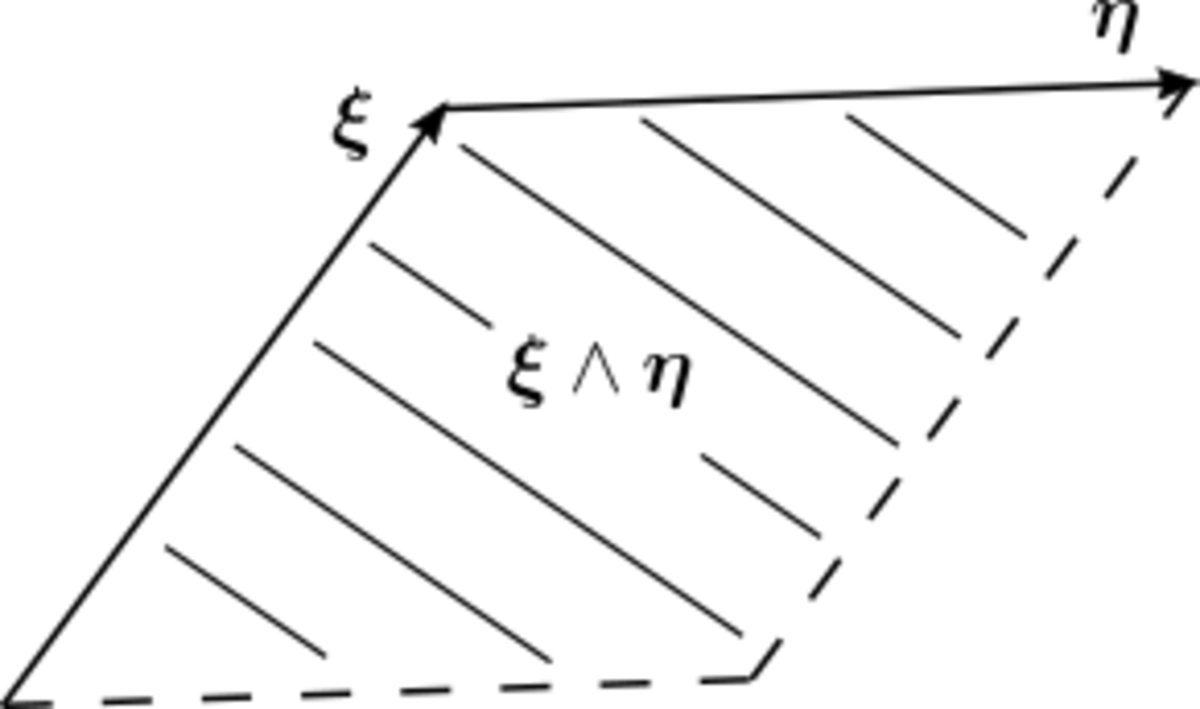
\includegraphics[width=.4\textwidth]{Imagens/paralelogramo.png}
    \centering
    \caption{Interpretação geométrica de $\boldsymbol{\xi}\wedge\boldsymbol{\eta}$}
    \label{a}
\end{figure}

Uma matriz $\mathbf{M}$ que preserva $\wedge$, isto é, que satisfaz
\begin{equation}
    \label{matrizes simpléticas 1}
    \mathbf{M}\boldsymbol{\xi}\wedge\mathbf{M}\boldsymbol{\eta} = \boldsymbol{\xi}\wedge\boldsymbol{\eta}
\end{equation}
para quaisquer $\boldsymbol{\xi}$ e $\boldsymbol{\eta}$, é dita simplética. Uma definição equivalente é exigir que $\mathbf{M}$ satisfaça
\begin{equation}
    \label{equação simplética}
    \mathbf{M}^T \mathbf{J} \mathbf{M} = \mathbf{J},
\end{equation}
onde o sobrescrito $T$ denota a transposição. Tomando o determinante de \eqref{equação simplética}, vemos que $\left| \det \mathbf{M} \right| = 1$, de forma que matrizes simpléticas são invertíveis. Além disso, multiplicando \eqref{equação simplética} por $\mathbf{M}^{-1}$ a direita e por $\left(\mathbf{M}^T\right)^{-1}$ a esquerda, obtemos
\begin{equation}
\label{fiquei com preguiça de dar nome}
    \left(\mathbf{M}^{-1}\right)^T \mathbf{J} \mathbf{M}^{-1} = \mathbf{J},
\end{equation}
isto é, $\mathbf{M}^{-1}$ também é simplética. Isso, junto com o fato de que o produto de duas matrizes simpléticas é simplética, o que pode ser deduzido de \eqref{equação simplética}, mostra que as matrizes simpléticas formam um grupo sob a operação de multiplicação. Notamos ainda que, tomando a inversa de ambos os lados de \eqref{fiquei com preguiça de dar nome}, obtemos 
\begin{equation}
    \label{equação simplética 2}
    \mathbf{M} \mathbf{J} \mathbf{M}^T = \mathbf{J},
\end{equation}
isto é, $\mathbf{M}^T$ também é simplética.

Considere a função $\boldsymbol{\Phi}:\mathbb{R}^{2d}\times\mathbb{R}\to \mathbb{R}^{2d}$; $(\mathbf{x},t) \mapsto \boldsymbol{\Phi}(\mathbf{x},t) = \boldsymbol{\Phi}_t(\mathbf{x})$ e que satisfaz
\begin{equation}
\label{definição fluxo hamiltoniano}
    \partial_t \boldsymbol{\Phi}(\mathbf{x},t) = \mathbf{J} \frac{\partial H}{\partial \mathbf{x}} \eval_{(\boldsymbol{\Phi}(\mathbf{x},t),t)} \ ; \ \ \ \boldsymbol{\Phi}(\mathbf{x},0) = \mathbf{x}
\end{equation}
isto é, $\boldsymbol{\Phi}(\mathbf{x},t)$ é obtido ao propagar $\mathbf{x}$, obedecendo as equações de Hamilton, por um tempo $t$. Diremos que $\boldsymbol{\Phi}$ é o fluxo hamiltoniano gerado pela hamiltoniana $H$.

Dada uma função $F:\mathbb{R}^{2d} \to \mathbb{R}^{2d}$, seja $\mathbf{y}(\mathbf{x},t) = F(\boldsymbol{\Phi}(\mathbf{x},t))$ \footnote{Observamos que, se quiséssemos o máximo de generalidade, o que não é o caso, deveríamos incluir uma dependência explicita de $F$ com o tempo.}. Diremos que a transformação $\mathbf{x} \mapsto \mathbf{y}$ é canônica se mantém as formas da equações de Hamilton \eqref{equações de hamilton}, isto é, se existe uma função $K(\mathbf{y},t)$ tal que
\begin{equation}
    \dot{\mathbf{y}} = \mathbf{J} \frac{\partial K}{\partial \mathbf{y}}
\end{equation}

\begin{lema}
\label{prop1}
    Se a matriz jacobiana $\partial \mathbf{y}/\partial \mathbf{x}$ é simplética, então a transformação $\mathbf{x} \mapsto \mathbf{y}$ é canônica.
\end{lema}
\begin{proof}
     Inserindo o jacobiano em \eqref{equação simplética 2}, obtemos
\begin{equation}
    \frac{\partial \mathbf{y}}{\partial \mathbf{x}} \mathbf{J} = \mathbf{J} \left(\frac{\partial \mathbf{x}}{\partial \mathbf{y}} \right)^T,
\end{equation}
e então,
\begin{equation}
    \dot{\mathbf{y}} = \frac{\partial \mathbf{y}}{\partial \mathbf{x}} \mathbf{J} \frac{\partial H}{\partial \mathbf{x}} = \mathbf{J} \left(\frac{d \mathbf{x}}{d \mathbf{y}} \right)^T \frac{\partial H}{\partial \mathbf{x}} = \mathbf{J} \frac{\partial}{\partial \mathbf{y}} H( \mathbf{x}\left(\mathbf{y}\right),t ),
\end{equation}
de onde identificamos $K(\mathbf{y},t) = H( \mathbf{x}\left(\mathbf{y}\right),t )$ como $H$ expressa em termos de $\mathbf{y}$.
\end{proof}

\begin{proposicao}
O fluxo hamiltoniano $\boldsymbol{\Phi}$ é uma transformação canônica.
\end{proposicao}

\begin{proof}
    Nesse caso, a função $F$ se reduz a identidade, de forma que, de acordo com o lema \ref{prop1}, é suficiente checar que $\partial \boldsymbol{\Phi}/ \partial \mathbf{x}$ é simplética para todo $t$. Em $t=0$, o jacobiano é a matriz identidade, devido à definição de $\boldsymbol{\Phi}$. Logo, se conseguirmos mostrar que
    \begin{equation}
    \label{derivada temporal da relação simpletica}
        \partial_t  \left[ \left( \frac{\partial\boldsymbol{\Phi}}{\partial \mathbf{x}} \right)^T \mathbf{J} \frac{\partial\boldsymbol{\Phi}}{\partial \mathbf{x}} \right] = 0,
    \end{equation}
    segue que
    \begin{equation}
        \left[ \left( \frac{\partial\boldsymbol{\Phi}}{\partial \mathbf{x}} \right)^T \mathbf{J} \frac{\partial\boldsymbol{\Phi}}{\partial \mathbf{x}} \right] \eval_{t=t_1} = \left[ \left( \frac{\partial\boldsymbol{\Phi}}{\partial \mathbf{x}} \right)^T \mathbf{J} \frac{\partial\boldsymbol{\Phi}}{\partial \mathbf{x}} \right] \eval_{t=0} = \mathbf{J},
    \end{equation}
    para um $t_1$ arbitrário, o que completaria a demonstração.
    
    Para demonstrar \eqref{derivada temporal da relação simpletica}, vemos que, de acordo com \eqref{definição fluxo hamiltoniano}, temos
    \begin{equation}
        \partial_t \frac{\partial\boldsymbol{\Phi}}{\partial \mathbf{x}} = \frac{\partial}{\partial \mathbf{x}} \partial_t\boldsymbol{\Phi} = \mathbf{J} \frac{\partial^2 H}{\partial \mathbf{x}^2} \frac{\partial\boldsymbol{\Phi}}{\partial \mathbf{x}}
    \end{equation}
    e, então,
    \begin{equation}
        \begin{aligned}
            \partial_t  \left[ \left( \frac{\partial\boldsymbol{\Phi}}{\partial \mathbf{x}} \right)^T \mathbf{J} \frac{\partial\boldsymbol{\Phi}}{\partial \mathbf{x}} \right] &=  \partial_t\left( \frac{\partial\boldsymbol{\Phi}}{\partial \mathbf{x}} \right)^T \mathbf{J} \frac{\partial\boldsymbol{\Phi}}{\partial \mathbf{x}} +  \left( \frac{\partial\boldsymbol{\Phi}}{\partial \mathbf{x}} \right)^T \mathbf{J} \partial_t\frac{\partial\boldsymbol{\Phi}}{\partial \mathbf{x}} \\ &= \left( \frac{\partial\boldsymbol{\Phi}}{\partial \mathbf{x}} \right)^T  \left( \frac{\partial^2 H}{\partial \mathbf{x}^2} \right)^T \mathbf{J}^T \mathbf{J} \frac{\partial\boldsymbol{\Phi}}{\partial \mathbf{x}} +  \left( \frac{\partial\boldsymbol{\Phi}}{\partial \mathbf{x}} \right)^T \mathbf{J} \mathbf{J} \frac{\partial^2 H}{\partial \mathbf{x}^2} \frac{\partial\boldsymbol{\Phi}}{\partial \mathbf{x}} = 0
        \end{aligned}
    \end{equation}
    sendo que, na última igualdade, utilizamos as relações \eqref{relações uteis J} e o fato de que a matriz hessiana $\partial^2 H/\partial \mathbf{x}^2$ é simétrica.
\end{proof}

\begin{exmp} 
\textit{Oscilador harmônico}

Com o objetivo de exemplificar a discussão anterior em um caso concreto, é instrutivo analisar o oscilador harmônico, com uma hamiltoniana $H(\mathbf{x}) = \omega \mathbf{x}^2/2$. Nesse caso, o fluxo é linear, e dado por $\boldsymbol{\Phi} \left( \mathbf{x},t \right) = \mathbf{M}_{\omega t} \mathbf{x}$, sendo
\begin{equation}
    \mathbf{M}_{\omega t} = \begin{pmatrix} \cos \omega t & -\sin \omega t \\ \sin \omega t & \cos \omega t,
    \end{pmatrix}
\end{equation}
uma matriz de rotação. O jacobiano $\partial \boldsymbol{\Phi}/\partial \mathbf{x}$ coincide então com $\mathbf{M}_{\omega t}$, que, por um cálculo direto, prova-se constituir uma matriz simplética. Em particular, temos $\boldsymbol{\Phi} \left( \mathbf{x}, \pi/\omega \right) = -\mathbf{x}$, isto é, o fluxo se reduz a uma reflexão com centro na origem.

\end{exmp}
\begin{exmp}
\textit{Reflexões e Translações}

Definimos uma reflexão $R_\mathbf{\mathbf{x}}$ em torno de um centro $\mathbf{x}$ de forma que valha $R_{\mathbf{x}}\left( \mathbf{x}_- \right) - \mathbf{x} = - \left( \mathbf{x}_- - \mathbf{x}\right)$, ou, explicitamente, $R_{\mathbf{x}}\left( \mathbf{x}_- \right) = 2 \mathbf{x} - \mathbf{x}_-$ como na figura \ref{reflexão}. Checa-se que essa classe de transformações é canônica, uma vez que seu jacobiano é $-\mathbf{I}$. Uma outra classe de transformações canônicas é dada pelas translações $T_{\boldsymbol{\xi}}\left( \mathbf{x}_- \right) = \mathbf{x}_- + \boldsymbol{\xi}$ por uma corda $\boldsymbol{\xi}$, que, desta vez, possuem jacobiano $\mathbf{I}$. Junto com as reflexões, essas transformações formam um grupo sob a operação de composição, uma vez que valem as relações

\begin{subequations}
\label{reflexões e translações clássicas}
    \begin{equation}
        T_{\boldsymbol{\xi}_2}\circ T_{\boldsymbol{\xi}_1} = T_{\boldsymbol{\xi}_1+\boldsymbol{\xi}_2}
    \end{equation}
    \begin{equation}
         R_\mathbf{x}\circ T_{\boldsymbol{\xi}}=  R_{\mathbf{x}-\boldsymbol{\xi}/2}
    \end{equation}
    \begin{equation}
        T_{\boldsymbol{\xi}}\circ R_\mathbf{x} =  R_{\mathbf{x}+\boldsymbol{\xi}/2}
    \end{equation}
    \begin{equation}
        R_{\mathbf{x}_2} \circ R_{\mathbf{x}_1} =  T_{2(\mathbf{x}_2-\mathbf{x}_1)}
    \end{equation}
\end{subequations}
Esse grupo e suas propriedades serão de fundamental importância ao longo deste trabalho.

\begin{figure}[H]
     \centering
     \begin{subfigure}[b]{0.3\textwidth}
         \centering
         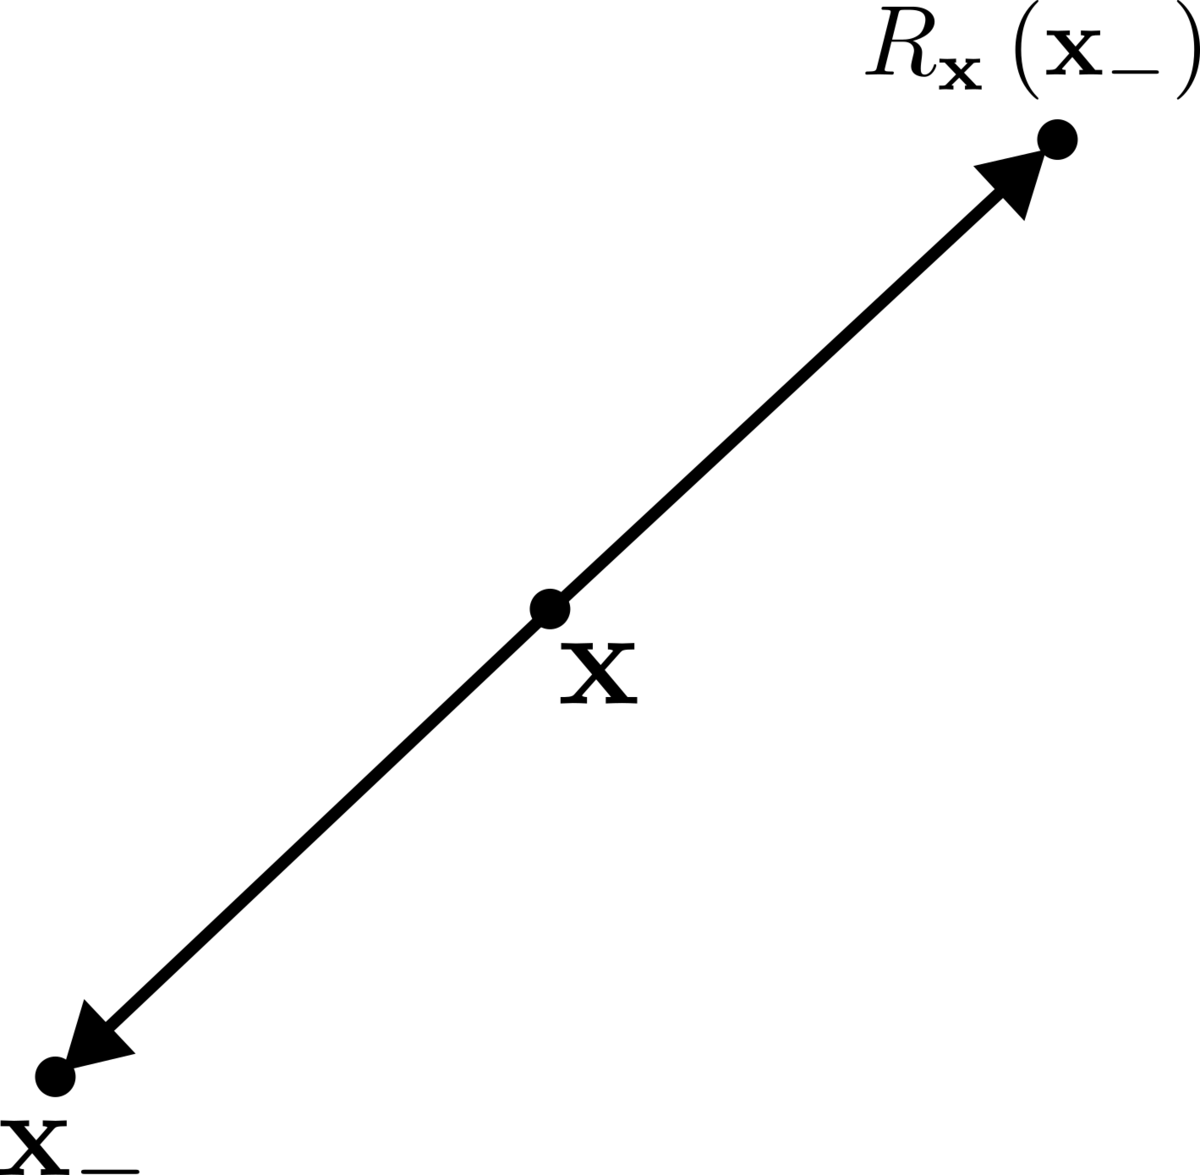
\includegraphics[width=\textwidth]{Imagens/reflexão.png}
         \caption{Reflexão}
         \label{reflexão}
     \end{subfigure}
     ~ ~ ~ ~~~~~~~~
     \begin{subfigure}[b]{0.3\textwidth}
         \centering
         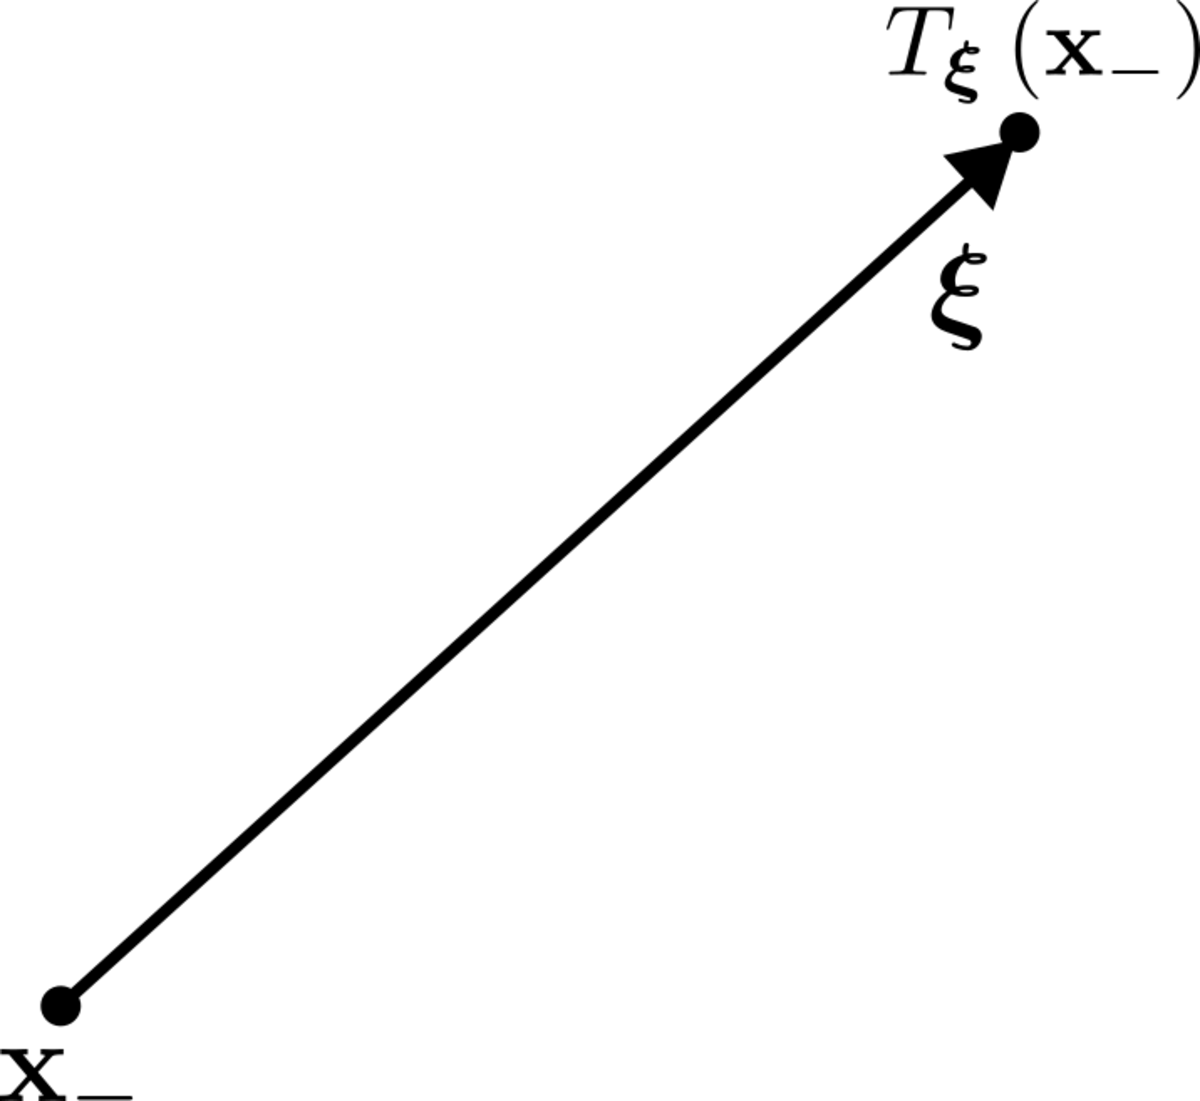
\includegraphics[width=\textwidth]{Imagens/translação.png}
         \caption{Translação}
         \label{translação}
     \end{subfigure}
        \label{reflexão e translação}
\end{figure}

\end{exmp}

\section{Funções Geratrizes de Centros}
\label{funções geratrizes}

Considere uma certa transformação $\mathbf{x}_- \mapsto \mathbf{x}_+$. Definimos a corda $\boldsymbol{\xi}$ e o centro $\mathbf{x}$ desta transformação por
\begin{equation}
    \begin{cases}
        \boldsymbol{\xi} = \mathbf{x}_+ - \mathbf{x}_- \\
        \mathbf{x} = \dfrac{\mathbf{x}_++\mathbf{x}_-}{2}
    \end{cases} \Leftrightarrow \mathbf{x}_\pm = \mathbf{x} \pm \frac{1}{2}\boldsymbol{\xi}
\end{equation}
e, se fornecermos a corda $\boldsymbol{\xi}(\mathbf{x})$ correspondente a cada centro $\mathbf{x}$, caracterizamos completamente a transformação. Em particular, dada uma função arbitrária $S$, podemos definir $\boldsymbol{\xi}(\mathbf{x})$ por
\begin{equation}
    \boldsymbol{\xi}(\mathbf{x}) = -\mathbf{J} \frac{\partial S}{\partial \mathbf{x}}
\end{equation}
e a transformação correspondente é canônica. De fato, temos
\begin{equation}
    \frac{\partial \mathbf{x}_{\pm}}{ \partial \mathbf{x}} = \mathbf{I} \mp \frac{\mathbf{J}}{2} \frac{\partial^2 S}{\partial \mathbf{x}^2},
\end{equation}
e, então
\begin{equation}
\label{jacobiano transformação canônica de centro}
    \frac{\partial \mathbf{x}_+}{ \partial \mathbf{x}_-} = \frac{\partial \mathbf{x}_+}{ \partial \mathbf{x}} \frac{\partial \mathbf{x}}{ \partial \mathbf{x}_-} = \left(\mathbf{I} - \frac{\mathbf{J}}{2} \frac{\partial^2 S}{\partial \mathbf{x}^2}\right) \left(\mathbf{I} + \frac{\mathbf{J}}{2} \frac{\partial^2 S}{\partial \mathbf{x}^2}\right)^{-1}.
\end{equation}
Checa-se por um cálculo direto que o jacobiano dado por esta expressão satisfaz \eqref{equação simplética}, sendo necessário apenas utilizar o fato de que a hessiana $\partial^2 S/\partial \mathbf{x}^2$ é uma matriz simétrica. Nesse contexto, nos referimos a $S$ como a função geratriz de centros. Vemos imediatamente que, se duas funções geratrizes diferem por uma quantidade independente de $\mathbf{x}$, então geram a mesma transformação. 

Quando a transformação canônica em questão é o fluxo hamiltoniano, também nos referiremos a $S$ por ação. Tendo em vista que
\begin{equation}
    \dot{\mathbf{x}} = \mathbf{J} \frac{\partial H}{\partial \mathbf{x}} \Rightarrow \mathbf{x}(t) - \mathbf{x}(0) = t\mathbf{J} \frac{\partial H}{\partial \mathbf{x}} + \order{t^2},
\end{equation}
vemos que a corda correspondente ao fluxo hamiltoniano pode ser escrita como
\begin{equation}
    \boldsymbol{\xi} = t\mathbf{J} \frac{\partial H}{\partial \mathbf{x}} + \order{t^3},
\end{equation}
sendo a primeira correção de ordem $3$ no tempo pois $t \mapsto -t \Rightarrow \boldsymbol{\xi} \mapsto -\boldsymbol{\xi}$. Assim sendo, a ação deve satisfazer
\begin{equation}
\label{ação primeira ordem}
    S(\mathbf{x},t) = S_t(\mathbf{x}) = -tH(\mathbf{x}) + \order{t^3}.
\end{equation}

\begin{exmp}
    Considere uma função geratriz da forma
    \begin{equation}
        S(\mathbf{x}) =  \mathbf{x} \cdot \mathbf{B}\mathbf{x}
    \end{equation}
    onde $\mathbf{B}$, sem perda de generalidade, pode ser tomado como uma matriz simétrica. Temos então
    \begin{equation}
        \mathbf{x}_+ - \mathbf{x}_- = \boldsymbol{\xi} = -\mathbf{J} \frac{\partial S}{\partial \mathbf{x}} = -2\mathbf{J}\mathbf{B}\mathbf{x} = -\mathbf{J} \left(\mathbf{x}_+ + \mathbf{x}_-\right),
    \end{equation}
    e, portanto,
    \begin{equation}
        \label{transf_ação_quadratica}
        \mathbf{x}_+ = \left(\mathbf{I} + \mathbf{J}\mathbf{B}\right)^{-1}\left(\mathbf{I} - \mathbf{J}\mathbf{B}\right)\mathbf{x}_-,
    \end{equation}
    isto é, obtemos uma transformação linear.

    Para hamiltonianas da forma
    \begin{equation}
        H(\mathbf{x}) = \frac{1}{2} \mathbf{x} \cdot \boldsymbol{\mathcal{H}}_{\mathbf{0}} \mathbf{x}
    \end{equation}
    o fluxo é dado simplesmente por
    \begin{equation}
    \label{fluxo linear}
        \mathbf{x}(t) = \mathbf{M}_t \mathbf{x}(0), \ \ \ \mathbf{M}_t = \exp(t \mathbf{J} \boldsymbol{\mathcal{H}}_{\mathbf{0}})
    \end{equation}
    e, comparando este resultado com \eqref{transf_ação_quadratica}, temos
    \begin{equation}
        \left(\mathbf{I} + \mathbf{J}\mathbf{B}\right)^{-1}\left(\mathbf{I} - \mathbf{J}\mathbf{B}\right) = \mathbf{M}_t
    \end{equation}
    e, então
    \begin{equation}
        \begin{aligned}
            \boldsymbol{B} &= -\mathbf{J} (\mathbf{I}+\mathbf{M}_t)^{-1}(\mathbf{I}-\mathbf{M}_t) \\
            &= \mathbf{J}\tanh \left(\frac{t}{2}\mathbf{J} \boldsymbol{\mathcal{H}}_{\mathbf{0}}\right) \\
        \end{aligned}
    \end{equation}
\end{exmp}

\begin{exmp}
    Considere agora uma função geratriz da forma
    \begin{equation}
        S(\mathbf{x}) = \mathbf{x} \cdot \mathbf{a} + \mathbf{x} \cdot \mathbf{B}\mathbf{x}
    \end{equation}
    sendo $\mathbf{a}$ um vetor e $\mathbf{B}$ uma matriz simétrica. Desta vez, temos
    \begin{equation}
        \mathbf{x}_+ - \mathbf{x}_- = \boldsymbol{\xi} = -\mathbf{J} \frac{\partial S}{\partial \mathbf{x}} = -\mathbf{J} \mathbf{a}  -\mathbf{J} \left(\mathbf{x}_+ + \mathbf{x}_-\right),
    \end{equation}
    e, portanto,
    \begin{equation}
        \mathbf{x}_+ = -\left(\mathbf{I} + \mathbf{J}\mathbf{B}\right)^{-1} \mathbf{J} \mathbf{a} + \left(\mathbf{I} + \mathbf{J}\mathbf{B}\right)^{-1}\left(\mathbf{I} - \mathbf{J}\mathbf{B}\right)\mathbf{x}_-,
    \end{equation}
    isto é, obtemos uma transformação afim.

    Para hamiltonianas da forma
    \begin{equation}
        \label{hamiltoniana_quadrática}
        H(\mathbf{x}) = \mathbf{x} \cdot \mathbf{h}_{\mathbf{0}} + \frac{1}{2} \mathbf{x} \cdot \boldsymbol{\mathcal{H}}_{\mathbf{0}} \mathbf{x}
    \end{equation}
    o fluxo é 
    \begin{equation}
        \mathbf{x}(t) = \mathbf{M}_t \left[\mathbf{x}(0) + \boldsymbol{\mathcal{H}}^{-1}_{\mathbf{0}} \mathbf{h}_{\mathbf{0}} \right] -  \boldsymbol{\mathcal{H}}^{-1}_{\mathbf{0}}\mathbf{h}_{\mathbf{0}}
    \end{equation}
    de forma que identificamos
    \begin{equation}
        \begin{aligned}
            \mathbf{B} = \mathbf{J}\tanh \left(\frac{t}{2}\mathbf{J} \boldsymbol{\mathcal{H}}_{\mathbf{0}}\right) ;
        \end{aligned}
    \end{equation}
    \begin{equation}
        \mathbf{a} =  2\mathbf{J}\tanh \left(\frac{t}{2}\mathbf{J} \boldsymbol{\mathcal{H}}_{\mathbf{0}}\right) \boldsymbol{\mathcal{H}}_{\mathbf{0}}^{-1} \mathbf{h_0}
    \end{equation}
    sendo então a ação dada por
    \begin{equation}
    \label{ação quadratica multidimensional}
        S(\mathbf{x},t) = \mathbf{x} \cdot \mathbf{J}\tanh \left(\frac{t}{2}\mathbf{J} \boldsymbol{\mathcal{H}}_{\mathbf{0}}\right)\left(  2 \boldsymbol{\mathcal{H}_{\mathbf{0}}}^{-1} \mathbf{h_0} +  \mathbf{x}\right)
    \end{equation}
    Para um grau de liberdade, podemos simplificar ainda mais essa fórmula. Para isso, lembramos que a adjunta clássica $\text{adj }  \mathbf{A}$ de uma matriz quadrada $\mathbf{A}$ é também uma matriz quadrada \cite{lima2016algebra}, que satisfaz
    \begin{equation}
    \label{definição adjunta}
        \mathbf{A} \ \text{adj } \mathbf{A} = \left( \det \mathbf{A} \right) \ \mathbf{I}
    \end{equation}
    No caso em que
    \begin{equation}
        \mathbf{A} = \begin{pmatrix}
        a & b \\
        c & d
        \end{pmatrix},
    \end{equation}
    temos
    \begin{equation}
        \text{adj } \mathbf{A} = \begin{pmatrix}
        d & -b \\
        -c & a
        \end{pmatrix}.
    \end{equation}
    Além disso, se $\mathbf{A}$ for simétrica, como ocorre para hessianas, mostra-se por um cálculo direto que, no caso $2 \times 2$, vale
    \begin{equation}
        \text{adj } \mathbf{A} = -\mathbf{J} \mathbf{A} \mathbf{J},
    \end{equation}
    relação esta que, combinada com $\eqref{definição adjunta}$, nos fornece $\left(\boldsymbol{\mathcal{H}}_\mathbf{0} \mathbf{J}\right)^2 = \left(\mathbf{J}\boldsymbol{\mathcal{H}}_\mathbf{0} \right)^2 = -\Omega^2 \mathbf{I}$, $\Omega^2 = \det \boldsymbol{\mathcal{H}}_\mathbf{0}$. Substituindo esta expressão em \eqref{ação quadratica multidimensional}, obtemos
    \begin{equation}
    \label{ação_quadŕatica}
        \begin{aligned}
            S(\mathbf{x},t) &= -\frac{2}{\Omega}\tan \left(\frac{\Omega t}{2}\right) \left(  \mathbf{x} \cdot \mathbf{h_0} +  \frac{1}{2}\mathbf{x} \cdot \boldsymbol{\mathcal{H}_{\mathbf{0}}} \mathbf{x}\right) \\
            &= -\frac{2}{\Omega}\tan \left(\frac{\Omega t}{2}\right) H(\mathbf{x}).
        \end{aligned}
    \end{equation}
    Observamos que, quando $\Omega t = (2n+1) \pi$, para qualquer $n \in \mathbb{Z}$, esta expressão se torna divergente. Esse fenômeno será discutido em mais detalhes na seção \ref{Cáusticas e outras funções geratrizes}.
\end{exmp}

\section{Ação para sistemas arbitrários}
\label{composição funções geratrizes}

Como veremos ao longo desse trabalho, será de extrema importância a obtenção da ação para um sistema arbitrário e, nesta seção, desenvolveremos as técnicas necessárias para este cálculo. Primeiramente, discutiremos uma aproximação que gera uma expressão analítica e, em seguida, deduziremos uma fórmula exata, mas que, em geral, só pode ser calculada numericamente.

\subsection{Expressão Aproximada}
\label{Expressões Aproximadas}

O desenvolvimento de aproximações para a ação nos será útil pois permite a obtenção de expressões analíticas cujo custo computacional é muito menor quando comparados a fórmula exata. A que discutiremos aqui é obtida a partir da observação de que, em torno de cada ponto $\mathbf{x}$ no espaço de fase, podemos aproximar o fluxo gerado por uma hamiltoniana arbitrária por aquele gerado pelo polinômio de Taylor de segunda ordem desta hamiltoniana. Nossa ideia é então manipular \eqref{ação_quadŕatica}, que é a expressão exata da ação para esse tipo de sistema, e escrevê-la em termos da hamiltoniana \eqref{hamiltoniana_quadrática}, de seu gradiente $\mathbf{h}_\mathbf{x} = \mathbf{h}_{\mathbf{0}} + \boldsymbol{\mathcal{H}}_{\mathbf{0}} \mathbf{x}$ e de sua hessiana $\boldsymbol{\mathcal{H}}_\mathbf{x} = \boldsymbol{\mathcal{H}}_{\mathbf{0}}$. Começamos reescrevendo \eqref{ação_quadŕatica} como
\begin{equation}
\label{expressão_aa}
    S(\mathbf{x},t) = -t H(\mathbf{x}) +  \left[t-\frac{2}{\Omega}\tan \left(\frac{\Omega t}{2}\right)\right] H(\mathbf{x}),
\end{equation}
de forma que o primeiro termo já é correto em $\order{t}$ para hamiltonianas arbitrárias. Agora, observamos que, quando $\boldsymbol{\mathcal{H}}_\mathbf{x}$ é invertível, podemos escrever
\begin{equation}
        \begin{aligned}
        H(\mathbf{x}) &= \frac{1}{2} \boldsymbol{\mathcal{H}}_\mathbf{x}^{-1}\left(\mathbf{h}_\mathbf{x}-\mathbf{h}_{\mathbf{0}}\right) \cdot \left(\mathbf{h}_\mathbf{x} + \mathbf{h}_{\mathbf{0}}\right) \\
        &= \frac{1}{2} \boldsymbol{\mathcal{H}}_\mathbf{x}^{-1}\mathbf{h}_\mathbf{x} \cdot \mathbf{h}_\mathbf{x}  - \frac{1}{2} \boldsymbol{\mathcal{H}}_\mathbf{x}^{-1}\mathbf{h}_\mathbf{0} \cdot \mathbf{h}_\mathbf{0}
    \end{aligned}
\end{equation}
Expressando a hamiltoniana no segundo termo de \eqref{expressão_aa} por esta fórmula, omitindo o termo proporcional a $\boldsymbol{\mathcal{H}}_\mathbf{x}^{-1}\mathbf{h}_\mathbf{0} \cdot \mathbf{h}_\mathbf{0}$, que é uma constante, e substituindo $\Omega$ por $\Omega_\mathbf{x} = \sqrt{\det \boldsymbol{\mathcal{H}}_\mathbf{x}}$, obtemos
\begin{equation}
\label{metapletica_amortecida_real}
    \begin{aligned}
        S(\mathbf{x},t) &= -t H(\mathbf{x}) + \left[\frac{t}{2}-\frac{1}{\Omega_\mathbf{x}}\tan \left(\frac{\Omega_\mathbf{x} t}{2}\right)\right] \boldsymbol{\mathcal{H}}_\mathbf{x}^{-1}\mathbf{h}_\mathbf{x} \cdot \mathbf{h}_\mathbf{x} \\
        &= -t H(\mathbf{x}) + \frac{1}{\Omega_\mathbf{x}^2}\left[\frac{t}{2}-\frac{1}{\Omega_\mathbf{x}}\tan \left(\frac{\Omega_\mathbf{x} t}{2}\right)\right] \left( \text{adj } \boldsymbol{\mathcal{H}}_\mathbf{x} \right) \mathbf{h}_\mathbf{x} \cdot \mathbf{h}_\mathbf{x}
    \end{aligned}
\end{equation}
Esta última expressão, obtida em \cite{OZORIODEALMEIDA2021132951}, é exata para hamiltonianas quadráticas, uma vez que foi deduzida de \eqref{ação_quadŕatica} através do uso de identidades, mas, quando avaliada para hamiltonianas arbitrárias, pode ser interpretada como uma aproximação cuja validade será avaliada ao longo deste trabalho. Observamos ainda que, ao expandir $\tan$ em uma série de potências, é possível checar que essa aproximação possui um limite bem definido mesmo quando $\Omega_{\mathbf{x}} \to 0$, isto é, quando $\boldsymbol{\mathcal{H}}_\mathbf{x}$ deixa de ser invertível.

\subsection{Expressão Exata}

Para a obtenção da expressão exata da ação, o ponto de partida é a observação de que o fluxo $\boldsymbol{\Phi}_t$ correspondente a um tempo $t$ pode ser escrito como a composição de $N$ fluxos de tempo $t/N$, isto é, $\boldsymbol{\Phi}_t = \boldsymbol{\Phi}_{t/N} \circ \cdots \circ \boldsymbol{\Phi}_{t/N}$. A estratégia é então utilizar a expressão \eqref{ação primeira ordem} para escrever a ação correspondente aos tempos curtos $t/N$, compô-las de forma a construir a ação para o tempo $t$, e, por fim, tomar $N \to \infty$.

A etapa mais complicada de nossa estratégia é a composição das ações, ou mais geralmente, a composição de funções geratrizes. Para elucidar essa questão, primeiramente focamos no caso da composição de duas funções geratrizes $S_1$ e $S_2$, que geram respectivamente as transformações $T_1$ e $T_2$. Queremos obter então a função geratriz $S$ correspondente à transformação $T = T_2 \circ T_1$. Para fazer isso, é conveniente analisar o triângulo cujos vértices são os pontos $\mathbf{x}_-,T_1\left(\mathbf{x}_-\right),T\left(\mathbf{x}_-\right)$, para algum $\mathbf{x}_-$ arbitrário, como mostrado na figura \ref{composição_duas_transformações}. Vemos então que os lados são dados pelas cordas $\boldsymbol{\xi},\boldsymbol{\xi}_1,\boldsymbol{\xi}_2$ correspondentes às transformações $T,T_1$ e $T_2$, além de estarem centrados nos pontos $\mathbf{x},\mathbf{x}_1,\mathbf{x}_2$. 

\begin{figure}[H]
    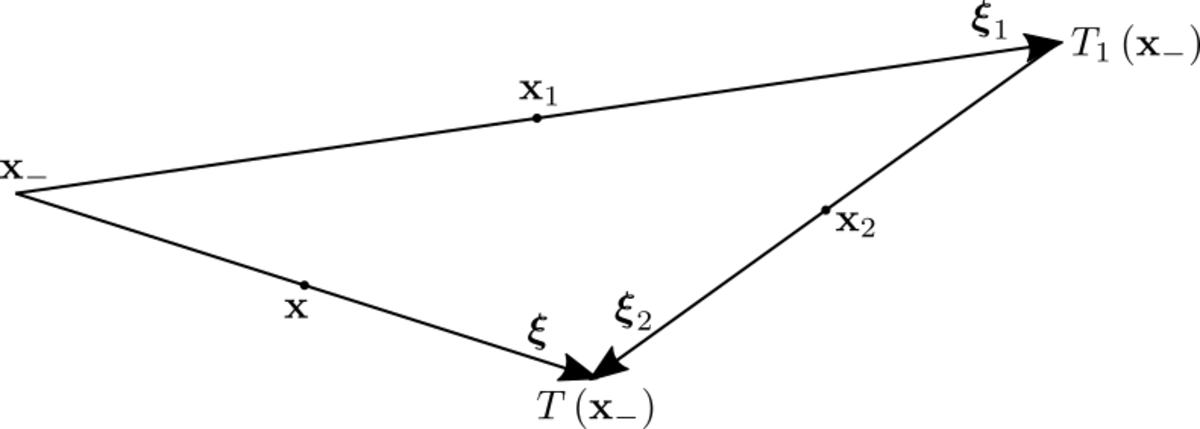
\includegraphics[width=.8\textwidth]{Imagens/triangles.png}
    \centering
    \caption{Geometria da composição de duas transformações}
    \label{composição_duas_transformações}
\end{figure}

Da simples geometria do problema, podemos obter as relações
\begin{subequations}
    \begin{equation}
        \mathbf{x}_2 - \mathbf{x}_1 = \frac{1}{2}\boldsymbol{\xi}
    \end{equation}
    \begin{equation}
        \mathbf{x}_2 - \mathbf{x} = \frac{1}{2}\boldsymbol{\xi}_1
    \end{equation}
    \begin{equation}
        \mathbf{x} - \mathbf{x}_1 = \frac{1}{2}\boldsymbol{\xi}_2
    \end{equation}
\end{subequations}
e, utilizando-as, podemos escrever a área $\boldsymbol{\xi}_1 \wedge \boldsymbol{\xi}_2/2$ do triângulo como 
\begin{equation}
    \begin{aligned}
        \Delta_3 (\mathbf{x},\mathbf{x}_1,\mathbf{x}_2) &= 2 \left( \mathbf{x}_1 - \mathbf{x} \right) \wedge \left( \mathbf{x}_2 - \mathbf{x} \right) \\
        &= 2 \left( \mathbf{x} \wedge \mathbf{x}_1 + \mathbf{x}_1 \wedge \mathbf{x}_2 + \mathbf{x}_2 \wedge \mathbf{x} \right)
    \end{aligned}
\end{equation}
Notamos ainda que
\begin{subequations}
    \begin{equation}
        \frac{\partial \Delta_3}{\partial \mathbf{x}_1} = - 2 \mathbf{J} \left( \mathbf{x}_2 - \mathbf{x} \right) = -\mathbf{J} \boldsymbol{\xi}_1 
    \end{equation}
    \begin{equation}
        \frac{\partial \Delta_3}{\partial \mathbf{x}_2} =  2 \mathbf{J} \left( \mathbf{x}_1 - \mathbf{x} \right) = -\mathbf{J} \boldsymbol{\xi}_2,
    \end{equation}
\end{subequations}
equações estas que, utilizando o fato de que $T_i$ é gerada por $S_i$, isto é, $\boldsymbol{\xi}_i = -\mathbf{J} d S_i /d \mathbf{x}_i$, podem ser reescritas como
\begin{subequations}
    \begin{equation}
        \frac{\partial \Delta_3}{\partial \mathbf{x}_1} = - \frac{d S_1}{d \mathbf{x}_1}
    \end{equation}
    \begin{equation}
        \frac{\partial \Delta_3}{\partial \mathbf{x}_2} =  - \frac{d S_2}{d \mathbf{x}_2}
    \end{equation}
\end{subequations}
ou, ainda,
\begin{subequations}
    \label{derivadas_se_anulam}
    \begin{equation}
        \frac{\partial F}{\partial \mathbf{x}_1} = 0
    \end{equation}
    \begin{equation}
        \frac{\partial F}{\partial \mathbf{x}_2} = 0
    \end{equation}
\end{subequations}
onde $F$ é a função definida por
\begin{equation}
    F(\mathbf{x},\mathbf{x}_1,\mathbf{x}_2) = S_1\left(\mathbf{x}_1\right) + S_2\left(\mathbf{x}_2\right) + \Delta_3 (\mathbf{x},\mathbf{x}_1,\mathbf{x}_2).
\end{equation}
Denotando por $\mathbf{x}_1 \left( \mathbf{x} \right)$ e $\mathbf{x}_2 \left( \mathbf{x} \right)$ as soluções do sistema de equações \eqref{derivadas_se_anulam}, afirmamos que a função geratriz de $T$ é dada então por $S(\mathbf{x}) = F\left[\mathbf{x},\mathbf{x}_1 \left(\mathbf{x}\right),\mathbf{x}_2 \left(\mathbf{x}\right)\right]$. De fato,
\begin{equation}
    \begin{aligned}
        \frac{d S}{d \mathbf{x}} &= \frac{\partial F}{\partial \mathbf{x}} \eval_{\left[ \mathbf{x}, \mathbf{x}_1 \left(\mathbf{x}\right),\mathbf{x}_2 \left(\mathbf{x}\right)\right] }  \\ &= \frac{\partial \Delta_3}{\partial \mathbf{x}} \eval_{\left[ \mathbf{x}, \mathbf{x}_1 \left(\mathbf{x}\right),\mathbf{x}_2 \left(\mathbf{x}\right)\right] } \\ &= 2 \mathbf{J} \left[ \mathbf{x}_2 \left(\mathbf{x}\right) - \mathbf{x}_1 \left(\mathbf{x}\right) \right] = \mathbf{J} \boldsymbol{\xi}
    \end{aligned}
\end{equation}

Para generalizar esse resultado para a composição de $N$ transformações, precisamos achar uma função $\Delta_{N+1}\left(\mathbf{x},\mathbf{x}_1,\ldots,\mathbf{x}_N\right)$ que satisfaça
\begin{equation}
    \frac{\partial \Delta_{N+1}}{\partial \mathbf{x}_j} = - \mathbf{J} \boldsymbol{\xi}_j, \ \ \ j = 1,\ldots,N; \ \ \ \ \frac{\partial \Delta_{N+1}}{\partial \mathbf{x}} = \mathbf{J} \boldsymbol{\xi}.
\end{equation}
Desta forma, sendo
\begin{equation}
    F(\mathbf{x},\mathbf{x}_1,\ldots,\mathbf{x}_N) = S_1\left(\mathbf{x}_1\right) + \cdots +  S_N \left(\mathbf{x}_N\right) + \Delta_{N+1}\left(\mathbf{x},\mathbf{x}_1,\ldots,\mathbf{x}_N\right)
\end{equation}
e $\mathbf{x}_1\left(\mathbf{x}\right), \ldots, \mathbf{x}_N\left(\mathbf{x}\right)$ a solução do sistema
\begin{equation}
    \label{limite_estacionario}
    \frac{\partial F}{\partial \mathbf{x}_j} \eval_{\mathbf{x},\mathbf{x}_1\left(\mathbf{x}\right), \ldots, \mathbf{x}_N\left(\mathbf{x}\right)} = 0, \ \ \ j = 1,\ldots,N
\end{equation}
temos $S(\mathbf{x}) = F \left[\mathbf{x},\mathbf{x}_1\left(\mathbf{x}\right), \ldots, \mathbf{x}_N\left(\mathbf{x}\right)\right]$, uma vez que
\begin{equation}
    \begin{aligned}
        \frac{d S}{d \mathbf{x}} &= \frac{\partial F}{\partial \mathbf{x}} \eval_{\mathbf{x},\mathbf{x}_1\left(\mathbf{x}\right), \ldots, \mathbf{x}_N\left(\mathbf{x}\right)}  \\ &= \frac{\partial \Delta_{N+1}}{\partial \mathbf{x}}\eval_{\mathbf{x},\mathbf{x}_1\left(\mathbf{x}\right), \ldots, \mathbf{x}_N\left(\mathbf{x}\right)} =  \mathbf{J} \boldsymbol{\xi}
    \end{aligned}
\end{equation}

É mostrado no apêndice \ref{apendice_area} que, quando $N$ é par, $\Delta_{N+1}$ continua sendo a área do polígono cujos $N+1$ lados estão centrados em $\mathbf{x},\mathbf{x}_1, \ldots, \mathbf{x}_N$, de modo que já temos todos os elementos para prosseguir na nossa estratégia para a obtenção da ação. Escrevendo $S_t$ em termos de $S_{t/N}$ e utilizando \eqref{ação primeira ordem}, obtemos
\begin{equation}
    \begin{aligned}
        S(\mathbf{x},t) &= \sum_{j=1}^N S(\mathbf{x}_j,t/N) + \Delta_{N+1}\left(\mathbf{x},\mathbf{x}_1,\ldots,\mathbf{x}_n\right) \\
        &=-\frac{t}{N}\sum_{j=1}^N H\left(\mathbf{x}_j\right) + \Delta_{N+1}\left(\mathbf{x},\mathbf{x}_1,\ldots,\mathbf{x}_N\right) + \order{t^3/N^2} .
    \end{aligned}
\end{equation}
Quando aumentamos $N$, o termo $\order{t^3/N^2}$ se torna cada vez menor e o polígono com lados centrados em $\mathbf{x},\mathbf{x}_1,\ldots,\mathbf{x}_N$ se aproxima da região entre a trajetória e a corda, cuja área denotamos por $\Delta$. Esse processo é ilustrado na figura \ref{aproximação_trajetória_poligonos}. No limite $N\to \infty$, obtemos, finalmente,
\begin{equation}
\label{ação}
    S(\mathbf{x},t) = \Delta - \int H \left[\mathbf{x}(t)\right] dt. 
\end{equation}
Além disso, as equações \eqref{limite_estacionario}, que são mantidas ao tomar o limite, nos permitem obter o princípio variacional de centros: \textit{de todas as curvas que compartilham o mesmo centro, a evolução temporal é um extremo da ação.}

\begin{figure}[H]
    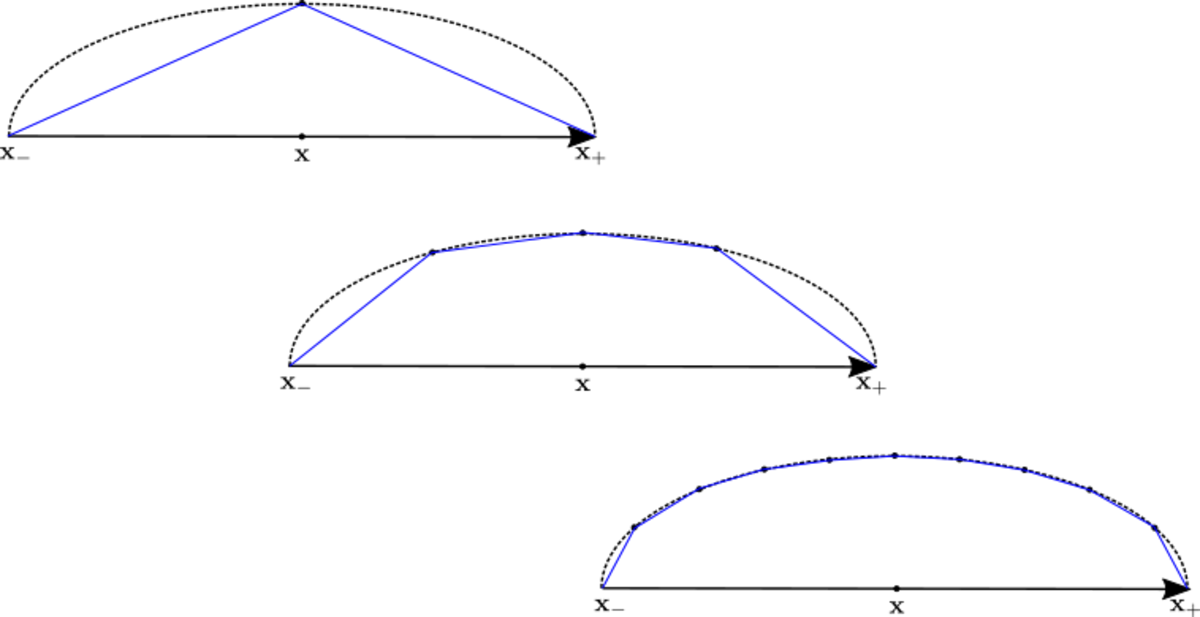
\includegraphics[width=\textwidth]{Imagens/trajetóriav2.png}
    \centering
    \caption{Sequência de aproximações da trajetória (tracejada) por polígonos (azul).}
    \label{aproximação_trajetória_poligonos}
\end{figure}

A expressão \eqref{ação} ainda não é muito conveniente para cálculos explícitos, uma vez que a trajetória relevante fica apenas implicitamente definida a partir do centro da trajetória $\mathbf{x}$. Para remediar esse problema, é conveniente prosseguir da seguinte forma — consideramos que, a partir de um ponto inicial $\mathbf{X}$, evoluímos duas trajetórias, uma na direção usual do tempo e a outra para a trás, isto é, resolvemos as equações
\begin{equation}
\label{não sei dar nomeee}
   \dot{\mathbf{x}}_{\pm} = \pm \mathbf{J} \frac{\partial H}{\partial \mathbf{x}} \eval_{ \mathbf{x}_{\pm} }, \ \ \ \mathbf{x}_{\pm} \left( t = 0 \right) = \mathbf{X}.
\end{equation}
Definindo
\begin{equation}
\label{problema valor inicial}
    \mathbf{x}(\mathbf{X},t) = \frac{\mathbf{x}_{+}(t)+\mathbf{x}_{-}(t)}{2}, \ \ \ \boldsymbol{\xi}(\mathbf{X},t) = \mathbf{x}_{+}(t)-\mathbf{x}_{-}(t)
\end{equation}
vemos que $\mathbf{x}\left( \mathbf{X},t/2\right)$ é o centro de uma trajetória que parte de $\mathbf{x}_{-}(t/2)$, e, depois de um tempo $t$, chega a $\mathbf{x}_{+}(t/2)$, enquanto $\boldsymbol{\xi}\left( \mathbf{X},t/2\right)$ é a corda correspondente, como na figura \eqref{meia trajetória}. Diremos ainda que $\mathbf{X}$ é o ponto médio da trajetória.

\begin{figure}[H]
    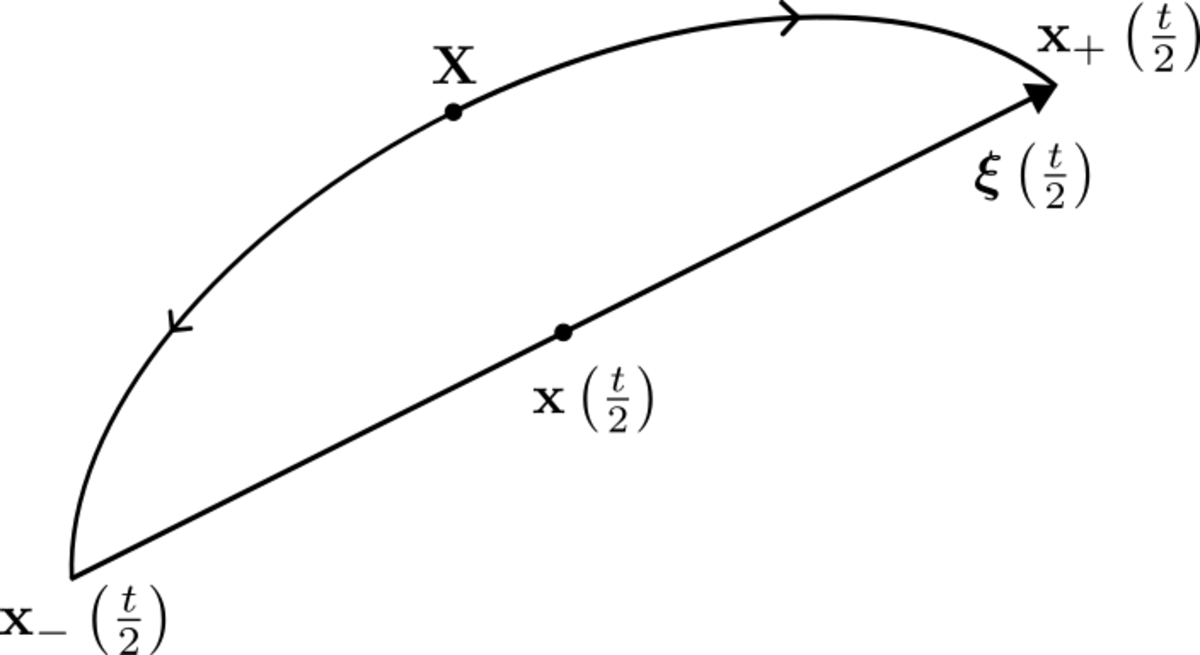
\includegraphics[width=0.6\textwidth]{Imagens/half_trajectories.png}
    \centering
    \caption{Trajetória especificada a partir de seu ponto médio $\mathbf{X}$.}
    \label{meia trajetória}
\end{figure}

Esta construção é útil pois, como mostramos no apêndice \ref{Cálculo do termo de área}, uma vez obtidos $\mathbf{x}$ e $\boldsymbol{\xi}$, podemos calcular a área entre a corda e a trajetória através da expressão
\begin{equation}
    \Delta\left[ \mathbf{x}\left( \mathbf{X}\right),t \right] = \int_0^{t/2} \boldsymbol{\xi}\left(\mathbf{X}, t' \right) \wedge \dot{\mathbf{x}}\left(\mathbf{X}, t' \right) dt'.
\end{equation}
Além disso, como trataremos apenas com hamiltonianas independentes do tempo, a integral em \eqref{ação} é trivialmente feita, de forma que a ação é explicitamente dada por
\begin{equation}
\label{ação conveniente}
    S\left[ \mathbf{x}\left( \mathbf{X} \right),t \right] = \int_0^{t/2} \boldsymbol{\xi}\left(\mathbf{X}, t' \right) \wedge \dot{\mathbf{x}}\left(\mathbf{X}, t' \right) dt' - E t,
\end{equation}
sendo $E = H\left( \mathbf{X} \right)$ a energia da trajetória. O fato de que, nessa expressão, a ação é escrita em termos do ponto médio $\mathbf{X}$ ao invés do centro $\mathbf{x}$ será ainda uma outra vantagem, como ficará mais claro nos capítulos posteriores.

\section{Formas Normais}
\label{Formas Normais}

Nessa seção, discutiremos uma classe de sistemas para os quais podemos obter expressões analíticas tanto para a ação \eqref{ação conveniente}, bem como para as aproximação \eqref{metapletica_amortecida_real}. Consideramos uma hamiltoniana na forma
\begin{equation}
\label{forma normal}
     H(\mathbf{x}) = F \left( J_1,\ldots,J_d \right), \ \ \ J_k = \frac{p_k^2 + q_k^2}{2}, \ k = 1,\ldots,d
\end{equation}
sendo $F$ uma função qualquer. Decorre então, diretamente das equações de Hamilton, que os $J_k$ são integrais de movimento. Consequentemente, a projeção da trajetória sobre cada plano $p_k,q_k$ corresponde a um círculo, o que nos permite obter
\begin{equation}
    \frac{1}{2\pi} \oint p_k dq_k = \frac{1}{2\pi} \pi \left( p_k^2 + q_k^2 \right) = J_k,
\end{equation}
isto é, os $J_k$'s correspondem precisamente às variáveis de ação \footnote{Para tentar evitar confusões, sempre nos referiremos às quantidades aqui descritas como \textit{variáveis de ação}, em oposição à \textit{ação} $S$, que é a função geratriz da evolução temporal.} para este sistema. A frequência da órbita é dada simplesmente pela derivada temporal das variáveis ângulo $\phi_k$ correspondentes:
\begin{equation}
    \omega_k(J_1,\ldots,J_d) = \dot{\phi}_k = \frac{\partial F}{\partial J_k} \eval_{(J_1,\ldots,J_d)}.
\end{equation}
Vemos então que o movimento em cada plano $p_k,q_k$ é uma rotação com frequência angular constante $\omega_k(J_1,\ldots,J_d)$, o que determina completamente a dinâmica do sistema.

Apesar dessa classe de sistemas ser extremamente restrita — é necessário que o sistema seja integrável — é possível, mais geralmente, encontrar transformações canônicas que, em torno de um ponto de equilíbrio, que tomamos como a origem, ponham a hamiltoniana na forma
\begin{equation}
    H(\mathbf{x}) = F_N(J_1,\ldots,J_d) + r(\mathbf{x}),
\end{equation}
sendo $F_N$ um polinômio de ordem $N$ nos $J_k$'s. Se $N$ é suficientemente grande, e nos mantemos próximos ao ponto de equilíbrio, o termo $r$ influencia pouco a dinâmica do sistema, sendo possível então obter diversos resultados de interesse aproximando a hamiltoniana por $H -r$. Em \cite{gustavson1966on}, por exemplo, essa técnica é utilizada para a construção de integrais de movimento aproximadas para o sistema de Henon-Heiles \cite{henon1964applicability}. As hamiltonianas da forma \eqref{forma normal} em que $F$ é um polinômio são ditas estarem na forma normal de Birkhoff \cite{arnol2013dynamical,de1990hamiltonian}.

Nesse trabalho, só lidaremos com formas normais com $d=1$ e, nosso interesse reside no fato de que, nesse caso, podemos obter expressões analíticas para as aproximações semiclássicas. De fato, os elementos necessários para a construção da aproximação \eqref{metapletica_amortecida_real} podem ser obtidos através de um cálculo direto. Encontra-se
\begin{subequations}
\label{formulas metapleticas}
\begin{equation}
    \mathbf{h}_\mathbf{x} = \omega(J) \mathbf{x};
\end{equation}
\begin{equation}
    \boldsymbol{\mathcal{H}}_\mathbf{x} = \omega(J) \mathbf{I} + \omega'(J)\mathbf{x} \mathbf{x}^T;
\end{equation}
\begin{equation}
    \Omega_\mathbf{x}^2 = \det \boldsymbol{\mathcal{H}}_\mathbf{x} = \omega(J)\left[\omega(J) + 2J \omega'(J)\right];
\end{equation}
\begin{equation}
    \text{adj } \boldsymbol{\mathcal{H}}_\mathbf{x} = -\mathbf{J} \boldsymbol{\mathcal{H}}_\mathbf{x} \mathbf{J} = \omega(J) \mathbf{I} - \omega'(J)\mathbf{J} \mathbf{x} \mathbf{x}^T\mathbf{J};
\end{equation}
\begin{equation}
    \begin{aligned}
        \left(\text{adj } \boldsymbol{\mathcal{H}}_\mathbf{x} \right)\mathbf{h}_\mathbf{x} \cdot \mathbf{h}_\mathbf{x} &= \omega^2(J)\left[\omega(J) \mathbf{x}^2 - \omega'(J)\mathbf{x}^T \mathbf{J} \mathbf{x} \mathbf{x}^T\mathbf{J}\mathbf{x}\right] \\
        &= \omega^2(J)\left[2\omega(J) J - \omega'(J)\left( \mathbf{x} \wedge \mathbf{x}\right)^2\right] = 2 J \omega^3(J)
    \end{aligned}
\end{equation}
\end{subequations}

Já área $\Delta$ entre a corda e a trajetória, necessária para a construção de \eqref{ação conveniente}, pode ser obtida por um argumento geométrico — a decompomos como a diferença da área de um setor circular e de um triângulo, como mostrado na figura \ref{area birkhoff}, de onde obtemos
\begin{equation}
\label{ação real forma normal}
    S\left[ \mathbf{x}\left( \mathbf{X},t\right),t \right] = \left[ \omega t - \sin \left(\omega t\right) \right] J - t F\left( J \right), \ \ \ J = \frac{\mathbf{X}^2}{2}, \ \omega = \omega(J) = F'(J).
\end{equation}

\begin{figure}[H]
    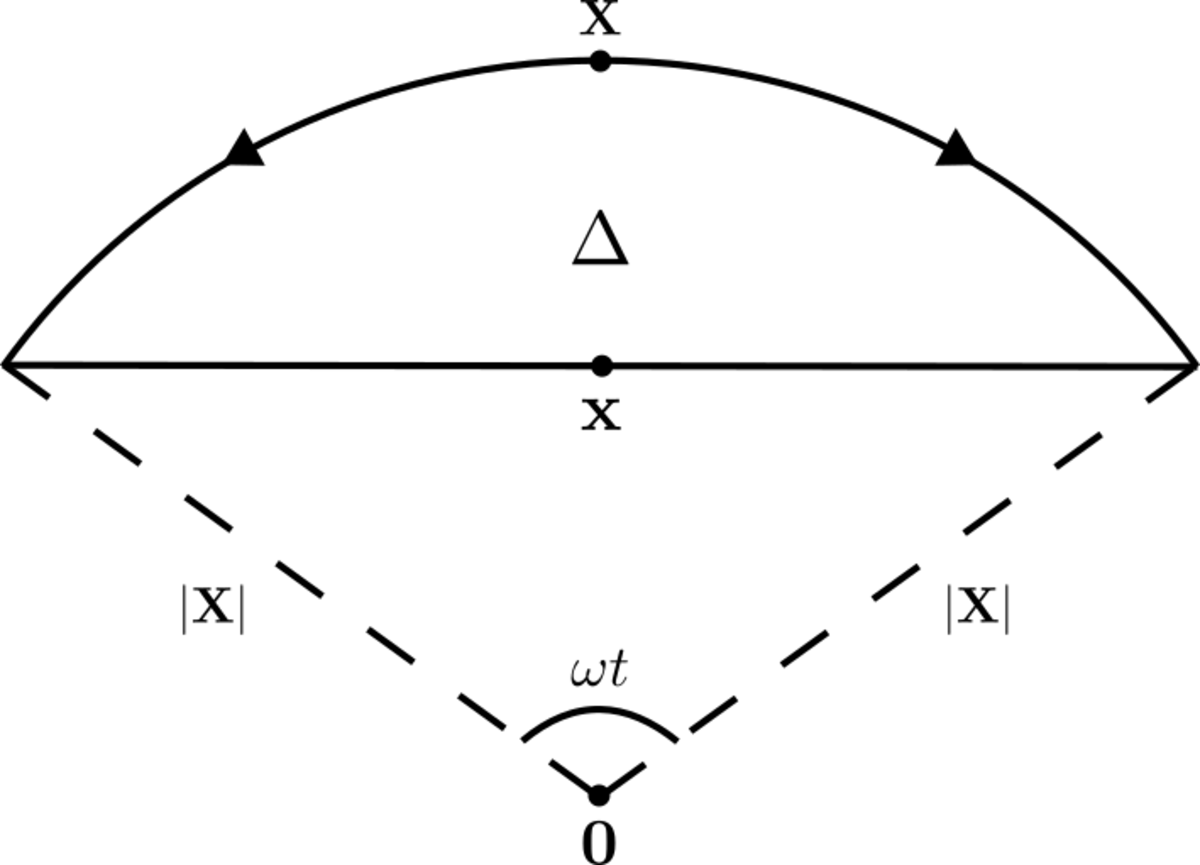
\includegraphics[width=0.6\textwidth]{Imagens/area_birkhoff.png}
    \centering
    \caption{$\Delta$ para hamiltonianas na forma \eqref{forma normal}.}
    \label{area birkhoff}
\end{figure}

Notamos que, nesse caso, o centro $\mathbf{x}$ fica determinado por
\begin{equation}
\label{centro real forma normal}
    \mathbf{x}\left( \mathbf{X},t \right) = \cos \left( \omega t \right) \mathbf{X},
\end{equation}
expressão esta que, se invertida e substituída em \eqref{ação real forma normal}, fornece $S(\mathbf{x},t)$. Para referência futura, observamos ainda que esta expressão permite o cálculo do determinante jacobiano da transformação $\mathbf{X} \mapsto \mathbf{x}$, o que nos dá
\begin{equation}
\label{det jac real forma normal}
    \det \frac{\partial \mathbf{x}}{\partial \mathbf{X}}(\mathbf{X},t) = \cos^2 \left( \omega t \right)\left[1 - 2 J \omega'  t \tan \left( \omega t \right) \right] .
\end{equation}

\section{Cáusticas e outras funções geratrizes}
\label{Cáusticas e outras funções geratrizes}

Da mesma forma que ocorre para as funções geratrizes usualmente estudadas, que tomam como argumento alguma combinação das coordenadas antigas $(p,q)$ e das coordenadas transformadas $(P,Q)$, existem certas classes de transformações canônicas que não são bem descritas pelas funções geratrizes de centros introduzidas na seção \ref{funções geratrizes}. De fato, a equação \eqref{jacobiano transformação canônica de centro} não é definida quando $\frac{1}{2}\mathbf{J} \partial^2 S/ \partial \mathbf{x}^2$ possui um autovalor $-1$. Alternativamente, invertendo esta relação, obtemos
\begin{equation}
    \frac{\mathbf{J}}{2} \frac{\partial^2 S}{\partial \mathbf{x}^2} = \left(\mathbf{I} - \frac{\partial \mathbf{x}_+}{\partial \mathbf{x}_-} \right) \left(\mathbf{I} + \frac{\partial \mathbf{x}_+}{\partial \mathbf{x}_-} \right)^{-1},
\end{equation}
que não é definida quando $\partial \mathbf{x}_+/\partial \mathbf{x}_-$ possui autovalor $-1$. Esses pontos problemáticos, que podem ser caracterizados pela equação
\begin{equation}
    \det \left(\mathbf{I} + \frac{\partial \mathbf{x}_+}{\partial \mathbf{x}_-} \right) = 0,
\end{equation}
são denominados de cáusticas.

Em particular, vemos que as funções geratrizes de centro não são capazes de descrever reflexões $R_{\mathbf{x}}$. Uma forma de entender essa falha é observar que, nesse caso, todos os pontos do espaço de fase compartilham o mesmo centro $\mathbf{x}$, de forma que não é possível determinar a corda em função do centro.

Para contornar esse problema, podemos definir uma nova classe de funções geratrizes complementares $\tilde{S}$ — as chamadas funções geratrizes de cordas — que, desta vez, determinam a transformação canônica ao fornecer o centro $\mathbf{x}$ como função da corda $\boldsymbol{\xi}$ através da expressão
\begin{equation}
    \mathbf{x} \left( \boldsymbol{\xi} \right) = \mathbf{J} \frac{\partial \tilde{S}}{\partial \boldsymbol{\xi}}.
\end{equation}
Nesse caso, temos
\begin{equation}
    \frac{\partial \mathbf{x}_{\pm}}{ \partial \boldsymbol{\xi}} =  \mathbf{J}\frac{\partial^2 \tilde{S}}{\partial \boldsymbol{\xi}^2} \pm \frac{\mathbf{I}}{2},
\end{equation}
o que nos permite obter
\begin{equation}
\label{jacobiano transformação canônica de corda}
    \frac{\partial \mathbf{x}_+}{ \partial \mathbf{x}_-} = \frac{\partial \mathbf{x}_+}{ \partial \boldsymbol{\xi}} \frac{\partial \boldsymbol{\xi}}{ \partial \mathbf{x}_-} = -\left(\mathbf{I} + 2 \mathbf{J} \frac{\partial^2 \tilde{S}}{\partial \boldsymbol{\xi}^2}\right) \left(\mathbf{I} - 2 \mathbf{J} \frac{\partial^2 \tilde{S}}{\partial \boldsymbol{\xi}^2}\right)^{-1},
\end{equation}
e, então,
\begin{equation}
    2 \mathbf{J} \frac{\partial^2 \tilde{S}}{\partial \boldsymbol{\xi}^2} = -\left(\mathbf{I} + \frac{\partial \mathbf{x}_+}{\partial \mathbf{x}_-} \right) \left(\mathbf{I} - \frac{\partial \mathbf{x}_+}{\partial \mathbf{x}_-} \right)^{-1}.
\end{equation}

Vemos que essa nova classe de funções geratrizes são bem comportadas na região em que as funções geratrizes de centro falham, mas, em compensação, quando $\partial \mathbf{x}_+/\partial \mathbf{x}_-$ tem autovalor $1$, como no caso da identidade, não estão bem definidas. Podemos ver, mais geralmente, que as funções geratrizes de corda não são capazes de descrever translações, pois desta vez, todos os pontos compartilham a mesma corda.

Observamos, por fim, que as expressões \eqref{jacobiano transformação canônica de centro} e \eqref{jacobiano transformação canônica de corda} que aqui reescrevemos de maneira genérica como
\begin{subequations}
    \begin{equation}
    \label{cayley 1}
        \mathbf{M} = \left( \mathbf{I}- \mathbf{JB} \right)\left( \mathbf{I}+ \mathbf{JB} \right)^{-1}
    \end{equation}
    \begin{equation}
        \mathbf{M} = -\left( \mathbf{I} + \mathbf{JB} \right)\left( \mathbf{I} - \mathbf{JB} \right)^{-1}
    \end{equation}
\end{subequations}
fornecem um mapa injetivo entre matrizes simétricas $\mathbf{B}$ — no nosso caso, representadas pelas hessianas das funções geratrizes — e matrizes simpléticas $\mathbf{M}$. Essa é a chamada parametrização de Cayley \cite{arnol2013dynamical} para matrizes simpléticas.

\chapter{A representação de Weyl-Wigner}
\label{A representação de Weyl-Wigner}

Neste capítulo, desenvolvemos a representação de Weyl-Wigner, que é base sobre a qual formularemos todos os resultados dessa dissertação. Se trata de uma representação da mecânica quântica feita no espaço de fase, tornando-a uma linguagem natural para se discutir limites clássicos e semiclássicos.

Começaremos definindo operadores de translação e reflexão, que são análogos às transformações clássicas definidas na seção \ref{Sistemas hamiltonianos e transformações canônicas}. Depois expandimos um operador qualquer como uma combinação linear de um desses operadores, sendo os coeficientes dessa expansão funções definidas sobre o espaço de fase, a partir das quais podemos calcular qualquer quantidade de interesse. Por fim, utilizamos essa representação para obter uma expressão para o propagador em termos de uma integral de caminhos, e discutimos o seu limite semiclássico.

\section{Operadores de Translação e Reflexão}

A representação de Weyl-Wigner é baseada em operadores de translação e reflexão, que são a versão quântica das transformações já introduzidas na seção \ref{Sistemas hamiltonianos e transformações canônicas}. Começaremos definindo os operadores de translação, que, em termos dos operadores de posição $\hat{q}$ e momento $\hat{p}$, têm uma fórmula relativamente simples, e, a partir deles, definiremos os operadores de reflexão. 

Para isso, consideramos primeiramente um espaço de Hilbert genérico sobre o qual está definido um operador hermitiano $\hat{A}$ cujos autoestados $\ket{A}$ são tais que $\hat{A} \ket{A} = A \ket{A}$, onde $A \in \mathbb{R}$. Sendo $\hat{B}$ um operador tal que $\comm{\hat{A}}{\hat{B}} = i \hat{I}$, é possível mostrar que, para qualquer função analítica $F$, vale $\comm{\hat{A}}{F\left(\hat{B}\right)} = i F' \left( \hat{B} \right)$ \cite{cohen2019quantum}. Desta forma definindo o operador
\begin{equation}
    \hat{T}_a = \exp \left( -i a \hat{B} \right),
\end{equation}
vemos que $\comm{\hat{A} }{\hat{T}_a} = a\hat{T}_a$, e, então,
\begin{equation}
    \hat{A} \hat{T}_a \ket{A} = \hat{T}_a \left(\hat{A} + a \hat{I}\right) \ket{A} = \left(A + a\right)\hat{T}_a \ket{A} \Rightarrow \hat{T}_a \ket{A}  = \ket{A+a},
\end{equation}
isto é, $\hat{T}_a$ é um operador de translação. Fazendo uso da relação de comutação canônica $\comm{\hat{q}}{\hat{p}} = i \hbar \hat{I}$ concluímos que $\hat{T}_p = \exp \left( i p \hat{q}/\hbar \right)$ é o operador de translação sobre os momentos enquanto que $\hat{T}_q = \exp \left( -i q \hat{p}/\hbar \right)$ é o operador de translação sobre as posições. Estamos interessados no operador que realiza a translação no espaço de fase, isto é, tanto nas posições como nos momentos, o chamado operador de Heisenberg, que definimos como
\begin{equation}
    \label{def_heisenberg}
    \hat{T}_{\boldsymbol{\xi}} = \exp \left( \frac{i}{\hbar} \boldsymbol{\xi} \wedge \hat{\mathbf{x}} \right) = \exp \left[ \frac{i}{\hbar} \left(\xi_p \cdot \hat{q}-\xi_q \cdot \hat{p}\right) \right], \ \ \ \boldsymbol{\xi} = (\xi_p,\xi_q) \in \mathbb{R}^2; \ \ \ \hat{\mathbf{x}} = \left( \hat{p},\hat{q} \right).
\end{equation}
A generalização do operador de Heisenberg para um sistema com $d$ graus de liberdade, que utilizaremos a partir daqui, é imediata, bastando substituir, $\hat{p}$ por $\hat{\mathbf{p}} = \left( \hat{p}_1,\ldots,\hat{p}_d \right)$, $\xi_p$ por $\boldsymbol{\xi}_p \in \mathbb{R}^d$, e analogamente para $\hat{q}$ e $\xi_q$.

No caso em que $\hat{A}$ e $\hat{B}$ comutam com o seu comutador, como acontece para $\hat{p}_j$ e $\hat{q}_j$, a fórmula de Baker–Campbell–Hausdorff (BCH) nos diz que
\begin{equation}
    \label{BCH}
    \exp \left(\hat{A}\right)\exp \left(\hat{B}\right) = \exp \left(\hat{A} + \hat{B} + \frac{1}{2}\comm{\hat{A}}{\hat{B}}\right)
\end{equation}
o que nos permite separar $\hat{T}_{\boldsymbol{\xi}}$ como
\begin{equation}
    \hat{T}_{\boldsymbol{\xi}} = \exp\left(- \frac{i}{2\hbar}\boldsymbol{\xi}_p \cdot \boldsymbol{\xi}_q\right) \hat{T}_{\boldsymbol{\xi}_p} \hat{T}_{\boldsymbol{\xi}_q} = \exp\left(\frac{i}{2\hbar}\boldsymbol{\xi}_p \cdot\boldsymbol{\xi}_q\right)\hat{T}_{\boldsymbol{\xi}_q} \hat{T}_{\boldsymbol{\xi}_p}
\end{equation}

Notamos ainda que o traço de $\hat{T}_{\boldsymbol{\xi}}$ é
\begin{equation}
\label{traço t}
    \begin{aligned}
        \Tr \hat{T}_{\boldsymbol{\xi}} &= \int d\mathbf{q} \ev{\hat{T}_{\boldsymbol{\xi}}}{\mathbf{q}} \\ &=  \int d\mathbf{q} \exp\left(- \frac{i}{2\hbar}\boldsymbol{\xi}_p \cdot\boldsymbol{\xi}_q\right) \ev{\hat{T}_{\boldsymbol{\xi}_p} \hat{T}_{\boldsymbol{\xi}_q} }{\mathbf{q}}
        \\ &=  \exp\left(\frac{i}{2\hbar} \boldsymbol{\xi}_p \cdot\boldsymbol{\xi}_q \right)\int d\mathbf{q} \exp\left(\frac{i}{\hbar}\boldsymbol{\xi}_p\cdot \mathbf{q} \right) \innerproduct{\mathbf{q}}{\mathbf{q}+\boldsymbol{\xi}_q} \\
        &= \left(2\pi \hbar\right)^d \delta(\boldsymbol{\xi}),
    \end{aligned}
\end{equation}
e que $\hat{T}_{\boldsymbol{\xi}}$ não é hermitiano, já que, de \eqref{def_heisenberg}, decorre que
\begin{equation}
\label{adjunta T}
    \hat{T}_{\boldsymbol{\xi}}^\dagger = \hat{T}_{\boldsymbol{-\xi}}.
\end{equation}

Definiremos os operadores de reflexão por
\begin{equation}
    \label{def_reflexão}
    \hat{R}_\mathbf{x} = \frac{1}{\left(4\pi \hbar \right)^d} \int d \boldsymbol{\xi} \exp \left( \frac{i}{\hbar} \mathbf{x} \wedge \boldsymbol{\xi} \right) \hat{T}_{\boldsymbol{\xi}},
\end{equation}
e a justificativa para essa definição ficará mais clara a seguir, mas antes, notaremos alguma de suas propriedades. Primeiramente, de \eqref{adjunta T} e \eqref{def_reflexão}, deduzimos que $\hat{R}_\mathbf{x}$ é hermitiano. Além disso, combinando \eqref{traço t} e \eqref{def_reflexão}, concluímos que o traço de $\hat{R}_\mathbf{x}$ é dado por
\begin{equation}
    \Tr \hat{R}_\mathbf{x} = \frac{1}{2^d}.
\end{equation}
Por fim, observamos que podemos inverter \eqref{def_reflexão}, obtendo
\begin{equation}
    \label{inversão}
    \begin{aligned}
        \hat{T}_{\boldsymbol{\xi}} &= \int d \boldsymbol{\xi}' \ \delta\left(\boldsymbol{\xi}' - \boldsymbol{\xi}\right) \hat{T}_{\boldsymbol{\xi}'} \\
        &= \frac{1}{\left(2\pi \hbar\right)^{2d}} \int d\mathbf{x}d \boldsymbol{\xi}' \ \exp \left[-\frac{i}{\hbar} \mathbf{x} \wedge \left(\boldsymbol{\xi} - \boldsymbol{\xi} '\right)\right] \hat{T}_{\boldsymbol{\xi}'} \\
        &= \frac{1}{\left(\pi \hbar\right)^d} \int d\mathbf{x} \ \exp \left(-\frac{i}{\hbar} \mathbf{x} \wedge \boldsymbol{\xi} \right) \hat{R}_\mathbf{x}
    \end{aligned}.
\end{equation}

A justificativa para chamar $\hat{R}_\mathbf{x}$ de um operador de reflexão vem do fato de que esses operadores, em conjunto com os $\hat{T}_{\boldsymbol{\xi}}$, reproduzem relações análogas às relações clássicas \eqref{reflexões e translações clássicas}:
\begin{lema}
    \label{composição operadores translação reflexão}
    Os operadores de reflexão e translação satisfazem as relações
    \begin{subequations}
    \begin{equation}
    \label{trans trans}
        \hat{T}_{\boldsymbol{\xi}_2} \hat{T}_{\boldsymbol{\xi}_1} = \exp\left(-\frac{i}{2\hbar}\boldsymbol{\xi}_1 \wedge \boldsymbol{\xi}_2\right) \hat{T}_{\boldsymbol{\xi}_1+\boldsymbol{\xi}_2} 
    \end{equation}
    \begin{equation}
    \label{ref trans}
         \hat{R}_\mathbf{x} \hat{T}_{\boldsymbol{\xi}}= \exp\left(-\frac{i}{\hbar}\mathbf{x} \wedge \boldsymbol{\xi}\right) \hat{R}_{\mathbf{x}-\boldsymbol{\xi}/2}
    \end{equation}
    \begin{equation}
    \label{trans ref}
       \hat{T}_{\boldsymbol{\xi}} \hat{R}_\mathbf{x} = \exp\left(-\frac{i}{\hbar}\mathbf{x} \wedge \boldsymbol{\xi}\right) \hat{R}_{\mathbf{x}+\boldsymbol{\xi}/2}
    \end{equation}
    \begin{equation}
    \label{ref ref}
        \hat{R}_{\mathbf{x}_2} \hat{R}_{\mathbf{x}_1} = \exp\left(\frac{2i}{\hbar}\mathbf{x}_1 \wedge \mathbf{x}_2\right) \hat{T}_{2(\mathbf{x}_2-\mathbf{x}_1)}
    \end{equation}
    \end{subequations}
\end{lema}

\begin{proof}

    A expressão \eqref{trans trans} decorre imediatamente de \eqref{def_heisenberg} e \eqref{BCH}.

    Para demonstrar \eqref{ref trans} utilizamos \eqref{def_reflexão} e \eqref{trans trans}:
    \begin{equation}
        \begin{aligned}
            \hat{R}_\mathbf{x} \hat{T}_{\boldsymbol{\xi}} &= \frac{1}{\left(4\pi \hbar\right)^n} \int d \boldsymbol{\xi}' \ \exp \left(\frac{i}{\hbar}\mathbf{x} \wedge \boldsymbol{\xi} '\right) \hat{T}_{\boldsymbol{\xi}'} \hat{T}_{\boldsymbol{\xi}} \\
            &= \frac{1}{\left(4\pi \hbar\right)^n} \int d \boldsymbol{\xi}' \ \exp \left[\frac{i}{\hbar}\left(\mathbf{x} - \frac{1}{2}\boldsymbol{\xi}\right) \wedge \boldsymbol{\xi} '\right] \hat{T}_{\boldsymbol{\xi}+\boldsymbol{\xi}'} \\
            &= \frac{1}{\left(4\pi \hbar\right)^n} \int d \boldsymbol{\eta} \ \exp \left[\frac{i}{\hbar}\left(\mathbf{x} - \frac{1}{2}\boldsymbol{\xi}\right) \wedge \left(\boldsymbol{\eta} - \boldsymbol{\xi} \right)\right] \hat{T}_{\boldsymbol{\eta}} \\ &= \exp \left( -\frac{i}{\hbar} \mathbf{x} \wedge \boldsymbol{\xi}\right) \hat{R}_{\mathbf{x}-\boldsymbol{\xi}/2},
        \end{aligned}
    \end{equation}
    sendo demonstração de \eqref{trans ref} análoga.
    Já \eqref{ref ref} decorre de \eqref{def_reflexão}, \eqref{inversão} e de \eqref{trans ref}:
    \begin{equation}
        \begin{aligned}
            \hat{R}_{\mathbf{x}_2} \hat{R}_{\mathbf{x}_1} &= \frac{1}{\left(4\pi \hbar\right)^n} \int d \boldsymbol{\xi} \exp\left(\frac{i}{\hbar}\mathbf{x}_2 \wedge \boldsymbol{\xi}\right) \hat{T}_{\boldsymbol{\xi}} \hat{R}_{\mathbf{x}_1} \\
            &= \frac{1}{\left(4\pi \hbar\right)^n} \int d \boldsymbol{\xi} \exp\left[\frac{i}{\hbar}\left(\mathbf{x}_2-\mathbf{x}_1\right) \wedge \boldsymbol{\xi}\right] \hat{R}_{\mathbf{x}_1+\boldsymbol{\xi}/2} \\
            &= \frac{1}{\left(\pi \hbar\right)^n} \int d \boldsymbol{\xi} \exp\left[\frac{2i}{\hbar}\left(\mathbf{x}_2-\mathbf{x}_1\right) \wedge \left(\boldsymbol{\eta}-\mathbf{x}_1\right)\right] \hat{R}_{\boldsymbol{\eta}} \\ &= \exp \left( \frac{2i}{\hbar} \mathbf{x}_1 \wedge \mathbf{x}_2 \right) \hat{T}_{2(\mathbf{x}_2-\mathbf{x}_1)}
        \end{aligned}
    \end{equation}
\end{proof}

Supondo que os operadores de reflexão formam uma base para o espaço dos operadores, podemos decompor um operador arbitrário $\hat{A}$ como
\begin{equation}
\label{expansao A}
    \hat{A} = \frac{1}{\left(\pi \hbar\right)^d} \int d\mathbf{x} A(\mathbf{x}) \hat{R}_\mathbf{x}.
\end{equation}
Os coeficientes $A(\mathbf{x})$ desta expansão, conhecidos como o símbolo de Wigner do operador $\hat{A}$, podem ser obtidos como
\begin{equation}
    \begin{aligned}
        2^d \Tr \left( \hat{A} \hat{R}_\mathbf{x} \right) &= \left( \frac{2}{\pi \hbar} \right)^d \int d\mathbf{x}' A\left(\mathbf{x}'\right) \Tr \left(\hat{R}_{\mathbf{x}'}\hat{R}_\mathbf{x}\right) \\
        &=  \left( \frac{2}{\pi \hbar} \right)^d \int d\mathbf{x}' A\left(\mathbf{x}'\right) \exp \left( \frac{2i}{\hbar} \mathbf{x} \wedge \mathbf{x}' \right) \Tr \left(\hat{T}_{2(\mathbf{x}'-\mathbf{x})}\right) \\
        &=  2^{2d} \int d\mathbf{x}' A\left(\mathbf{x}'\right) \exp \left( \frac{2i}{\hbar} \mathbf{x} \wedge \mathbf{x}' \right)\delta\left[2\left(\mathbf{x}'-\mathbf{x}\right)\right] \\
        &= A(\mathbf{x}),
    \end{aligned}
\end{equation}
e são funções definidas no espaço de fase. Combinando a equação \eqref{expansao A} com o fato de que $\hat{R}_\mathbf{x}^\dagger = \hat{R}_\mathbf{x}$, concluímos que, quando $\hat{A}$ é hermitiano, então $A(\mathbf{x})$ é real.

Tendo em vista que
\begin{equation}
    \hat{T}_{\boldsymbol{\xi}} \ket{\mathbf{q}_{-}} = \exp \left[\frac{i}{\hbar} \boldsymbol{\xi}_p \cdot \left( \mathbf{q}_- + \frac{\boldsymbol{\xi}_q}{2} \right) \right] \ket{\mathbf{q}_- + \boldsymbol{\xi}_q},
\end{equation}
obtém-se
\begin{equation}
    \begin{aligned}
        \hat{R}_\mathbf{x} \ket{\mathbf{q}_-} &= \frac{1}{\left(4\pi \hbar\right)^d} \int d \boldsymbol{\xi} \exp \left\{\frac{i}{\hbar} \left[\boldsymbol{\xi}_p \cdot\left( \mathbf{q}_- + \frac{\boldsymbol{\xi}_q}{2} -\mathbf{q}\right) + \mathbf{p} \cdot \boldsymbol{\xi}_q \right] \right\} \ket{\mathbf{q}_- + \boldsymbol{\xi}_q} \\
        &= \frac{1}{2^d} \int d \boldsymbol{\xi}_q \delta\left( \mathbf{q}_- + \frac{\boldsymbol{\xi}_q}{2} -\mathbf{q}\right) \exp \left( \frac{i}{\hbar} \mathbf{p} \cdot \boldsymbol{\xi}_q \right) \ket{\mathbf{q}_-+\boldsymbol{\xi}_q} \\
        &= \exp \left[ \frac{2i}{\hbar} \mathbf{p} \cdot \left(\mathbf{q}-\mathbf{q}_-\right) \right] \ket{2\mathbf{q}-\mathbf{q}_-},
    \end{aligned}
\end{equation}
e, então,
\begin{equation}
    \begin{aligned}
        \mel{\mathbf{q}_+}{\hat{R}_\mathbf{x}}{\mathbf{q}_-} &= \exp \left[ \frac{2i}{\hbar} \mathbf{p} \cdot \left(\mathbf{q}-\mathbf{q}_-\right) \right] \delta \left(2\mathbf{q}-\mathbf{q}_+-\mathbf{q}_-\right) \\
        &= \frac{1}{2^d} \exp \left[ \frac{i}{\hbar} \mathbf{p} \cdot \left(\mathbf{q}_+-\mathbf{q}_-\right) \right] \delta \left(\mathbf{q}-\frac{\mathbf{q}_++\mathbf{q}_-}{2}\right).
    \end{aligned}
\end{equation}
Este elemento de matriz nos permite calcular a símbolo de Wigner de um operador $\hat{A}$ em termos de sua representação de posição:
\begin{equation}
    \begin{aligned}
        A(\mathbf{x}) &= 2^d \Tr \left(\hat{A}\hat{R}_\mathbf{x}\right) \\ &= 2^d \int d\mathbf{q}_- d\mathbf{q}_+ \ \mel{\mathbf{q}_+}{\hat{A}}{\mathbf{q}_-} \mel{\mathbf{q}_-}{\hat{R}_\mathbf{x}}{\mathbf{q}_+} \\
        & =  \int d\mathbf{q}_- d\mathbf{q}_+ \ \mel{\mathbf{q}_+}{\hat{A}}{\mathbf{q}_-} \exp \left[ -\frac{i}{\hbar} \mathbf{p} \cdot \left(\mathbf{q}_+-\mathbf{q}_-\right) \right] \delta \left(\mathbf{q}-\frac{\mathbf{q}_++\mathbf{q}_-}{2}\right).
    \end{aligned}
\end{equation}
Realizando a mudança de coordenadas
\begin{equation}
    \begin{cases}
        \boldsymbol{\xi}_q = \mathbf{q}_+-\mathbf{q}_- \\
        \tilde{\mathbf{q}} = \dfrac{\mathbf{q}_++\mathbf{q}_-}{2}
    \end{cases},
\end{equation}
cujo determinante jacobiano é $1$, obtemos
\begin{equation}
    A(\mathbf{x}) = \int d \boldsymbol{\xi}_q \mel{\mathbf{q}+\frac{1}{2}\boldsymbol{\xi}_q}{\hat{A}}{\mathbf{q}-\frac{1}{2}\boldsymbol{\xi}_q}\exp \left( -\frac{i}{\hbar} \mathbf{p} \cdot \boldsymbol{\xi}_q \right),
\end{equation}
e um procedimento análogo nos permite obter
\begin{equation}
    A\left(\mathbf{x}\right) = \int d \boldsymbol{\xi}_p \mel{\mathbf{p}+\frac{1}{2}\boldsymbol{\xi}_p}{\hat{A}}{\mathbf{p}-\frac{1}{2}\boldsymbol{\xi}_p}\exp \left( \frac{i}{\hbar} \mathbf{q} \cdot \boldsymbol{\xi}_p \right).
\end{equation}
Um resultado importante que pode ser obtido dessas fórmulas é o fato de que o símbolo de Wigner de $f\left(\hat{\mathbf{q}}\right)$ é $f(\mathbf{q})$, enquanto que a símbolo de Wigner de $f\left(\hat{\mathbf{p}}\right)$ é $f(\mathbf{p})$, onde $f$ é uma função arbitrária.

A símbolo de Wigner do operador densidade $\hat{\rho}$ é de especial importância, e sua versão normalizada $W\left(\mathbf{x}\right) = \rho\left(\mathbf{x}\right)/(2\pi \hbar)^d$ é a chamada função de Wigner. Como
\begin{equation}
    \rho\left(\mathbf{x}\right) = 2^d \Tr \left(\hat{\rho} \hat{R}_\mathbf{x}\right) = 2^d \ev{\hat{R}_\mathbf{x}},
\end{equation}
vemos que $W\left(\mathbf{x}\right)$ é proporcional ao valor esperado $\ev{\hat{R}_\mathbf{x}}$ no estado $\hat{\rho}$. Além disso, no caso de um estado puro descrito por um vetor $\ket{\psi}$, temos
\begin{equation}
\label{função de wigner em termos de função de onda}
    W\left(\mathbf{x}\right) = \frac{1}{(2\pi \hbar)^d} \int d \boldsymbol{\xi}_q \psi\left(\mathbf{q}+\frac{1}{2}\boldsymbol{\xi}_q\right) \psi^*\left(\mathbf{q}-\frac{1}{2}\boldsymbol{\xi}_q\right) \exp \left( -\frac{i}{\hbar} \mathbf{p} \cdot \boldsymbol{\xi}_q \right),
\end{equation}
de forma que a função de Wigner também pode ser interpretada como a transformada de Fourier da correlação espacial da função de onda.

A nível de exemplo, observamos que a função de Wigner correspondente aos autoestados do oscilador harmônico, definido por uma hamiltoniana $\hat{H} = \omega \left( \hat{p}^2+\hat{q}^2 \right)/2$, são dadas por
\begin{equation}
\label{função de wigner do oscilador harmônico}
    W_n(\mathbf{x}) = \frac{(-1)^n}{\pi \hbar} e^{-\mathbf{x}^2/\hbar}L_n\left( \frac{2 \mathbf{x}^2}{\hbar} \right),
\end{equation}
onde $L_n$ é o $n$-ésimo polinômio de Laguerre \cite{GROENEWOLD1946405}. 

Existe também a possibilidade de representar um operador $\hat{A}$ como uma superposição de translações:
\begin{equation}
    \hat{A} = \frac{1}{\left(2 \pi \hbar\right)^d} \int d \boldsymbol{\xi} A(\boldsymbol{\xi}) \hat{T}_{\boldsymbol{\xi}}
\end{equation}
e o coeficiente $A(\boldsymbol{\xi})$, denominado símbolo de Weyl do operador $\hat{A}$, pode ser obtido explicitamente como
\begin{equation}
    \Tr \left(\hat{T}_{-\boldsymbol{\xi}}\hat{A}\right) = \frac{1}{\left(2 \pi \hbar\right)^d} \int d \boldsymbol{\xi}' A\left(\boldsymbol{\xi}'\right) \Tr \left(\hat{T}_{-\boldsymbol{\xi}}\hat{T}_{\boldsymbol{\xi}'}\right) = A\left(\boldsymbol{\xi}\right).
\end{equation}
Na verdade, existe uma conexão próxima entre $A(\mathbf{x})$ e $A\left(\boldsymbol{\xi}\right)$. Para ver isso, notamos que, de acordo com \eqref{def_reflexão} e \eqref{inversão}, temos
\begin{equation}
    R_{\mathbf{x}}\left(\boldsymbol{\xi}\right) = \frac{1}{2^d} \exp\left(\frac{i}{\hbar}\mathbf{x}\wedge\boldsymbol{\xi}\right);
\end{equation}
\begin{equation}
    T_{\boldsymbol{\xi}}\left(\mathbf{x}\right) =  \exp\left(-\frac{i}{\hbar}\mathbf{x}\wedge\boldsymbol{\xi}\right),
\end{equation}
e, então
\begin{equation}
    \label{wigner em termos de weyl}
    A \left(\mathbf{x}\right) = \frac{1}{\left(2 \pi \hbar\right)^d} \int d \boldsymbol{\xi} A(\boldsymbol{\xi}) \exp\left(-\frac{i}{\hbar}\mathbf{x}\wedge\boldsymbol{\xi}\right);
\end{equation}
\begin{equation}
    A\left(\boldsymbol{\xi}\right) = \frac{1}{\left(2\pi \hbar\right)^d} \int d\mathbf{x} A(\mathbf{x}) \exp\left(\frac{i}{\hbar}\mathbf{x}\wedge\boldsymbol{\xi}\right),
\end{equation}
isto é, os símbolos de Weyl-Wigner estão conectados por uma transformada de Fourier simplética, que difere da transformada de Fourier usual por um sinal na exponencial correspondente a metade das coordenadas.

\section{Representação de Weyl-Wigner da composição de operadores}
\label{Representação de Weyl-Wigner da composição de operadores}

Para começar a utilizar a representação de Weyl-Wigner para cálculos práticos, será fundamental discutir como se dá a composição de operadores. Começamos notando que, utilizando o lema \ref{composição operadores translação reflexão} $N$ vezes, obtemos
\begin{equation}
    \hat{T}_{\boldsymbol{\xi}_N} \cdots \hat{T}_{\boldsymbol{\xi}_1} = \exp\left[-\frac{i}{\hbar}D_{N+1}\left(\boldsymbol{\xi}_1,\ldots,\boldsymbol{\xi}_N\right)\right] \hat{T}_{\boldsymbol{\xi}}, \ \ \  \boldsymbol{\xi} = \sum_{j=1}^N \boldsymbol{\xi}_j
\end{equation}
sendo
\begin{equation}
    \label{área em termos das cordas}
    \begin{aligned}
        D_{N+1}\left(\boldsymbol{\xi}_1,\ldots,\boldsymbol{\xi}_N\right) &= \frac{1}{2}\left[\boldsymbol{\xi}_1 \wedge \boldsymbol{\xi}_2 + \left(\boldsymbol{\xi}_1+\boldsymbol{\xi}_2\right)\wedge\boldsymbol{\xi}_3 + \cdots \left(\boldsymbol{\xi}_1 + \cdots \boldsymbol{\xi}_{N-1}\right)\wedge\boldsymbol{\xi}_N\right] \\
        &= \frac{1}{2} \sum_{j < k} \boldsymbol{\xi}_j \wedge \boldsymbol{\xi}_k,
    \end{aligned}
\end{equation}
que é precisamente a área do polígono de lados $\boldsymbol{\xi},\boldsymbol{\xi}_1,\ldots\boldsymbol{\xi}_N$, o que pode ser visto ao decompô-lo em triângulos, como na figura \ref{area em termos da corda}.

\begin{figure}[H]
    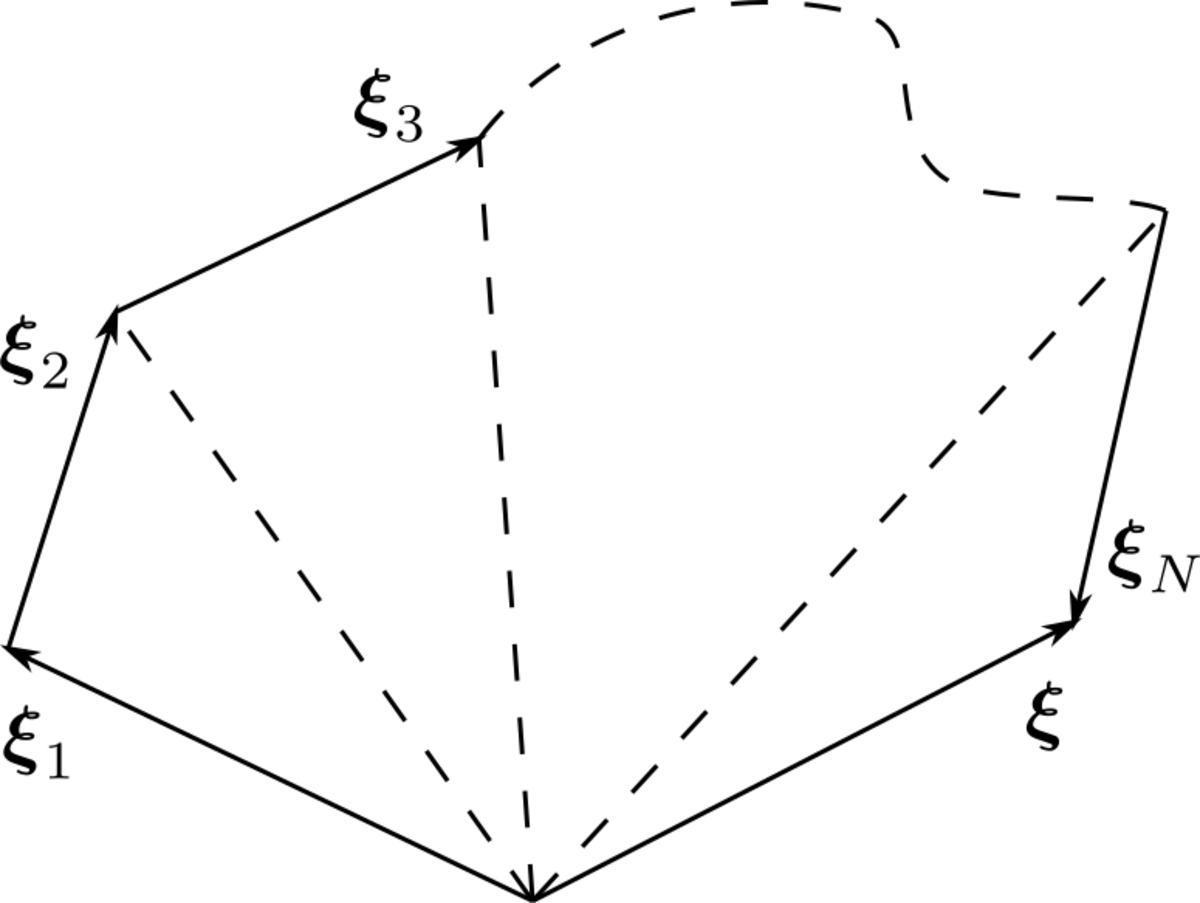
\includegraphics[width=.5\textwidth]{Imagens/area_em_termos_da_corda.png}
    \centering
    \caption{Decomposição de um polígono em triângulos}
    \label{area em termos da corda}
\end{figure}

Com isso, temos
\begin{equation}
    \begin{aligned}
        A_N \cdots A_1 \left(\boldsymbol{\xi}\right) &= \frac{1}{\left(2 \pi \hbar\right)^{Nd}}\int \prod_{j=1}^N d \boldsymbol{\xi}_j A_j \left(\boldsymbol{\xi}_j\right) \Tr \left(\hat{T}_{-\boldsymbol{\xi}} \hat{T}_{\boldsymbol{\xi}_N}\cdots \hat{T}_{\boldsymbol{\xi}_1}\right) \\
        & = \frac{1}{\left(2 \pi \hbar\right)^{(N-1)d}}\int \prod_{j=1}^N d \boldsymbol{\xi}_j A_j \left(\boldsymbol{\xi}_j\right) \exp\left[-\frac{i}{\hbar}D_{N+1}\left(\boldsymbol{\xi}_1,\ldots,\boldsymbol{\xi}_N\right)\right] \\ & \qquad \qquad \qquad  \times\delta\left(\boldsymbol{\xi}_1+\cdots+\boldsymbol{\xi}_N-\boldsymbol{\xi}\right)
    \end{aligned}
\end{equation}

Tomando a transformada de Fourier simplética, como em \eqref{wigner em termos de weyl}, e utilizando a $\delta$ para eliminar a integral em $\boldsymbol{\xi}$, chegamos a
\begin{equation}
    \begin{aligned}
        A_N \cdots A_1 \left(\mathbf{x}\right) = \frac{1}{\left(2 \pi \hbar\right)^{Nd}}\int \prod_{j=1}^N d \boldsymbol{\xi}_j & A_j \left(\boldsymbol{\xi}_j\right) \exp\left(-\frac{i}{\hbar} \mathbf{x}\wedge\boldsymbol{\xi}_j\right) \\ &\times \exp\left[-\frac{i}{\hbar}D_{N+1}\left(\boldsymbol{\xi}_1,\ldots,\boldsymbol{\xi}_N\right)\right] 
    \end{aligned}
\end{equation}

Para avaliar esta expressão, é conveniente introduzir a função auxiliar
\begin{equation}
    \begin{aligned}
        f(\mathbf{x}_1,\ldots,\mathbf{x}_N) = \frac{1}{\left(2 \pi \hbar\right)^{Nd}}\int \prod_{j=1}^N d \boldsymbol{\xi}_j & A_j \left(\boldsymbol{\xi}_j\right) \exp\left(-\frac{i}{\hbar} \mathbf{x}_j\wedge\boldsymbol{\xi}_j\right) \\ &\times \exp\left[-\frac{i}{\hbar}D_{N+1}\left(\boldsymbol{\xi}_1,\ldots,\boldsymbol{\xi}_N\right)\right],
    \end{aligned}
\end{equation}
que satisfaz $A_N \cdots A_1 \left(\mathbf{x}\right) = f(\mathbf{x},\ldots,\mathbf{x})$. Agora, observando que
\begin{equation}
    \begin{aligned}
        \left(\frac{\partial}{\partial \mathbf{x}_j} \wedge \frac{\partial}{\partial \mathbf{x}_k}\right) &\exp\left[-\frac{i}{\hbar} \left(\mathbf{x}_j\wedge\boldsymbol{\xi}_j + \mathbf{x}_k\wedge\boldsymbol{\xi}_k\right)\right] \\ =  -\frac{1}{\hbar^2} \boldsymbol{\xi}_j \wedge \boldsymbol{\xi}_k &\exp\left[-\frac{i}{\hbar} \left(\mathbf{x}_j\wedge\boldsymbol{\xi}_j + \mathbf{x}_k\wedge\boldsymbol{\xi}_k\right)\right]
    \end{aligned}
\end{equation}
e utilizando \eqref{área em termos das cordas}, vemos que
\begin{equation}
    \begin{aligned}
        i \hbar D_{N+1}\left(\frac{\partial}{\partial \mathbf{x}_1},\ldots,\frac{\partial}{\partial \mathbf{x}_N}\right) &\prod_{j=1}^N  \exp\left(-\frac{i}{\hbar} \mathbf{x}_j\wedge\boldsymbol{\xi}_j\right) \\ 
        =-\frac{i}{\hbar}D_{N+1}\left(\boldsymbol{\xi}_1,\ldots,\boldsymbol{\xi}_N\right) &\prod_{j=1}^N  \exp\left(-\frac{i}{\hbar} \mathbf{x}_j\wedge\boldsymbol{\xi}_j\right),
    \end{aligned}
\end{equation}
o que nos permite escrever
\begin{equation}
    \begin{aligned}
        \exp \left[i \hbar D_{N+1}\left(\frac{\partial}{\partial \mathbf{x}_1},\ldots,\frac{\partial}{\partial \mathbf{x}_N}\right)\right] &\prod_{j=1}^N  \exp\left(-\frac{i}{\hbar} \mathbf{x}_j\wedge\boldsymbol{\xi}_j\right) \\ 
        =\exp\left[-\frac{i}{\hbar}D_{N+1}\left(\boldsymbol{\xi}_1,\ldots,\boldsymbol{\xi}_N\right)\right] &\prod_{j=1}^N  \exp\left(-\frac{i}{\hbar} \mathbf{x}_j\wedge\boldsymbol{\xi}_j\right),
    \end{aligned}
\end{equation}
e, então
\begin{equation}
    \begin{aligned}
        f(\mathbf{x}_1,\ldots,\mathbf{x}_N) &= \frac{1}{\left(2 \pi \hbar\right)^{Nd}}\exp \left[i \hbar D_{N+1}\left(\frac{\partial}{\partial \mathbf{x}_1},\ldots,\frac{\partial}{\partial \mathbf{x}_N}\right)\right] \\ & \qquad \qquad \qquad \int \prod_{j=1}^N d \boldsymbol{\xi}_j A_j \left(\boldsymbol{\xi}_j\right) \exp\left(-\frac{i}{\hbar} \mathbf{x}_j\wedge\boldsymbol{\xi}_j\right) \\
        &=\exp \left[i \hbar D_{N+1}\left(\frac{\partial}{\partial \mathbf{x}_1},\ldots,\frac{\partial}{\partial \mathbf{x}_N}\right)\right] A_N\left(\mathbf{x}_N\right) \cdots A_1\left(\mathbf{x}_1\right)
    \end{aligned}
\end{equation}
o que nos permite obter $A_N \cdots A_1 \left(\mathbf{x}\right)$ em termos de $A_1\left(\mathbf{x}\right),\ldots,A_N\left(\mathbf{x}\right)$. Vemos que
\begin{equation}
    A_m \cdots A_1 \left(\mathbf{x}\right) = A_m \left( \mathbf{x} \right) \cdots A_1 \left( \mathbf{x} \right) + \order{\hbar}
\end{equation}
e, se $A_m \cdots A_1$ é hermitiano, então a correção é da ordem de $\hbar^2$.
No caso particularmente importante de dois operadores, obtemos
\begin{equation}
\label{groenewold}
    \begin{aligned}
        A_2 \cdot A_1 \left(\mathbf{x}\right) &= \exp\left(\frac{i \hbar}{2} \frac{\partial}{\partial \mathbf{x}_1} \wedge \frac{\partial}{\partial \mathbf{x}_2}\right) A_2\left(\mathbf{x}_1\right)  A_1\left(\mathbf{x}_2\right) \eval_{\mathbf{x}_1 = \mathbf{x},\ \mathbf{x}_2=\mathbf{x}}    \\ & =A_2\left(\mathbf{x}+\frac{i \hbar}{2}\mathbf{J}\frac{\partial}{\partial \mathbf{x}}\right)  A_1\left(\mathbf{x}\right) \\ & =A_1\left(\mathbf{x}-\frac{i \hbar}{2}\mathbf{J}\frac{\partial}{\partial \mathbf{x}}\right)  A_2\left(\mathbf{x}\right),
    \end{aligned}
\end{equation}
que é a chamada regra de Groenewold.

Em particular, podemos utilizar esta fórmula para mostrar que
\begin{equation}
\label{expansão segunda ordem}
    \hat{A}^2 \left( \mathbf{x}\right) = \left[A\left( \mathbf{x}\right)\right]^2 + \frac{\hbar^2}{8} \Tr \left[\left( \mathbf{J} \boldsymbol{\mathcal{H}_{\mathbf{x}}} \right)^2\right] + \order{\hbar^4},
\end{equation}
sendo $\mathcal{H}_{\mathbf{x}}$ a hessiana de $A\left( \mathbf{x}\right)$ calculada no ponto $\mathbf{x}$.

Também nos serão úteis representações integrais do símbolo de Wigner da composição de operadores. No caso de dois operadores, obtemos
\begin{equation}
    \begin{aligned}
        A_2 \cdot A_1 \left(\mathbf{x}\right) &= \frac{2^d}{\left(\pi \hbar\right)^{2d}} \int d \mathbf{x}_2 d \mathbf{x}_1  A_2\left(\mathbf{x}_2\right) A_1\left(\mathbf{x}_1\right) \Tr \left( \hat{R}_\mathbf{x} \hat{R}_{\mathbf{x}_1} \hat{R}_{\mathbf{x}_2} \right) \\
        &= \frac{2^d}{\left(\pi \hbar\right)^{2d}} \int d \mathbf{x}_2 d \mathbf{x}_1  A_2\left(\mathbf{x}_2\right) A_1\left(\mathbf{x}_1\right) \exp\left(\frac{2i}{\hbar}\mathbf{x}_1 \wedge \mathbf{x}_2\right)\Tr \left( \hat{R}_\mathbf{x}  \hat{T}_{2(\mathbf{x}_2-\mathbf{x}_1)}  \right) \\
        &= \frac{2^d}{\left(\pi \hbar\right)^{2d}} \int d \mathbf{x}_2 d \mathbf{x}_1  A_2\left(\mathbf{x}_2\right) A_1\left(\mathbf{x}_1\right) \exp\left\{\frac{2i}{\hbar}\left[\mathbf{x}_1 \wedge \mathbf{x}_2 - \mathbf{x} \wedge (\mathbf{x}_2-\mathbf{x}_1)\right]\right\} \\ & \qquad \qquad \times \Tr  \hat{R}_{\mathbf{x}-(\mathbf{x}_2-\mathbf{x}_1)}  \\
        &= \frac{1}{\left(\pi \hbar\right)^{2d}} \int d \mathbf{x}_2 d \mathbf{x}_1  A_2\left(\mathbf{x}_2\right) A_1\left(\mathbf{x}_1\right) \exp\left[\frac{i}{\hbar}\Delta_3 \left(\mathbf{x},\mathbf{x}_1,\mathbf{x}_2\right)\right]
    \end{aligned}
\end{equation}

Tendo em vista que
\begin{equation}
\label{traço wigner}
    \Tr \hat{A} = \frac{1}{\left(2 \pi \hbar\right)^d} \int d \mathbf{x} A(\mathbf{x}),
\end{equation}
vemos que
\begin{equation}
    \begin{aligned}
        \Tr \left(\hat{A}_2 \hat{A}_1\right) &= \frac{1}{2^d\left(\pi \hbar\right)^{3d}} \int d \mathbf{x}_2 d \mathbf{x}_1 d\mathbf{x} A_2\left(\mathbf{x}_2\right) A_1\left(\mathbf{x}_1\right) \exp\left[\frac{i}{\hbar}\Delta_3 \left(\mathbf{x},\mathbf{x}_1,\mathbf{x}_2\right)\right] \\
        &= \frac{1}{\left( 2\pi \hbar \right)^d} \int d\mathbf{x} A_2\left(\mathbf{x}\right) A_1\left(\mathbf{x}\right),
    \end{aligned}
\end{equation}
e, em particular, os valores esperados de observáveis podem ser calculados como
\begin{equation}
\label{valor esperado wigner}
    \ev{\hat{A}} = \Tr \left(\hat{\rho} \hat{A}\right) =  \int d\mathbf{x} W\left(\mathbf{x}\right) A\left(\mathbf{x}\right) .
\end{equation}
Essa fórmula mostra que, na representação de Wigner, os valores esperados de operadores são calculados como se fossem médias de funções clássicas $A(\mathbf{x})$ com respeito a uma distribuição de probabilidades dada pela função de Wigner $W(\mathbf{x})$. Uma diferença importante entre a mecânica quântica e a mecânica clássica é manifesta pelo fato de que, em geral, $W$ assume valores negativos, como pode ser visto para os estados excitados do oscilador harmônico dado em \eqref{função de wigner do oscilador harmônico}, o que impede, a rigor, sua interpretação como uma distribuição de probabilidades.

Provaremos no apêndice \ref{apendice_composição de operadores} que, para a composição de um número par de operadores, temos a generalização natural
\begin{equation}
\label{composição na representação de wigner}
    A_{2n} \cdots A_1 \left(\mathbf{x}\right) = \frac{1}{\left(\pi \hbar\right)^{2nd}} \int  \prod_{j=1}^{2n} d\mathbf{x}_j A_j\left(\mathbf{x}_j\right) \exp\left[\frac{i}{\hbar}\Delta_{2n+1} \left(\mathbf{x},\mathbf{x}_1,\ldots,\mathbf{x}_{2n}\right)\right]
\end{equation}

\section{Operadores Metapléticos}

Nessa seção, descreveremos brevemente os chamados operadores metapléticos, pois sua discussão nos fornecerá fórmulas úteis para o que virá a seguir.

A adaptação do conceito de transformações canônicas para o contexto quântico é um tema complicado. Entretanto, se nos restringirmos a transformações lineares, é possível dar uma definição simples. Dada uma matriz $\mathbf{M}$, diremos que uma transformação entre operadores $\hat{\mathbf{x}} \mapsto \hat{\mathbf{x}}' = \mathbf{M} \hat{\mathbf{x}}$ é canônica se preserva as relações de comutação canônicas, isto é, se
\begin{equation}
\label{preservação relações de comutação}
    \left[ \hat{x}_j', \hat{x}_k' \right] = \left[ \hat{x}_j, \hat{x}_k \right] = i \hbar J_{jk} \hat{I},
\end{equation}
sendo $J_{jk}$ os elementos da matriz $\mathbf{J}$ definida em \eqref{matriz J}. Inserindo a definição de $\hat{\mathbf{x}}'$, vemos que obtemos uma relação idêntica a \eqref{equação simplética}, isto é $\mathbf{M}$ deve ser uma matriz simplética.

Diremos que um operador $\hat{U}$ é metaplético se a transformação $\hat{x}_j \mapsto \hat{x}_j' =  \hat{U}^\dagger \hat{x}_j \hat{U}$ é canônica \cite{littlejohn1986semiclassical}. Por uma conta direta, feita em \cite{DEALMEIDA1998265} \footnote{Observamos que, nessa referência, há um pequeno erro na apresentação da fórmula \eqref{ação operadores metapleticos}, uma vez que está ausente o símbolo $^{-1}$.}, mostra-se que, para qualquer matriz simétrica $\mathbf{B}$, o operador $\hat{U}$ cuja representação de Wigner é dada por
\begin{equation}
\label{representação de wigner operador metapletico}
    U(\mathbf{x}) = \left| \det \left( \mathbf{I} \pm \mathbf{JB} \right) \right|^{1/2} \exp \left( \frac{i}{\hbar} \mathbf{x} \cdot \mathbf{B} \mathbf{x} \right)
\end{equation}
é metaplético, uma vez que, sendo $\hat{A}' = \hat{U}^\dagger \hat{A} \hat{U}$, temos
\begin{equation}
\label{ação operadores metapleticos}
    A'(\mathbf{x}) = A\left(\mathbf{M}^{-1} \mathbf{x} \right)
\end{equation}
onde $\mathbf{M}$ é a matriz simplética obtida através de $\mathbf{B}$ utilizando-se a parametrização de Cayley \eqref{cayley 1}. O sinal $\pm$ se deve ao fato de que,
\begin{equation}
\label{um mais ou menos jota b}
    1 = \left|\det \mathbf{M} \right| = \left|\det \left[\left( \mathbf{I}- \mathbf{JB} \right)\left( \mathbf{I}+ \mathbf{JB} \right)^{-1} \right] \right| = \frac{\left| \det \left( \mathbf{I}- \mathbf{JB} \right) \right|}{\left| \det \left( \mathbf{I} + \mathbf{JB} \right) \right|},
\end{equation}
isto é, $\left| \det \left( \mathbf{I}- \mathbf{JB} \right) \right| = \left| \det \left( \mathbf{I}+ \mathbf{JB} \right) \right|$. Notamos também que
\begin{equation}
    \mathbf{I} + \mathbf{M} = \left( \mathbf{I}+ \mathbf{JB} \right)\left( \mathbf{I}+ \mathbf{JB} \right)^{-1} + \left( \mathbf{I}- \mathbf{JB} \right)\left( \mathbf{I}+ \mathbf{JB} \right)^{-1} = 2\left( \mathbf{I}+ \mathbf{JB} \right)^{-1},
\end{equation}
e, então
\begin{equation}
    \left| \det\left( \mathbf{I} \pm \mathbf{JB} \right) \right| = \frac{2^{2d}}{\left| \det\left( \mathbf{I} + \mathbf{M} \right) \right|},
\end{equation}
de forma que também podemos escrever $U(\mathbf{x})$ como
\begin{equation}
\label{representação de wigner operador metapletico v2}
    U(\mathbf{x}) = \frac{2^{d}}{\left| \det\left( \mathbf{I} + \mathbf{M} \right) \right|^{1/2}} \exp \left( \frac{i}{\hbar} \mathbf{x} \cdot \mathbf{B} \mathbf{x} \right).
\end{equation}
Para referência futura, observamos ainda que \eqref{um mais ou menos jota b} implica que
\begin{equation}
\label{relação determinante}
    \left|\det \left[ \mathbf{I} - \left( \mathbf{JB} \right)^2 \right] \right| = \left| \det \left[ \left( \mathbf{I}- \mathbf{JB} \right)\left( \mathbf{I}+ \mathbf{JB} \right) \right] \right| = \left| \det\left( \mathbf{I} \pm \mathbf{JB} \right) \right|^2.
\end{equation}

Agora, sendo $\hat{U}_k, \ k=1,\ldots,N$, os operadores metapléticos cuja representação de Wigner é
\begin{equation}
    U_k(\mathbf{x}) = \left| \det \left( \mathbf{I} \pm \mathbf{JB}_k \right) \right|^{1/2} \exp \left( \frac{i}{\hbar} \mathbf{x} \cdot \mathbf{B}_k \mathbf{x} \right),
\end{equation}
podemos ver que, aplicando \eqref{ação operadores metapleticos} repetidas vezes, devemos ter
\begin{equation}
    \begin{aligned}
        \left( \hat{U}_N \cdots \hat{U}_1 \right)^\dagger \hat{A} \hat{U}_N \cdots \hat{U}_1 (\mathbf{x}) &= \hat{U}_1^\dagger \cdots \hat{U}_N^\dagger \hat{A} \hat{U}_N \cdots \hat{U}_1(\mathbf{x}) \\ &= A \left( \mathbf{M}_1^{-1} \cdots \mathbf{M}_N^{-1} \mathbf{x} \right) \\ &= A \left(\mathbf{M}^{-1}\mathbf{x} \right),
    \end{aligned}
\end{equation}
sendo, desta vez, $\mathbf{M} = \mathbf{M}_N \cdots \mathbf{M}_1$. Isso nos permite concluir que a representação de Wigner de $\hat{U}_{2n} \cdots \hat{U}_1$ deve ser precisamente \eqref{representação de wigner operador metapletico}, sendo $\mathbf{B}$ agora obtido através da inversão de \eqref{cayley 1}. Essa observação, combinada com \eqref{composição na representação de wigner}, nos permite obter a fórmula não trivial
\begin{equation}
\label{composição metapletica}
    \begin{aligned}
        \frac{1}{\left(\pi \hbar\right)^{2nd}} \int&  \prod_{j=1}^{2n} d\mathbf{x}_j \left| \det \left( \mathbf{I} \pm \mathbf{JB}_j \right) \right|^{1/2} \exp \left( \frac{i}{\hbar} \mathbf{x}_j \cdot \mathbf{B}_j \mathbf{x}_j \right) \exp\left[\frac{i}{\hbar}\Delta_{2n+1} \left(\mathbf{x},\mathbf{x}_1,\ldots,\mathbf{x}_{2n}\right)\right] \\ &= \left| \det \left( \mathbf{I} \pm \mathbf{JB} \right) \right|^{1/2} \exp \left( \frac{i}{\hbar} \mathbf{x} \cdot \mathbf{B} \mathbf{x} \right)
    \end{aligned}
\end{equation}

\section{Integral de Caminhos e a aproximação semiclássica}
O operador de evolução temporal $\hat{U}_t$ é a solução da equação de Schrödinger
\begin{equation}
    i \hbar \partial_t \hat{U}_t = \hat{H} \hat{U}_t
\end{equation}
e, quando a hamiltoniana $\hat{H}$ não depende de $t$, o que sempre será pressuposto daqui em diante, é dado por $\hat{U}_t = \exp \left( - i t\hat{H}/\hbar\right)$. É um objeto central na mecânica quântica pois, uma vez conhecido, dita, na representação de Schrödinger, a evolução dos estados: $\ket{\psi(t)} = \hat{U}_t \ket{\psi(0)}$, enquanto que, na representação de Heisenberg, dita a evolução dos operadores: $\hat{A}(t) = \hat{U}^\dagger_t \hat{A}(0) \hat{U}_t$. O objetivo desta seção é obter uma fórmula para a símbolo de Wigner deste operador.

Tendo em vista que já sabemos o símbolo de Wigner da composição de operadores, podemos escrever
\begin{equation}
    U_t \left( \mathbf{x} \right) =  \frac{1}{\left( \pi \hbar \right)^{2nd}}\int \prod_{j=1}^{2n} d \mathbf{x}_j U_{t/2n} \left( \mathbf{x} \right) \exp \left[ \frac{i}{\hbar} \Delta_{2n+1} \left( \mathbf{x},\mathbf{x}_1,\ldots,\mathbf{x}_{2n} \right) \right]
\end{equation}
bastando agora somente escrever $\hat{U}_{t/2n}$ em uma forma aproximada, válida para tempos pequenos, e, em seguida, fazer $n \to \infty$. Para isso, escrevemos
\begin{equation}
\label{sem ideiaas}
    \begin{aligned}
        \hat{U}_t\left( \mathbf{x} \right) &= \sum_{k=1}^{\infty} \frac{1}{k!} \left( -\frac{it}{\hbar} \right)^k \hat{H}^k \left( \mathbf{x} \right) \\ &= \sum_{k=1}^{\infty} \frac{1}{k!} \left( -\frac{it}{\hbar} \right)^k \left[\hat{H} \left( \mathbf{x} \right) \right]^k+\hbar^2 \order{\frac{t^2}{\hbar^2}} \\
        &= \exp\left( -\frac{it}{\hbar} H\left(\mathbf{x}\right) \right) +  \hbar^2 \order{\frac{t^2}{\hbar^2}}
    \end{aligned}
\end{equation}
o que nos dá a integral de caminhos
\begin{equation}
\label{integral de caminhos}
    U_t\left(\mathbf{x} \right) = \lim_{N\to \infty} \int\frac{d\mathbf{x}_1 \cdots d \mathbf{x}_N}{\left( \pi \hbar \right)^{Nd}}  \exp \left\{ \frac{i}{\hbar}\left[ \Delta_{N+1} \left( \mathbf{x},\mathbf{x}_1,\ldots,\mathbf{x}_N \right)-\frac{t}{N}\sum_{j=1}^N H\left(\mathbf{x}_j\right)\right] \right\}
\end{equation}
Reconhecemos na fase dessa expressão a função geratriz de centro, mas que, entretanto, é avaliada sobre todas as trajetórias que compartilham o centro $\mathbf{x}$.

Por envolver uma integral sobre uma quantidade infinita de variáveis, a avaliação desta expressão é complicada. Desta forma, é conveniente a obtenção de aproximações. Para isso, notamos que, como a trajetória clássica é um extremo da ação, são os caminhos próximos a ela que mais contribuem em \eqref{integral de caminhos}, tendo em vista que os demais caminhos interferem destrutivamente. De maneira mais rigorosa, a ideia é avaliar a integral em \eqref{integral de caminhos} através da aproximação de fase estacionária.

Para obter essa aproximação, precisaremos de uma fórmula mais refinada para o propagador de tempos curtos. Utilizando a expressão \eqref{expansão segunda ordem} para $\hat{H}^2(\mathbf{x})$, podemos incluir um termo extra em \eqref{sem ideiaas}, o que nos dá
\begin{equation}
    \begin{aligned}
        \hat{U}_t\left( \mathbf{x} \right) &= \exp\left( -\frac{it}{\hbar} H\left(\mathbf{x}\right) \right) - \frac{t^2}{16} \Tr \left[\left( \mathbf{J} \boldsymbol{\mathcal{H}_{\mathbf{x}}} \right)^2\right] + \hbar^4\order{\frac{t^2}{\hbar^2}} + \hbar^2 \order{\frac{t^3}{\hbar^3}} \\
        &= \exp\left( -\frac{it}{\hbar} H\left(\mathbf{x}\right) \right)\left\{1 - \frac{t^2}{16} \Tr \left[\left( \mathbf{J} \boldsymbol{\mathcal{H}_{\mathbf{x}}} \right)^2\right] \right\}+ \hbar^4\order{\frac{t^2}{\hbar^2}} + \hbar^2 \order{\frac{t^3}{\hbar^3}} \\
        &= \left| \det \left[\mathbf{I}-\left( \frac{t}{2} \mathbf{J} \boldsymbol{\mathcal{H}}_\mathbf{x} \right)^2 \right]\right|^{1/4} \exp\left( -\frac{it}{\hbar} H\left(\mathbf{x}\right) \right) + \hbar^4\order{\frac{t^2}{\hbar^2}} + \hbar^2 \order{\frac{t^3}{\hbar^3}} \\
         &= \left| \det \left(\mathbf{I} \pm \frac{t}{2} \mathbf{J} \boldsymbol{\mathcal{H}}_\mathbf{x}  \right)\right|^{1/2} \exp\left( -\frac{it}{\hbar} H\left(\mathbf{x}\right) \right) + \hbar^4\order{\frac{t^2}{\hbar^2}} + \hbar^2 \order{\frac{t^3}{\hbar^3}},
    \end{aligned}
\end{equation}
onde utilizamos \eqref{relação determinante}. A vantagem dessa aproximação reside no fato de que, quando $H\left(\mathbf{x}\right)$ é quadrática, a aproximação é unitária, uma vez que se reduz ao símbolo de Wigner de um operador metaplético, como em \eqref{representação de wigner operador metapletico}.

Utilizando esta expressão para o propagador para tempos curtos, obtemos
\begin{equation}
    \begin{aligned}
        U_t \left( \mathbf{x} \right) = \lim_{N \to \infty} \frac{1}{\left( \pi \hbar \right)^{Nd}}\int &\prod_{j=1}^{N} d \mathbf{x}_j \left| \det \left( \mathbf{I} \pm \mathbf{JB}_j \right) \right|^{1/2}  \\ &\times \exp \left[ \frac{i}{\hbar} \Delta_{N+1} \left( \mathbf{x},\mathbf{x}_1,\ldots,\mathbf{x}_{N} \right) - \frac{t}{N \hbar}\sum_{j=1}^{N} H(\mathbf{x}_j) \right],
    \end{aligned}
\end{equation}
sendo
\begin{equation}
    \mathbf{B}_j = - \frac{t}{2N} \boldsymbol{\mathcal{H}}_{\mathbf{x}_j}.
\end{equation}

A aproximação de fase estacionária consiste em aproximar a fase por sua série de Taylor de segunda ordem em torno de seus pontos estacionários, que sabemos, no limite, consistirem nas trajetórias clássicas. Para fazer essa expansão, denotamos por $\mathbf{x}^c_j, \ j = 1,\ldots, N$ centros de cordas cujas pontas jazem na trajetória clássica e definimos $\delta \mathbf{x}_j = \mathbf{x}_j - \mathbf{x}_j^c$, como na figura \ref{expansão em torno da trajetória clássica}.

\begin{figure}[H]
    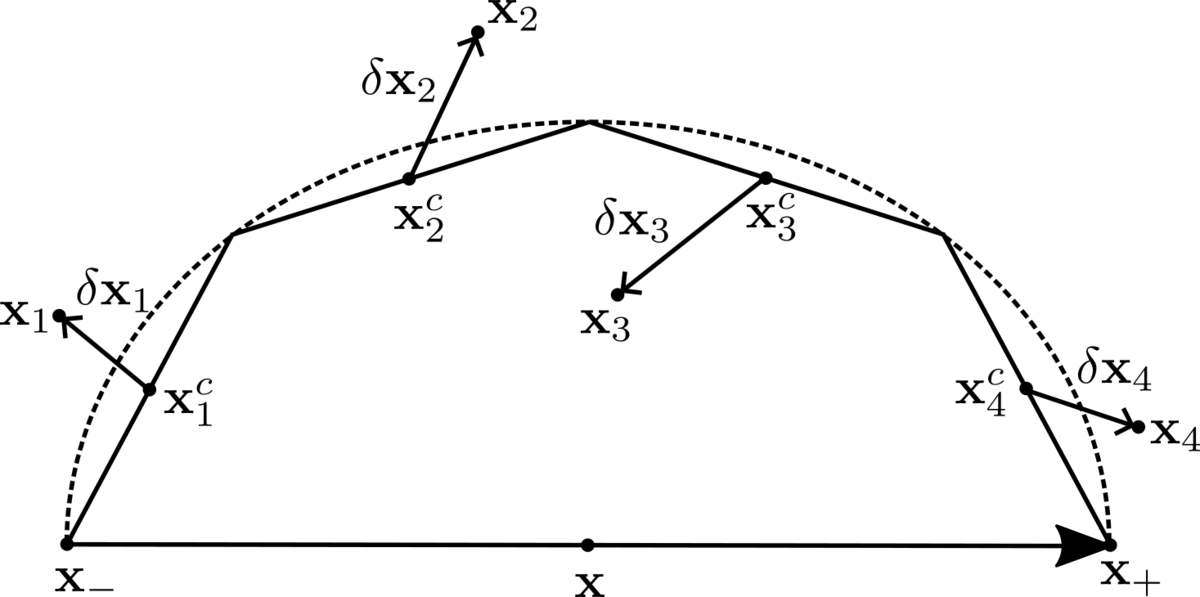
\includegraphics[width=.7\textwidth]{Imagens/expansao_em_torno_da_trajetoria_classica.png}
    \centering
    \caption{Expansão da fase em torno de centros $\mathbf{x}_j^c$ de uma corda cujas pontas jazem na trajetória clássica (tracejada).}
    \label{expansão em torno da trajetória clássica}
\end{figure}

A área já é uma função quadrática, de forma que simplesmente a reescrevemos como
\begin{equation}
    \begin{aligned}
        \Delta_{N+1}\left(\mathbf{x},\mathbf{x}_1,\ldots,\mathbf{x}_{N}\right) &=
        \Delta_{N+1}\left(\mathbf{x} ,\mathbf{x}_1^c+\delta\mathbf{x}_1,\ldots,\mathbf{x}_{N}^c+\delta\mathbf{x}_N\right) \\
    &=\Delta_{N+1}\left(\mathbf{x},\mathbf{x}_1^c,\ldots,\mathbf{x}_{N}^c\right) - \sum_{j=1}^N \mathbf{J} \boldsymbol{\xi}_j \cdot \delta\mathbf{x}_j  + \Delta_{N+1}\left(\boldsymbol{0},\delta\mathbf{x}_1,\ldots,\delta\mathbf{x}_N\right)
    \end{aligned}
\end{equation}
sendo utilizada expressão \eqref{variação área} deduzida no apêndice \ref{apendice_area}. Mas, quando $N$ é grande, as cordas tornam-se aproximadamente tangentes à trajetória, e são aproximadas por $\boldsymbol{\xi}_j \approx t \mathbf{J} \nabla H(\mathbf{x}_j^c)/N$, de forma que
\begin{equation}
    \begin{aligned}
        \Delta_{N+1}\left(\mathbf{x},\mathbf{x}_1,\ldots,\mathbf{x}_{N}\right) &\approx \Delta_{N+1}\left(\mathbf{x},\mathbf{x}_1^c,\ldots,\mathbf{x}_{N}^c\right) \\ &+ \frac{t}{N}\sum_{j=1}^N \nabla H(\mathbf{x}_j^c) \cdot \delta\mathbf{x}_j  + \Delta_{N+1}\left(\boldsymbol{0},\delta\mathbf{x}_1,\ldots,\delta\mathbf{x}_N\right).
    \end{aligned}
\end{equation}

Além disso, inserindo a expansão de segunda ordem para a hamiltoniana
\begin{equation}
    H(\mathbf{x}_j) \approx H\left(\mathbf{x}_j^c\right) + \nabla H \left(\mathbf{x}_j^c\right) \cdot  \delta \mathbf{x}_j + \frac{1}{2} \delta \mathbf{x}_j \cdot \boldsymbol{\mathcal{H}}_{\mathbf{x}^c_j} \delta \mathbf{x}_j,
\end{equation}
obtemos
\begin{equation}
    \begin{aligned}
        U_t \left( \mathbf{x} \right)_{SC} = \exp &\left[ \frac{i}{\hbar} S_t \left(\mathbf{x} \right) \right] \lim_{N \to \infty} \frac{1}{\left( \pi \hbar \right)^{Nd}} \int  \prod_{j=1}^{N} d \mathbf{x}_j \left| \det \left( \mathbf{I} \pm \mathbf{JB}_j \right) \right|^{1/2}  \\ &\times \exp \left[ \frac{i}{\hbar} \Delta_{N+1}\left(\boldsymbol{0},\delta\mathbf{x}_1,\ldots,\delta\mathbf{x}_N\right) - \frac{t}{2N \hbar}\sum_{j=1}^{N} \delta \mathbf{x}_j \cdot \boldsymbol{\mathcal{H}}_{\mathbf{x}^c_j} \delta \mathbf{x}_j \right],
    \end{aligned}
\end{equation}
sendo $S_t$ a ação, como dada em \eqref{ação}. Se também aproximarmos
\begin{equation}
    \mathbf{B}_j \approx - \frac{t}{2N} \boldsymbol{\mathcal{H}}_{\mathbf{x}^c_j},
\end{equation}
o que é consistente com a aproximação de fase estacionária, e realizarmos a mudança de coordenadas $\mathbf{x} \mapsto \delta\mathbf{x}$, cujo determinante jacobiano é $1$, a integral se torna idêntica àquela da fórmula \eqref{composição metapletica}. Para avaliar esse termo, observamos que estamos compondo operadores metapleticos cuja matriz matriz simplética correspondente é uma aproximação linear para o fluxo clássico gerado por $S_{t/N}$. No limite, obtemos então uma aproximação linear para o fluxo gerado por $S_{t}$, cuja matriz simétrica correspondente é $\frac{1}{2} \partial^2 S_t/ \partial \mathbf{x}^2$ o que, recorrendo a \eqref{composição metapletica} avaliada em $\mathbf{x} = \boldsymbol{0}$, nos dá
\begin{equation}
    \label{aproximação semiclássica}
    \begin{aligned}
        U_t\left( \mathbf{x} \right)_{SC} &= \left|\det \left( \mathbf{I} \pm \frac{1}{2} \frac{\partial^2 S_t}{\partial \mathbf{x}^2}\right) \right|^{1/2} \exp \left[ \frac{i}{\hbar} S_t \left(\mathbf{x} \right) \right] \\
         &=  \frac{2^d}{\left|\det \left( \mathbf{I} + \mathbf{M}_t\right) \right|^{1/2}} \exp \left[ \frac{i}{\hbar} S_t \left(\mathbf{x} \right) \right].
    \end{aligned},
\end{equation}
onde denotamos
\begin{equation}
    \mathbf{M}_t = \dfrac{\partial \mathbf{x}_+}{\partial \mathbf{x}_-} = \frac{\partial \boldsymbol{\Phi}_t}{\partial \mathbf{x}} \eval_{\mathbf{x}_-},
\end{equation}
sendo $\boldsymbol{\Phi}_t$ o fluxo hamiltoniano, definido em \eqref{definição fluxo hamiltoniano}.

A fórmula \eqref{aproximação semiclássica}, entretanto, só é válida para tempos suficientemente curtos, quando podemos assegurar a inexistência de cáusticas, que, como é possível ver, constituem singularidades da aproximação. Em geral, após o cruzamento de cáusticas, diversas trajetórias clássicas satisfazem o princípio variacional, e também contribuem para a avaliação do propagador por fase estacionária, nos dando uma fórmula
\begin{equation}
    \label{aproximação semiclássica v2}
    \begin{aligned}
        U_t\left( \mathbf{x} \right)_{SC} &= \sum_j \left|\det \left( \mathbf{I} \pm \frac{1}{2} \frac{\partial^2 S^{(j)}_t}{\partial \mathbf{x}^2}\right) \right|^{1/2} \exp \left[ \frac{i}{\hbar} S^{(j)}_t \left(\mathbf{x} \right) +i \gamma_j \right] \\
         &= \sum_j   \frac{2^d}{\left|\det \left( \mathbf{I} + \mathbf{M}_t^{(j)}\right) \right|^{1/2}}\exp \left[ \frac{i}{\hbar} S^{(j)}_t \left(\mathbf{x} \right) +i \gamma_j\right],
    \end{aligned}
\end{equation}
sendo $j$ um índice que percorre todas as trajetórias relevantes e $\gamma_j$ uma fase relativa entre cada ramo do propagador semiclássico — o índice de Maslov — que quando temos diversos ramos, se torna relevante. A determinação de $\gamma_j$ para a representação de Weyl-Wigner pode ser encontrada em \cite{de2014metaplectic}.

\chapter{O ensemble canônico quântico no espaço de fase}
\label{O ensemble canônico quântico no espaço de fase}

A mecânica estatística clássica no ensemble canônico é caracterizada por uma distribuição de probabilidades — a distribuição de Boltzmann — definida por
\begin{equation}
    P_\beta \left( \mathbf{x} \right) = \frac{1}{Z_c} \exp \left[ - \beta H_c \left( \mathbf{x} \right) \right]
\end{equation}
onde $\beta = 1/kT$, sendo $k$ a constante de Boltzmann e $T$ a temperatura, $H_c\left( \mathbf{x} \right)$ é a hamiltoniana deste sistema clássico e 
\begin{equation}
    Z_c = \int d \mathbf{x} \exp \left[ - \beta H_c \left( \mathbf{x} \right) \right]
\end{equation}
é a função de partição clássica. As médias das variáveis dinâmicas $A_c(\mathbf{x})$ são dadas então por
\begin{equation}
    \ev{A_c}_\beta = \int d \mathbf{x} \ P_\beta \left( \mathbf{x} \right) A_c\left( \mathbf{x} \right)  .
\end{equation}

Já a visão quântica deste problema é, em um primeiro momento, completamente distinta. O sistema é agora caracterizado por um operador hamiltoniano $\hat{H}$ e pelo operador densidade térmico
\begin{equation}
    \hat{\rho}_\beta = \frac{1}{Z} e^{ -\beta \hat{H} },
\end{equation}
onde a função de partição quântica $Z$ é dada por
\begin{equation}
    Z = \Tr e^{ -\beta \hat{H} },
\end{equation}
enquanto os valores esperados de observáveis, que são caracterizados por operadores $\hat{A}$, são calculados como
\begin{equation}
\label{valor esperado quantico}
    \ev{\hat{A}}_\beta = \Tr \hat{A} \hat{\rho}_\beta = \frac{\Tr \hat{A} e^{ -\beta \hat{H} } }{\Tr e^{ -\beta \hat{H} }}.
\end{equation}

Apesar desta diferença conceitual entre as visões clássica e quântica do ensemble canônico, foi com o objetivo de aproximá-las que Wigner introduziu o seu formalismo \cite{PhysRev.40.749}. De fato, utilizando \eqref{traço wigner}, temos
\begin{equation}
\label{partição wigner}
    Z = \frac{1}{\left( 2\pi \hbar \right)^d} \int d\mathbf{x} e^{-\beta \hat{H}} \left( \mathbf{x} \right)
\end{equation}
de forma que a função de Wigner correspondente ao operador densidade térmico é
\begin{equation}
\label{wigner termico}
    W_\beta \left(\mathbf{x}\right) = \frac{e^{-\beta \hat{H}} \left( \mathbf{x} \right)}{\int d\mathbf{x} e^{-\beta \hat{H}} \left( \mathbf{x} \right)}
\end{equation}
e as médias são dadas por
\begin{equation}
\label{valor esperado wigner 2}
    \ev{\hat{A}}_\beta = \int d \mathbf{x} W_\beta(\mathbf{x}) A(\mathbf{x}) = \frac{\int d \mathbf{x} e^{-\beta \hat{H}} \left( \mathbf{x} \right) A(\mathbf{x})}{\int d\mathbf{x} e^{-\beta \hat{H}} \left( \mathbf{x} \right)}
\end{equation}

Apesar das similaridades formais entre o ensemble canônico no formalismo de Wigner e seu correspondente clássico, observamos que diferenças importantes persistem — em geral, $A_c(\mathbf{x})$ não coincide com $A(\mathbf{x})$, embora isso aconteça em casos importantes, mas, de forma mais significativa, $e^{-\beta \hat{H}}(\mathbf{x})$ é diferente de $e^{-\beta H_c(\mathbf{x})}$, especialmente para baixas temperaturas.

Se conhecemos os autoestados $\ket{n}$ da hamiltoniana, bem como os autovalores $E_n$ correspondentes, temos as relações explicitas
\begin{equation}
    \hat{\rho}_\beta = \frac{1}{Z}\sum_{n}e^{-\beta E_n} \ket{n} \bra{n}
\end{equation}
\begin{equation}
\label{partição exata}
    Z = \sum_n e^{-\beta E_n}
\end{equation}
\begin{equation}
\label{valor esperado exato}
    \ev{\hat{A}}_\beta = \dfrac{ \sum_n e^{-\beta E_n}\bra{n}\hat{A}\ket{n} }{\sum_n e^{-\beta E_n} }
\end{equation}

Na maioria dos casos, tais valores não são conhecidos, ou sua obtenção é custosa, sendo então importante o desenvolvimento de métodos alternativos que permitam o cálculo das quantidades termodinâmicas. Neste trabalho, investigamos alguns desses métodos. O ponto de partida é observar que a expressão para o operador de evolução temporal, dada por 
\begin{equation}
    \hat{U}_t = \exp\left( - \frac{it}{\hbar} \hat{H} \right),
\end{equation}
é transformada, se tomarmos um tempo $t = -i\theta$, sendo $\theta = \hbar \beta$ o tempo térmico, em
\begin{equation}
\label{propagador tempo imaginário}
    \hat{U}_{-i\theta} = \exp \left( -\beta \hat{H} \right).
\end{equation}
A ideia é então utilizar a extensão analítica da aproximação semiclássica que desenvolvemos para o operador de evolução temporal para avaliar a símbolo de Wigner de \eqref{propagador tempo imaginário}, o que, por sua vez, nos fornecerá aproximações para \eqref{partição wigner}, \eqref{wigner termico}, \eqref{valor esperado wigner 2}.

Utilizando a fórmula \eqref{aproximação semiclássica}, vemos que a aproximação semiclássica para o símbolo de Wigner de $e^{ -\beta \hat{H}}$ é, em sua forma mais simples, dada por
\begin{equation}
\label{exp beta h semiclassica}
    e^{-\beta \hat{H}}\left( \mathbf{x} \right)_{SC} = \frac{2^d}{\left|\det \left[ \mathbf{I} + \mathbf{M}_{-i\theta}\right] \right|^{1/2} } \exp \left[ \frac{1}{\hbar} S_\theta^{E} \left(\mathbf{x} \right) \right] .
\end{equation}
onde definimos a ação euclidiana $S^{E}_{\theta} = i S_{-i\theta}$ \footnote{O nome vem do fato de que a métrica de Minkowski $ds^2 = -dt^2 + d\mathbf{r}^2$ se transforma, ao introduzir $\theta = -i t$, o que é chamado, nesse contexto, de rotação de Wick, em $ds^2 = d\theta ^2 + d\mathbf{r}^2$, que é uma métrica euclidiana \cite{ingold2002path,greiner2013field}.}, que toma valores reais, pois, como já mencionado, $S_t$ é uma função impar de $t$. Essa fórmula poderia ser deduzida, em analogia com o que fizemos com o propagador, ao escrever
\begin{equation}
    \exp\left( -\beta \hat{H} \right) = \exp\left( -\frac{\beta}{N} \hat{H} \right) \cdots \exp\left( -\frac{\beta}{N} \hat{H} \right)
\end{equation}
utilizar as regras de composição que desenvolvemos na seção \ref{Representação de Weyl-Wigner da composição de operadores}, e, desta vez, avaliar a integral resultante pelo chamado método de \textit{steepest descent} \cite{balian2006microphysics}, que é uma aproximação análoga à aproximação de fase estacionária, embora, nesse caso, seja mais obscura a interpretação do que constituiriam os pontos estacionários da integral correspondente.

Um resultado interessante que já decorre imediatamente de \eqref{exp beta h semiclassica} é que, para tempos pequenos, que correspondem a altas temperaturas, temos $S_t \approx -t H\left(\mathbf{x}\right)$ e $\mathbf{M}_{t} \approx \mathbf{I}$, de forma que
\begin{equation}
\label{limite clássico}
    e^{-\beta \hat{H}}\left( \mathbf{x} \right)_{SC} \approx  \exp \left[ - \beta H\left(\mathbf{x}\right) \right] \approx  \exp \left[ - \beta H_c\left(\mathbf{x}\right) \right],
\end{equation}
isto é, recuperamos a mecânica estatística clássica.

O principal desafio para a aplicação de nossa aproximação semiclássica é o cálculo da ação euclidiana e da amplitude para um sistema arbitrário. Uma solução simples para essa questão consiste em utilizar a aproximação que descrevemos na seção \ref{Expressões Aproximadas}, como discutiremos a seguir. Depois, desenvolveremos uma técnica mais avançada para realizar estes cálculos para sistemas arbitrários.

\section{Ação euclidiana aproximada}
\label{Ações euclidianas aproximadas}

Na seção \ref{Expressões Aproximadas}, descrevemos uma forma de obter aproximações para a ação que se baseava na aproximação do fluxo gerado por uma hamiltoniana arbitrária por aquele gerado por uma expansão desta hamiltoniana em uma série de Taylor até segunda ordem. Isso resultou na expressão \eqref{metapletica_amortecida_real}, que admite uma extensão analítica imediata, nos permitindo a obtenção de uma ação euclidiana
\begin{equation}
    S^E(\mathbf{x},\theta) \approx -\theta H(\mathbf{x}) + \frac{1}{\Omega_\mathbf{x}^2}\left[\frac{\theta}{2}-\frac{1}{\Omega_\mathbf{x}}\tanh \left(\frac{\Omega_\mathbf{x} \theta}{2}\right)\right] \left( \text{adj } \boldsymbol{\mathcal{H}}_\mathbf{x} \right) \mathbf{h}_\mathbf{x} \cdot \mathbf{h}_\mathbf{x}
\end{equation}
Além disso, como já vimos, hamiltonianas quadráticas geram fluxos lineares, de forma que $\mathbf{M}_t$ pode ser aproximado pela expressão \eqref{fluxo linear}, com a diferença que substituímos $\boldsymbol{\mathcal{H}_0}$ por $\boldsymbol{\mathcal{H}_\mathbf{x}}$, o que nos permite calcular 
\begin{equation}
    \mathbf{M}_t = \exp\left( t \mathbf{J} \boldsymbol{\mathcal{H}_\mathbf{x}}\right) = \cos \left( \Omega_\mathbf{x} t\right) \mathbf{I} + \frac{\sin \left( \Omega_\mathbf{x} t\right)}{\Omega_\mathbf{x}} \mathbf{J} \boldsymbol{\mathcal{H}_\mathbf{x}}
\end{equation}
de forma que a amplitude é
\begin{equation}
    \frac{2}{\left|\det \left[ \mathbf{I} + \mathbf{M}_{t}\right] \right|^{1/2} } = \sec \left( \frac{\Omega_\mathbf{x} t}{2} \right),
\end{equation}
expressão esta que também admite uma extensão analítica imediata. Combinando esses resultados obtemos então
\begin{equation}
    \begin{aligned}
        e^{-\beta \hat{H}} \left( \mathbf{x}\right)_{DM} &= \sech \left(\frac{\Omega_\mathbf{x} \theta}{2}\right)\\ &\times \exp \left\{-\beta H(\mathbf{x}) + \frac{1}{\Omega_\mathbf{x}^2}\left[\frac{\beta}{2}-\frac{1}{\hbar\Omega_\mathbf{x}}\tanh \left(\frac{\Omega_\mathbf{x} \theta}{2}\right)\right] \left( \text{adj } \boldsymbol{\mathcal{H}}_\mathbf{x} \right) \mathbf{h}_\mathbf{x} \cdot \mathbf{h}_\mathbf{x}\right\},
    \end{aligned}
\end{equation}
que chamaremos de metaplética amortecida (\textit{dampened metaplectic}) \footnote{Este nome, cunhado em \cite{OZORIODEALMEIDA2021132951}, se deve ao fato de que tal expressão pode ser escrita como a continuação analítica da representação de Wigner de um certo operador localmente metaplético, que ainda é multiplicada por um fator de amortecimento.}. Esta expressão pode ainda ser escrita de forma mais compacta ao introduzir 
\begin{equation}
\label{definição alpha}
    \alpha = \frac{\theta \Omega_{\mathbf{x}}}{2}
\end{equation}
e
\begin{align*}
    f(\alpha) = \begin{cases}
        \dfrac{\tanh(\alpha)}{\alpha}, & \alpha \ne 0 \\
        1, & \alpha = 0
    \end{cases} \ \ \ \ \ \Label{definição f} \ \  g(\alpha) = \begin{cases}
        \dfrac{1-f(\alpha)}{\alpha^2}, & \alpha \ne 0 \\
        \dfrac{1}{3}, & \alpha = 0
    \end{cases} \ \ \ \ \ \Label{definição g}
\end{align*}
de forma que temos
\begin{equation}
\label{aproximação dm}
    e^{-\beta \hat{H}} \left( \mathbf{x}\right)_{DM} = \sech \alpha \exp \left\{ -\beta \left[  H(\mathbf{x}) - \frac{g(\alpha) \theta^2}{8} \left( \text{adj } \boldsymbol{\mathcal{H}}_\mathbf{x} \right) \mathbf{h}_\mathbf{x} \cdot \mathbf{h}_\mathbf{x} \right] \right\}.
\end{equation}
Notamos que, quando $\det \boldsymbol{\mathcal{H}}_\mathbf{x} < 0$, $\alpha$ torna-se imaginário, embora $f(\alpha)$ e $g(\alpha)$ permaneçam reais. Os gráficos dessas funções podem ser vistos na figura \eqref{f e g total}.

\begin{figure}[H]
     \centering
     \begin{subfigure}[b]{0.48\textwidth}
         \centering
         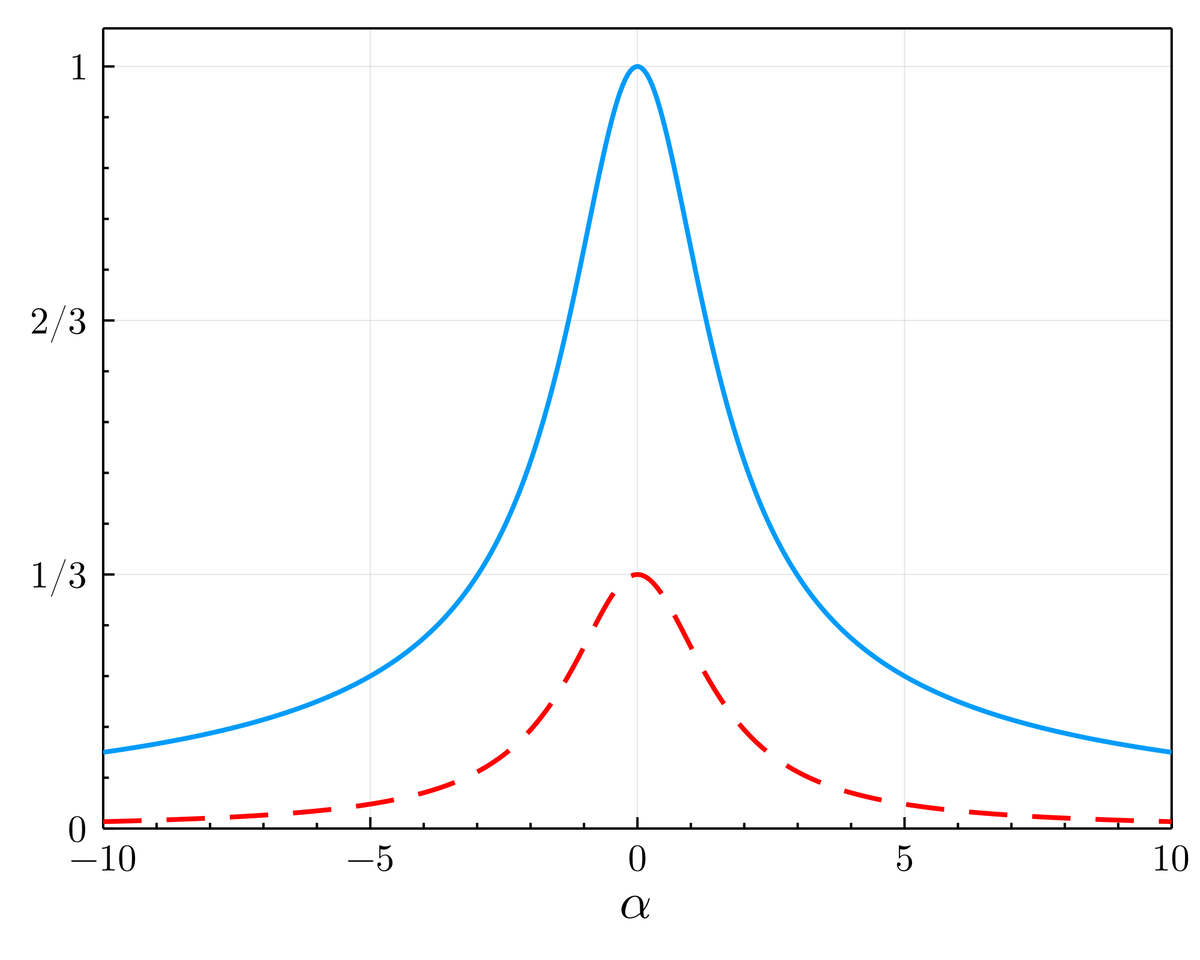
\includegraphics[width=\textwidth]{Imagens/fg.png}
         \caption{Linha azul cheia: $f(\alpha)$. Linha vermelha pontilhada: $g(\alpha)$}
         \label{f e g}
     \end{subfigure}
     \hfill
     \begin{subfigure}[b]{0.48\textwidth}
         \centering
         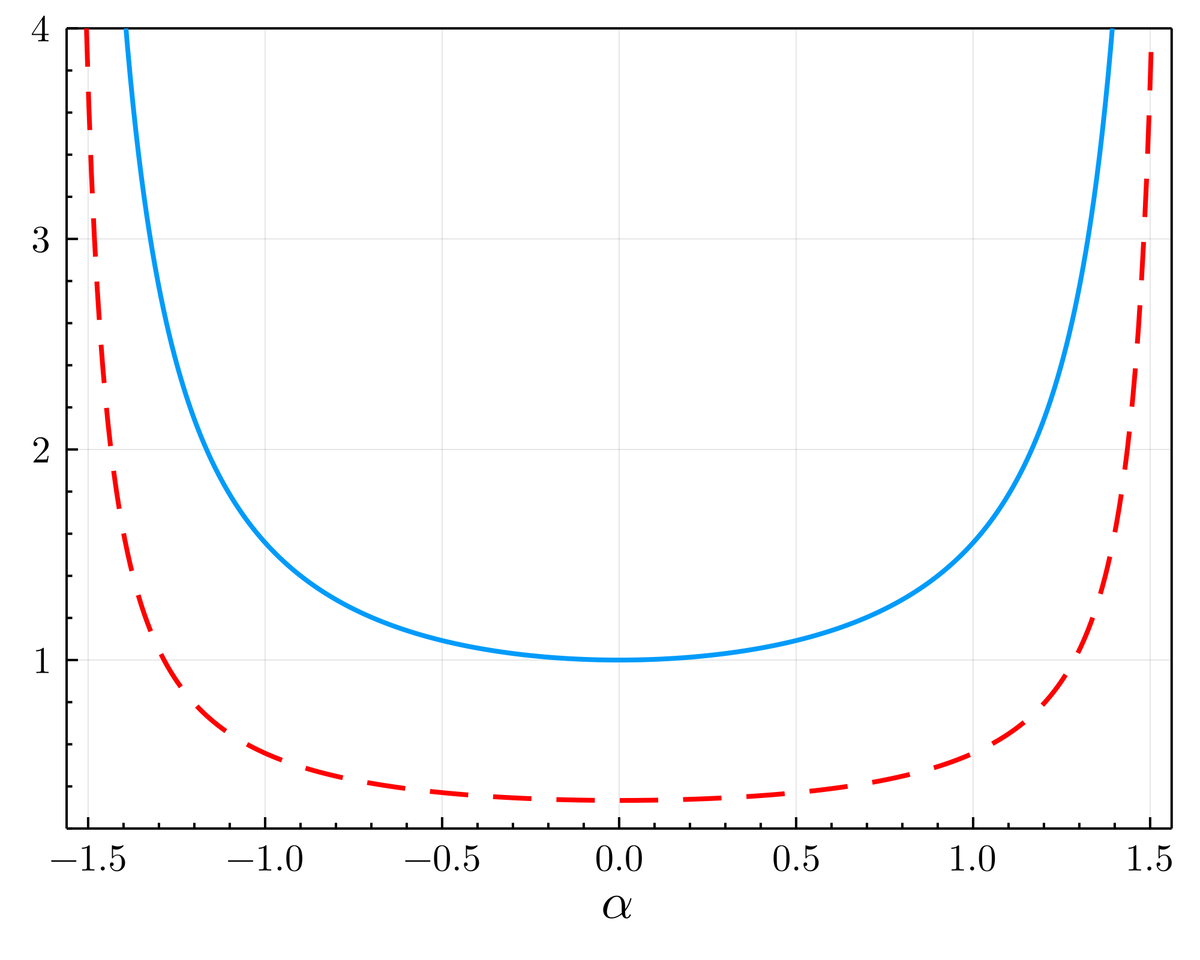
\includegraphics[width=\textwidth]{Imagens/fgi.png}
         \caption{Linha azul cheia: $f(i\alpha)$. Linha vermelha pontilhada: $g(i\alpha)$}
         \label{fi e gi}
     \end{subfigure}
     \caption{Gráficos de $f$ e $g$ para argumentos reais e puramente imaginários.}
        \label{f e g total}
\end{figure}

É interessante notar que, ao tomar $\hbar \to 0$, temos $\alpha \to 0$, e a aproximação tende a $\exp\left[-\beta H(\mathbf{x}) \right]$, que, a menos da possível diferença entre $H(\mathbf{x})$ e $H_c(\mathbf{x})$, é precisamente o resultado clássico, como em \eqref{limite clássico}.

\section{A aproximação semiclássica completa}

\subsection{Uma mudança de coordenadas}
\label{Uma mudança de coordenadas}

Antes de obter explicitamente as quantidades necessárias para a aproximação semiclássica das médias termodinâmicas, será conveniente apontar alguns problemas na sua aplicação imediata, e, em seguida, proporemos uma simples solução.

Como já vimos, as médias termodinâmicas são calculadas como a razão de dois traços, como dado em \eqref{valor esperado quantico}. Logo, na aproximação semiclássica, seu cálculo se reduz ao cálculo de integrais da forma
\begin{equation}
\label{valor esperado importante}
    \Tr \hat{U}_t \hat{A} \approx \frac{1}{(2\pi \hbar)^d}\int \frac{2^dd \mathbf{x}}{\left|\det \left[ \mathbf{I} + \mathbf{M}_{t}\right] \right|^{1/2} } \exp \left[ \frac{i}{\hbar} S_t \left(\mathbf{x} \right) \right] A(\mathbf{x}).
\end{equation}
A aplicação direta dessa expressão é um tanto inconveniente, pois as trajetórias clássicas relevantes são definidas implicitamente pelo seu centro $\mathbf{x}$ e, além disso, 
o integrando torna-se singular nas cáusticas. Esses problemas são resolvidos de forma simples ao trocar a variável de integração para o ponto médio da trajetória, como descrito pelas equações \eqref{não sei dar nomeee} e \eqref{problema valor inicial}, sendo então a ação calculada através de \eqref{ação conveniente}.

O jacobiano desta transformação é dado por
\begin{equation}
    \frac{\partial \mathbf{x}}{\partial \mathbf{X}}(\mathbf{X},t/2) = \frac{1}{2}\left(\mathbf{M}_{t/2}\left( \mathbf{X} \right) + \mathbf{M}_{-t/2}\left( \mathbf{X} \right) \right),
\end{equation}
e, além disso, valem $\mathbf{M}_{t/2}(\mathbf{x}_-) =  \left[ \mathbf{M}_{-t/2}\left( \mathbf{X}     \right) \right]^{-1}$, $\det \mathbf{M}_{t/2}(\mathbf{x}_-) = 1$ e $\mathbf{M}_{t/2}\left(\mathbf{X}     \right)\mathbf{M}_{t/2}\left(\mathbf{x}_- \right) = \mathbf{M}_{t}\left(\mathbf{x}_- \right)$. Desta forma, temos
\begin{equation}
    \left| \det\frac{ \partial \mathbf{x}}{\partial \mathbf{X}}(t/2) \right| = \frac{1}{2^{2d}} \left|\det \left[ \mathbf{I} + \mathbf{M}_{t}\left(\mathbf{x}_- \right)\right] \right|,
\end{equation}
e, então,
\begin{equation}
\label{valor esperado importante 2}
    \Tr \hat{U}_t \hat{A} = \frac{1}{(2\pi \hbar)^d}\int d \mathbf{X}  \left|\det \frac{\partial \mathbf{x}}{\partial \mathbf{X}} \right|^{1/2} \exp \left[ \frac{i}{\hbar} S_t \left(\mathbf{x} \right) \right] A(\mathbf{x} ),
\end{equation}
sendo $\mathbf{x}$ e $\partial \mathbf{x}/\partial \mathbf{X}$ avaliados em $\left(\mathbf{X},t/2 \right)$. Vemos que esta expressão não possui singularidades, e as trajetórias necessárias para o cálculo do integrando são agora definidas a partir do problema de valor inicial \eqref{problema valor inicial}.

\subsection{Espaço de fase duplo e sua complexificação}

Nessa seção, descreveremos um método que permite, numericamente, a obtenção de todos os termos do integrando \eqref{valor esperado importante 2} para um sistema arbitrário e para um valor qualquer de $t \in \mathbb{C}$, o que nos permitirá aplicar as aproximações semiclássicas para o ensemble canônico a uma enorme quantidade de casos.

Para compreender o problema que nos é posto, é conveniente, por enquanto, focar a nossa análise na realização da continuação analítica da ação $S$. O termo problemático em \eqref{ação} é a área 
\begin{equation}
    \Delta\left[ \mathbf{x}\left( \mathbf{X}\right),t \right] = \int_0^{t/2} \boldsymbol{\xi}\left(\mathbf{X}, t' \right) \wedge \dot{\mathbf{x}}\left(\mathbf{X}, t' \right) dt',
\end{equation}
entre a corda e a trajetória, já que estaremos interessados apenas em hamiltonianas independentes do tempo. Ao invés de obter essas quantidades indiretamente ao evoluir uma trajetória para frente e outra para trás, e em seguida realizar as combinações em \eqref{problema valor inicial}, podemos obtê-las diretamente a partir de uma única trajetória de um sistema hamiltoniano definido sobre um espaço de fase duplicado. Nesse novo espaço, $\mathbf{x}$ faz o papel de posição dupla, cujo momento duplo associado é $\mathbf{y} = \mathbf{J}\boldsymbol{\xi}$, enquanto as equações de movimento dessas variáveis são geradas pela hamiltoniana dupla
\begin{equation}
    \mathbb{H}(\mathbf{x},\mathbf{y}) = H\left( \mathbf{x} - \frac{1}{2}\mathbf{J} \mathbf{y} \right) + H\left( \mathbf{x} + \frac{1}{2}\mathbf{J} \mathbf{y} \right) = H(\mathbf{x}_+) + H(\mathbf{x}_-).
\end{equation}
De fato, temos
\begin{subequations}
\label{equações de movimento espaço de fase duplo}
    \begin{equation}
    \frac{\partial \mathbb{H}}{\partial \mathbf{x}} = \nabla H(\mathbf{x}_+) + \nabla H(\mathbf{x}_-) = -\mathbf{J} \left( \dot{\mathbf{x}}_+-\dot{\mathbf{x}}_- \right) = -\mathbf{J} \dot{\boldsymbol{\xi}} = -\dot{\mathbf{y}}
    \end{equation}
    \begin{equation}
    \frac{\partial \mathbb{H}}{\partial \mathbf{y}} = \frac{\mathbf{J}}{2}\left[\nabla H(\mathbf{x}_+) - \nabla H(\mathbf{x}_-)\right] = \frac{1}{2}\left( \dot{\mathbf{x}}_++\dot{\mathbf{x}}_- \right) =  \dot{\mathbf{x}},
\end{equation}
\end{subequations}
enquanto as condições iniciais correspondentes são
\begin{equation}
\label{condições iniciais}
    \mathbf{x}\left( \mathbf{X},0 \right) = \mathbf{X}, \ \ \ \mathbf{y}\left( \mathbf{X},0 \right) = \boldsymbol{0}.
\end{equation}
Em termos de $\mathbf{x}$ e $\mathbf{y}$ e $\mathbb{H}$, a ação toma então a forma padrão
\begin{equation}
    S\left(t,\mathbf{x}\left(\mathbf{X} \right) \right) = \int_0^{t/2}  \mathbf{y}\left( t'\right) \cdot \dot{\mathbf{x}}\left( t' \right) dt' - \frac{t}{2} \mathbb{H}\left(\mathbf{X},\mathbf{0} \right).
\end{equation}

Vemos que, para calcular $S$ em tempos complexos, temos que, de alguma forma, ser capazes de obter $\mathbf{x}$ e $\mathbf{y}$ para argumentos complexos. Como essas quantidades são definidas pelas equações diferenciais \eqref{equações de movimento espaço de fase duplo} em conjunto com as condições iniciais \eqref{condições iniciais}, nossa proposta para extendê-las a todo plano complexo é simplesmente promover as derivadas temporais em \eqref{equações de movimento espaço de fase duplo} a derivadas em relação a uma variável complexa $z$, de forma que
\begin{equation}
    \begin{aligned}
        \dfrac{d \mathbf{y}}{dz} &= -\dfrac{\partial \mathbb{H}}{\partial \mathbf{x}} \\
        \dfrac{d \mathbf{x}}{dz} &= \dfrac{\partial \mathbb{H}}{\partial \mathbf{y}}
    \end{aligned}
\end{equation}
enquanto mantemos as condições iniciais. Se $\mathbb{H}$ for bem comportada, obtemos então funções que são analíticas em todo $\mathbb{C}$, e integrais de linha envolvendo $\mathbf{x}$ e $\mathbf{y}$ dependem apenas dos pontos finais do caminho considerado. Assim sendo, para calcular essas quantidades em um ponto $z \in \mathbb{C}$ qualquer, propomos o seguinte procedimento — consideramos o caminho mais simples que liga a origem a $z$ — o segmento de reta. Uma possível parametrização desse caminho é feita ao introduzir o número $w = z/|z|$ e a função
\begin{align*}
  \gamma \colon[0,|z|] &\to \mathbb{C}\\
  s &\mapsto  s w,
\end{align*}
de forma que $s$ é distância entre a origem e o ponto $\gamma(s)$ — isto é, fazemos uma parametrização pelo comprimento de arco. Este caminho é ilustrado na figura \ref{plano complexo}. Agora, compomos $\mathbf{x}$ e $\mathbf{y}$ com $\gamma$, isto é, definimos as funções $\tilde{\mathbf{x}}:[0,|z|]\to \mathbb{C}, \ \tilde{\mathbf{x}}(s) = \mathbf{x}\circ \gamma(s) = \mathbf{x}(sw)$ e $\tilde{\mathbf{y}}:[0,|z|]\to \mathbb{C}, \ \tilde{\mathbf{y}}(s) = \mathbf{y}\circ \gamma(s) = \mathbf{y}(sw)$. 
\begin{figure}[H]
    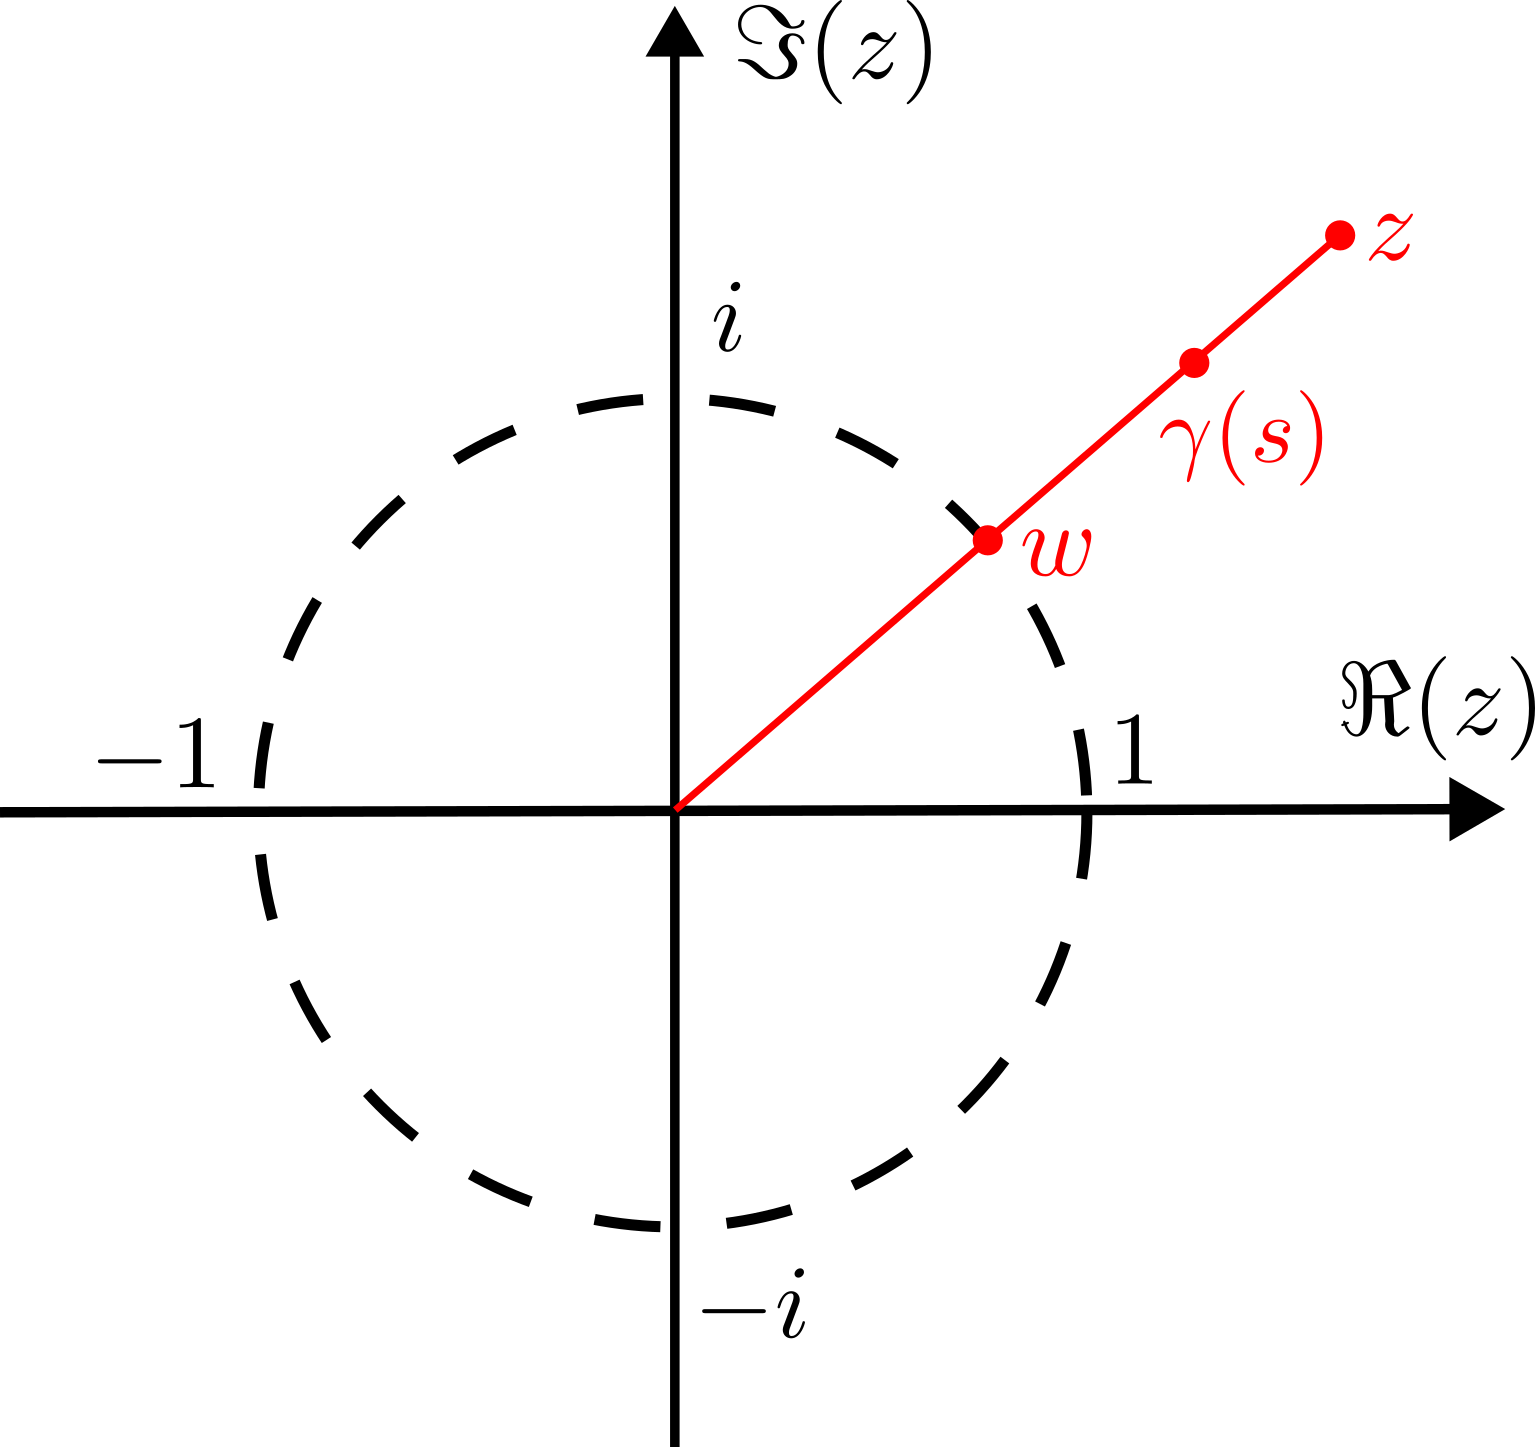
\includegraphics[width=.5\textwidth]{Imagens/plano_complexo.png}
    \centering
    \caption{Segmento de reta unindo a origem a um ponto $z$.}
    \label{plano complexo}
\end{figure}

Utilizando a regra da cadeia, concluímos que essas funções satisfazem a EDO
\begin{equation}
    \begin{aligned}
        \dfrac{d \tilde{\mathbf{y}}}{ds} &= -w\dfrac{\partial \mathbb{H}}{\partial \mathbf{x}} \\
        \dfrac{d \tilde{\mathbf{x}}}{ds} &= w\dfrac{\partial \mathbb{H}}{\partial \mathbf{y}} 
    \end{aligned},
\end{equation}
e, ao definir a quantidade $\tilde{\mathbf{y}}_w = w^* \tilde{\mathbf{y}}$, onde $^*$ denota o complexo conjugado, e a hamiltoniana modificada
\begin{equation}
    \mathbb{H}_{w}\left(\mathbf{x},\mathbf{y}\right) =  \mathbb{H}\left(\mathbf{x},w\mathbf{y}\right) = H\left( \mathbf{x} - \frac{w}{2}\mathbf{J} \mathbf{y} \right) + H\left( \mathbf{x} + \frac{w}{2}\mathbf{J} \mathbf{y} \right),
\end{equation}
recuperamos equações de Hamilton
\begin{equation}
    \begin{aligned}
        \dfrac{d \tilde{\mathbf{y}}_w}{ds} &= -\dfrac{\partial \mathbb{H}_{w}}{\partial \mathbf{x}} \\
        \dfrac{d \tilde{\mathbf{x}}}{ds} &= \dfrac{\partial\mathbb{H}_{w}}{\partial \mathbf{y}}
    \end{aligned}
\end{equation}
com uma hamiltoniana em geral complexa, mas que se reduz a uma função real se $w \in \left\{ 1,-1,i,-i \right\}$.

Agora, para calcular $\Delta(z)$, também temos a liberdade de escolher qualquer caminho que ligue $0$ a $z/2$. Escolhendo novamente o segmento de reta, obtemos
\begin{equation}
\label{formula integral área}
    \begin{aligned}
        \Delta(z) &= \int_\gamma \mathbf{y}(z') \cdot \frac{d\mathbf{x}(z')}{dz} dz' \\
        &= \int_{0}^{|z|/2} \tilde{ \mathbf{y}}(s) \cdot \frac{d\tilde{ \mathbf{x}}(s)}{ds} ds \\
        &= w\int_{0}^{|z|/2} ds \ \tilde{ \mathbf{y}}_w(s) \cdot \frac{d\tilde{ \mathbf{x}}(s)}{ds}  \\
        &= w\int_{0}^{|z|/2} ds \ \tilde{ \mathbf{y}}_w(s) \cdot \dfrac{\partial\mathbb{H}_{w}}{\partial \mathbf{y}} \eval_{\tilde{\mathbf{x}}(s),\tilde{\mathbf{y}}_w(s)}.
    \end{aligned}
\end{equation}

\begin{exmp}
    Para nos familiarizarmos com esse formalismo, é conveniente realizar este cálculo para a hamiltoniana
    \begin{equation}
        H(\mathbf{x}) = \frac{1}{2} \mathbf{x}^2
    \end{equation}
    do oscilador harmônico. Nesse caso, a hamiltoniana modificada fica
    \begin{equation}
        \begin{aligned}
            \mathbb{H}_{w}(\mathbf{x},\mathbf{y}) &= \frac{1}{2}\left[ \left( \mathbf{x} - \frac{w}{2}\mathbf{J} \mathbf{y} \right)^2 + \left( \mathbf{x} + \frac{w}{2}\mathbf{J} \mathbf{y} \right)^2 \right] \\
        &= \mathbf{x}^2 + \frac{w^2}{4}\mathbf{y}^2
        \end{aligned}
    \end{equation}
    e as equações de Hamilton são
    \begin{equation}
    \begin{aligned}
        \dfrac{d \tilde{\mathbf{y}}_w}{ds} &= -2\tilde{\mathbf{x}} \\
        \dfrac{d \tilde{\mathbf{x}}}{ds} &= \frac{w^2}{2} \tilde{\mathbf{y}}_w
    \end{aligned}
\end{equation}
o que nos dá uma solução
\begin{equation}
    \begin{aligned}
        \tilde{\mathbf{y}}_w(s) &= \frac{2}{w} \sin\left( ws\right)\mathbf{X} \\
        \tilde{\mathbf{x}}(s) &=  \cos\left( ws\right)\mathbf{X}
    \end{aligned}
\end{equation}
    de forma que obtemos a área
        \begin{equation}
        \begin{aligned}
        \Delta(z) &= w\int_{0}^{|z|/2} \tilde{ \mathbf{y}}_w(s) \cdot \frac{d\tilde{\mathbf{x}}(s)}{ds}  ds \\
        &= 2 \mathbf{X}^2 w \int_{0}^{|z|/2} \sin^2(ws) ds \\
        &= \frac{\mathbf{X}^2}{2} \left[ w|z| - \sin(w|z|) \right] \\
        &= \frac{\mathbf{X}^2}{2} \left[ z - \sin(z) \right],
    \end{aligned}
\end{equation}
que é exatamente o resultado que se obtém ao aplicar o argumento geométrico da seção \ref{Formas Normais}.
\end{exmp}

O nosso interesse reside no caso em que $z = -i \theta$, e, portanto, $w = -i$, de forma que, para abreviar a notação, omitiremos os subscritos $w$, bem como o $\sim$ sobre $\mathbf{x}$ e $\mathbf{y}$, e trocaremos o parâmetro $s$ por $\theta$.

Estamos então quase prontos para calcular as médias termodinâmicas. Revisando o que temos até agora, a dinâmica de $\mathbf{x}$ e $\mathbf{y}$ é dada pelas equações de Hamilton
\begin{subequations}
\label{hamilton térmico}
    \begin{equation}
        \frac{d \mathbf{y}}{d\theta} = -\frac{\partial\mathbb{H}}{\partial \mathbf{x}}, \ \ \ \mathbf{y}(0) = \boldsymbol{0}
    \end{equation}
    \begin{equation} 
        \frac{d \mathbf{x}}{d\theta} = \frac{\partial\mathbb{H}}{\partial \mathbf{y}}, \ \ \ \mathbf{x}(0) = \mathbf{X}
    \end{equation}
\end{subequations}
geradas por uma hamiltoniana modificada
\begin{equation}
    \mathbb{H}(\mathbf{x},\mathbf{y}) = H\left( \mathbf{x} + \frac{i}{2}\mathbf{J} \mathbf{y} \right) + H\left( \mathbf{x} - \frac{i}{2}\mathbf{J} \mathbf{y} \right).
\end{equation}
Já a área euclidiana $\Delta^E(\theta) = i\Delta(-i\theta)$, satisfaz
\begin{equation}
\label{área térmica}
    \frac{d \Delta^E}{d \theta} = \mathbf{y} \cdot  \frac{\partial\mathbb{H}}{\partial \mathbf{y}}, \ \ \ \ \ \Delta^E (0) = 0,
\end{equation}
expressão esta que decorre de \eqref{formula integral área} e constitui um problema de valor inicial que pode ser resolvido concomitantemente com \eqref{hamilton térmico}. Precisamos ainda do jacobiano $\partial \mathbf{x}/ \partial \mathbf{X}$, que pode ser obtido ao tomar as derivadas de \eqref{hamilton térmico} em relação a $\mathbf{X}$, o que nos fornece as equações
\begin{subequations}
\label{jacobianos}
    \begin{equation}
        \frac{d}{d\theta} \frac{\partial \mathbf{y}}{\partial \mathbf{X}} = - \frac{\partial^2\mathbb{H}}{\partial \mathbf{x} \partial \mathbf{y}}\frac{\partial \mathbf{y}}{\partial \mathbf{X}} - \frac{\partial^2\mathbb{H}}{\partial \mathbf{x}^2}\frac{\partial \mathbf{x}}{\partial \mathbf{X}}, \ \ \ \ \ \frac{\partial \mathbf{y}}{\partial \mathbf{X}}\biggr|_{\theta = 0} = \boldsymbol{0}
    \end{equation}
    \begin{equation}
        \frac{d}{d\theta} \frac{\partial \mathbf{x}}{\partial \mathbf{X}} = \frac{\partial^2\mathbb{H}}{\partial \mathbf{y}^2}\frac{\partial \mathbf{y}}{\partial \mathbf{X}} + \frac{\partial^2\mathbb{H}}{\partial \mathbf{x} \partial \mathbf{y}}\frac{\partial \mathbf{x}}{\partial \mathbf{X}} , \ \ \ \ \  \eval{\frac{\partial \mathbf{x}}{\partial \mathbf{X}}}_{\theta = 0} = \mathbf{I},
    \end{equation}
\end{subequations}
que representam mais um problema de valor inicial acoplado a \eqref{hamilton térmico}, envolvendo também $\partial \mathbf{y}/\partial \mathbf{X}$.

Logo, o valor esperado de um operador $\hat{A}$ no ensemble canônico, que é dado, na aproximação semiclássica, por
\begin{equation}
\label{aproximação semiclassica termica}
    \ev{\hat{A}}_\beta \approx \frac{1}{Z_\beta} \int d \mathbf{X} \left| \det \frac{\partial \mathbf{x}}{\partial \mathbf{X}} \right|^{1/2} \exp \left[ \frac{\Delta^E}{\hbar} - \beta H\left( \mathbf{X}\right) \right] A \left( \mathbf{x} \right),
\end{equation}
fica determinado a partir da solução dos problemas de valor inicial especificados por \eqref{hamilton térmico}, \eqref{área térmica} e \eqref{jacobianos}, propagados até um tempo térmico $\theta = \beta \hbar/2$.

\chapter{Aproximação semiclássica para as formas normais}
\label{Dinâmica gerada por formas normais}

Como um primeiro teste para as nossas aproximações semiclássicas, seria interessante aplicá-las a um sistema para o qual seja possível encontrar uma expressão exata para a ação euclidiana, de forma que não seja necessária a obtenção numérica de trajetórias. Uma boa família de candidatos será então sistemas cujo operador hamiltoniano toma a forma
\begin{equation}
\label{operador forma normal}
    \hat{H} = G \left( \frac{\hat{p}^2+\hat{q}^2}{2} \right),
\end{equation}
sendo $G$ um polinômio. Os autoestados $\ket{n}$ desse sistema são os mesmos do oscilador harmônico, enquanto as autoenergias correspondentes são $E_n = G\left[\hbar\left(n+1/2 \right) \right]$, o que também torna imediato o cálculo de médias termodinâmicas exatas a partir da expressão \eqref{valor esperado exato}, de forma que teremos um parâmetro com o qual comparar as aproximações semiclássicas. Para seu cálculo, é necessário encontrar a símbolo de Wigner de $\hat{H}$, que, como mostrado no apêndice \ref{Símbolo de Wigner para formas normais}, pode ser escrito como
\begin{equation}
     H(p,q) = F \left( \frac{p^2+q^2}{2} \right),
\end{equation}
onde $F$ é um outro polinômio, que, a menos no caso do oscilador harmônico, difere de $G$. Em outras palavras, o símbolo de Wigner de $\hat{H}$ está na forma normal de Birkhoff.

\section{Análise das aproximações}
\subsection{Aproximação Metapletica Amortecida}

Essa aproximação pode ser calculada ao substituir as fórmulas \eqref{formulas metapleticas} nos resultados discutidos na seção \ref{Ações euclidianas aproximadas}, de onde obtemos
\begin{equation}
    e^{-\beta \hat{H}} \left( \mathbf{x}\right)_{DM} = \sech \alpha \exp \left\{ -\beta \left[  F(J) - \frac{g(\alpha) \theta^2 J \omega^3(J)}{4}\right] \right\},
\end{equation}
sendo
\begin{equation}
    \alpha = \frac{\theta}{2} \sqrt{\omega(J)\left[\omega(J) + 2J \omega'(J)\right]}
\end{equation}
e $g$ definido em \eqref{definição g}.

\subsection{Aproximação Semiclássica Completa}

Nesse caso, podemos recorrer às expressões \eqref{ação real forma normal}, \eqref{centro real forma normal} e \eqref{det jac real forma normal}, que admitem uma extensão analítica imediata. Obtemos então uma ação euclidiana
\begin{equation}
\label{ação euclidiana}
    S_\theta^E\left[ \mathbf{x}\left( \mathbf{X}\right) \right] = \left[ \omega \theta - \sinh \left(\omega \theta\right) \right] J - \theta F\left( J \right),
\end{equation}
um centro
\begin{equation}
\label{centro térmico}
    \mathbf{x}\left( \mathbf{X},-i\theta/2 \right) = \cosh \left (\frac{\omega \theta}{2} \right) \mathbf{X},
\end{equation}
e um determinante jacobiano
\begin{equation}
\label{jacobiano tempo imaginário}
    \det \frac{\partial \mathbf{x}}{\partial \mathbf{X}}(\mathbf{X},-i\theta/2) = \cosh^2 \left( \frac{\omega \theta}{2} \right)\left[1 + J \omega'  \theta \tanh \left( \frac{\omega \theta}{2} \right) \right],
\end{equation}
que são todos os elementos necessários para calcular a aproximação semiclássica \eqref{aproximação semiclassica termica}. A função de partição fica
\begin{equation}
    \begin{aligned}
        Z_\beta = \Tr \hat{U}_{-i\theta} = \frac{1}{2\pi \hbar}\int d^2 \mathbf{X}  &\cosh \left( \frac{\omega \theta}{2} \right)\sqrt{\left|1 + J \omega'  \theta \tanh \left( \frac{\omega \theta}{2} \right)\right|}\\  \times &\exp \left[ \frac{1}{\hbar} \left\{ \left[ \omega \theta - \sinh \left(\omega \theta\right) \right] J - \theta F\left( J \right) \right\} \right] 
    \end{aligned}
\end{equation}
enquanto os valores esperados de observáveis são
\begin{equation}
    \begin{aligned}
        \ev{\hat{A}}_\beta = \frac{1}{Z_\beta}\Tr \hat{U}_{-i\theta} \hat{A} = \frac{1}{2\pi \hbar Z}\int d^2 \mathbf{X}  &\cosh \left( \frac{\omega \theta}{2} \right)\sqrt{\left|1 + J \omega'  \theta \tanh \left( \frac{\omega \theta}{2} \right)\right|}\\  \times &\exp \left[ \frac{1}{\hbar} \left\{ \left[ \omega \theta - \sinh \left(\omega \theta\right) \right] J - \theta F\left( J \right) \right\} \right] \\ &\times A \left[ \cosh \left (\frac{\omega \theta}{2} \right) \mathbf{X} \right]
    \end{aligned}
\end{equation}
Notamos ainda que, para a função de partição, ou para observáveis tais que $A(\mathbf{x})$ possa ser escrito como uma função de $\mathbf{x}^2$, é conveniente realizar a mudança de variáveis $\mathbf{X}=\left(\sqrt{2J}\cos \phi,\sqrt{2J}\sin\phi\right)$, que satisfaz $d^2 \mathbf{X} = dJ d\phi$, de forma que a integral sobre $\phi$ é trivialmente feita, restando apenas uma integral simples sobre $J$.

É instrutivo analisar o comportamento de nossa aproximação no limite de baixas temperaturas. Tomando o quadrado de $\eqref{centro térmico}$, temos
\begin{equation}
\label{J em função de x}
    \frac{\mathbf{x}^2}{2} = J \cosh^2 \left[ \frac{\theta \omega\left(J\right)}{2} \right].
\end{equation}
Interpretando essa expressão como definindo implicitamente $J\left( \mathbf{x},\theta \right)$, vemos que, fixado $\mathbf{x}$, para que o lado direito da igualdade permaneça finito, devemos ter 
\begin{equation}
    \lim_{\theta \to \infty} J\left( \mathbf{x},\theta \right) = 0 \text{ ou } \lim_{\theta \to \infty} \omega \left[ J\left( \mathbf{x},\theta \right) \right] = 0.
\end{equation}
Logo, para sistemas que satisfazem $\omega \left( J \right) \ne 0 \ \forall \ J$, vemos que, de acordo com \eqref{J em função de x}, $J$ tem o comportamento assintótico
\begin{equation}
    J \approx \frac{\mathbf{x}^2}{2} \sech^2 \left[ \frac{\theta \omega\left(0\right)}{2} \right], \ \ \ \theta \omega\left(0\right) \gg 1
\end{equation}

Substituindo esta expressão em \eqref{ação euclidiana} e tomando o limite $\theta \to \infty$, obtemos, a menos de um termo constante em $\mathbf{x}$,
\begin{equation}
    S_\infty^E\left( \mathbf{x}\right) = -\mathbf{x}^2
\end{equation}
e a aproximação semiclássica recai no resultado exato, isto é, a função de Wigner térmica tende à função de Wigner para o estado fundamental do oscilador harmônico, dada em \eqref{função de wigner do oscilador harmônico}. Vemos então que, pelo menos no caso das formas normais com $\omega \ne 0$, a aproximação semiclássica está bem ancorada tanto em altas temperaturas, já que se reduz ao caso clássico, como em baixas temperaturas, já que prevê corretamente o estado fundamental, restando então analisar o seu comportamento em temperaturas intermediárias.

\section{O sistema de Kerr}

O caso mais simples, para além do oscilador harmônico, de um sistema regido por uma hamiltoniana da forma \eqref{operador forma normal} é provavelmente o sistema de Kerr, cuja hamiltoniana é dada por
\begin{equation}
    \hat{H} = \hbar \omega_0 \left[ \left( \frac{\hat{p}^2+\hat{q}^2}{2\hbar} \right) + \chi \left( \frac{\hat{p}^2+\hat{q}^2}{2\hbar} \right)^2 \right]
\end{equation}
onde $\chi>0$ é um parâmetro adimensional e $\omega_0>0$ é uma frequência. Esta hamiltoniana modela o chamado efeito Kerr, que ocorre quando a luz se propaga em um meio não linear com uma susceptibilidade cúbica \cite{haroche2006exploring}. A evolução de estados coerentes sob a ação dessa hamiltoniana é conhecida \cite{PhysRevLett.57.13,AVERBUKH1989449}, e a função de Wigner correspondente já foi medida experimentalmente \cite{kirchmair2013observation}. Essa evolução também foi simulada com sucesso utilizando-se métodos semiclássicos no caso em que $\chi \to \infty$ \cite{PhysRevA.99.042125}. 

Observamos que o símbolo de Wigner da hamiltoniana não é trivialmente obtido, sendo necessário o uso de \eqref{wigner para potencias de p2 + q2}, e chegamos então em
\begin{equation}
    H(p,q) = \hbar \omega_0 \left[ \left( \frac{p^2 + q^2}{2\hbar} \right) + \chi \left( \frac{p^2 + q^2}{2\hbar} \right)^2 - \frac{\chi}{4} \right].
\end{equation}
Nesse caso, $H(\mathbf{x})$ difere da hamiltoniana clássica por um termo constante, e sua omissão geraria, por exemplo, um deslocamento rígido do gráfico do valor esperado da energia como função de $\theta$. Identificando
\begin{equation}
    F(J) = \hbar\omega_0 \left[ \frac{J}{\hbar} + \chi\left(\frac{J}{\hbar} \right)^2 - \frac{\chi}{4} \right].
\end{equation}
vemos que 
\begin{equation}
    \omega(J) = F'(J) = \omega_0 \left( 1 + \chi \frac{J}{\hbar} \right) \ge \omega_0 > 0
\end{equation}
e, portanto, de acordo com a discussão já feita, devemos esperar que a aproximação semiclássica seja correta para baixas temperaturas. Além disso, a quando $\chi \ll 1$, também esperamos um bom resultado, já que, ao tomar $\chi \to 0$, recaímos no oscilador harmônico, para o qual a aproximação semiclássica é exata. Notamos também que, como 
\begin{equation}
    \omega'(J) = \chi \omega_0/\hbar > 0,
\end{equation}
concluímos, a partir de \eqref{jacobiano tempo imaginário}, que $\det \partial \mathbf{x}/ \partial \mathbf{X} >0$, isto é, não há cáusticas para tempo imaginário.

Desejamos ainda comparar nossas aproximações com o limite clássico, no qual função de partição é dada por
\begin{equation}
\label{partição kerr classica}
    \begin{aligned}
        Z = \int \frac{dp dq}{2\pi \hbar}e^{-\beta H_c(p,q)} &= \int_0^\infty \frac{dJ}{\hbar} \exp \left\{ -\theta \omega_0 \left[ \frac{J}{\hbar} + \chi\left(\frac{J}{\hbar} \right)^2\right] \right\} \\ &= \sqrt{\frac{\pi}{\theta \omega_0 \chi}} \frac{\exp \left[ \theta \omega_0/4\chi \right]}{2} \text{erfc} \left( \frac{1}{2} \sqrt{\frac{\theta \omega_0}{\chi}} \right),
    \end{aligned}
\end{equation}
onde
\begin{equation}
    \text{erfc}(z) = \frac{2}{\sqrt{\pi}} \int_z^\infty e^{-t^2} dt
\end{equation}
é a função erro complementar. Da expressão \eqref{partição kerr classica} podemos obter todas as médias relevantes por meio de derivadas de $\ln Z$.

\section{Resultados numéricos}

Para testar a qualidade de nossas aproximações, pretendemos calcular o valor esperado da energia $U$ e o calor específico $c = \partial_T U$ como funções do tempo térmico. É importante lembrar que a fórmula
\begin{equation}
    U = - \partial_\beta \ln Z,
\end{equation}
válida no ensemble canônico, tanto clássico como quântico, deixa de ser aplicável nas nossas aproximações semiclássicas, tendo em vista que, para além das exponenciais, as integrais relevantes contém prefatores que dependem de $\beta$. Para o cálculo de $U = \ev{\hat{H}}_\beta$, o interpretaremos como um valor esperado, e para o cálculo de $c$, utilizaremos a expressão
\begin{equation}
\label{calor específico flutuação}
    \frac{c}{k_b} = \beta^2 \left( \expval{\hat{H}^2}_\beta - \expval{\hat{H}}_\beta^2 \right),
\end{equation}
que interpreta o calor específico como proporcional às flutuações de energia.

\subsection{Valor esperado da energia}

Escolhemos unidades nas quais $\hbar = \omega_0 = k_b = 1$. Os resultados para diferentes valores de $\chi$ são mostrados na figura \ref{energias kerr}.

\begin{figure}[H]
    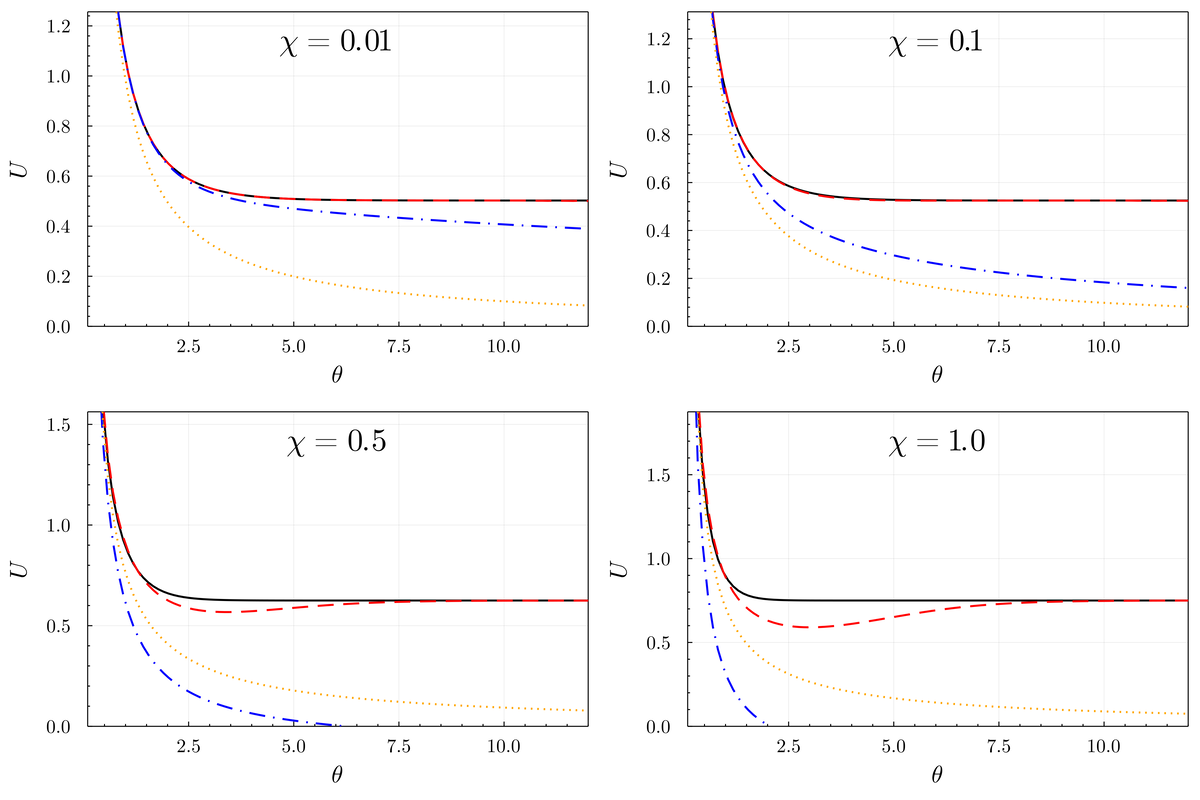
\includegraphics[width=\textwidth]{Imagens/energias_kerr.png}
    \centering
    \caption{Energia como função do tempo térmico para diferentes valores de $\chi$. Linha preta cheia: resultado exato; linha vermelha tracejada: aproximação semiclássica, linha azul tracejada/pontilhada: aproximação metaplética amortecida; linha amarela pontilhada: resultado clássico.}
    \label{energias kerr}
\end{figure}

Para avaliar como a qualidade da aproximação depende de $\chi$, calculamos também o erro percentual relativo entre um resultado aproximado $U_{ap}$ e o resultado exato $U_{ex}$, que definimos como
\begin{equation}
    e\left( U_{ap}, U_{ex} \right) = \left| 1- \frac{ U_{ap}}{U_{ex}} \right| \times 100.
\end{equation}
Os resultados são mostrados na figura \ref{erros relativos kerr}.

\begin{figure}[H]
     \centering
     \begin{subfigure}[b]{0.32\textwidth}
         \centering
         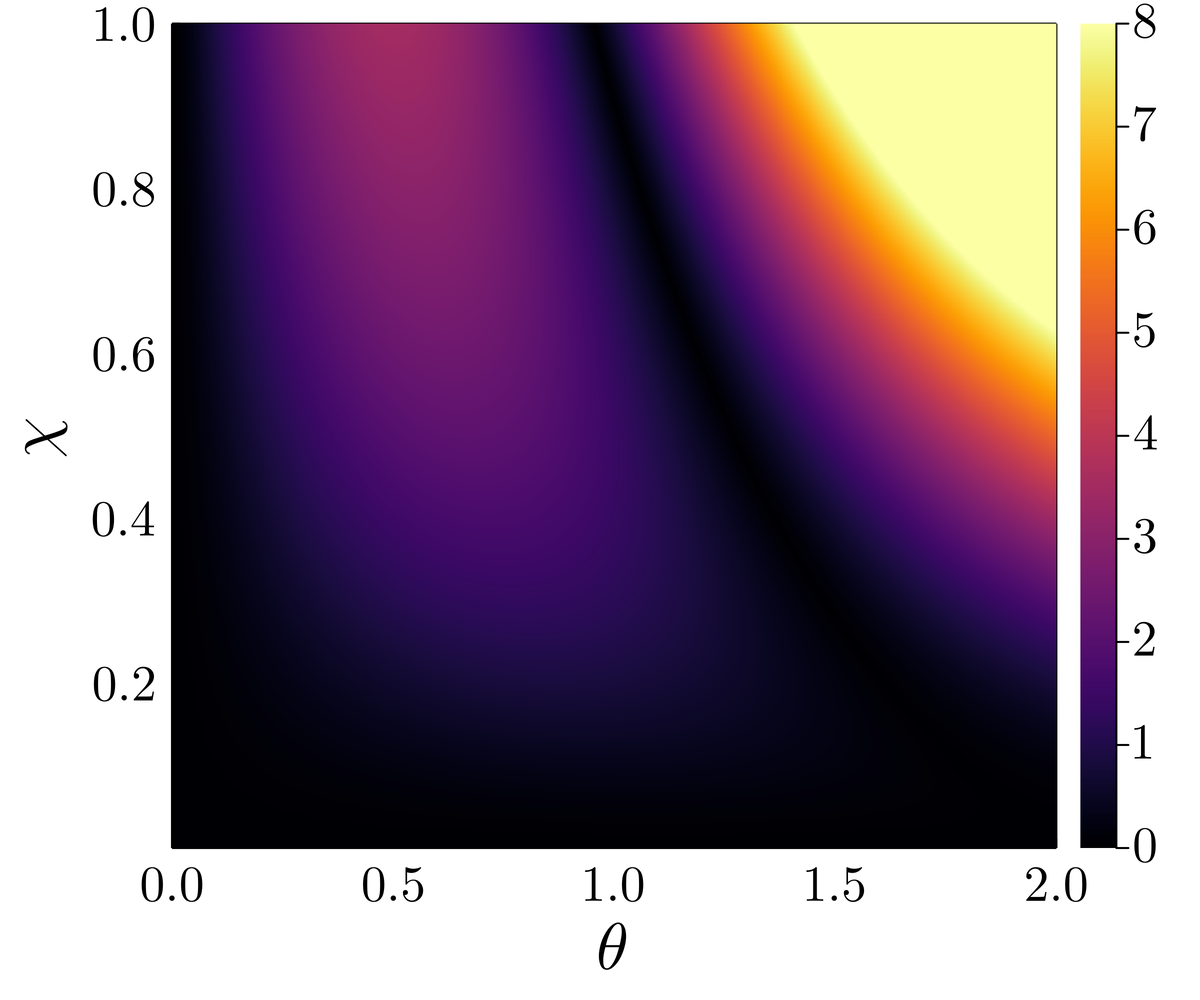
\includegraphics[width=\textwidth]{Imagens/erro_relativo_energia_sc.png}
         \caption{Semiclássica}
         \label{erro relativo kerr sc}
     \end{subfigure}
     \hfill
     \begin{subfigure}[b]{0.32\textwidth}
         \centering
         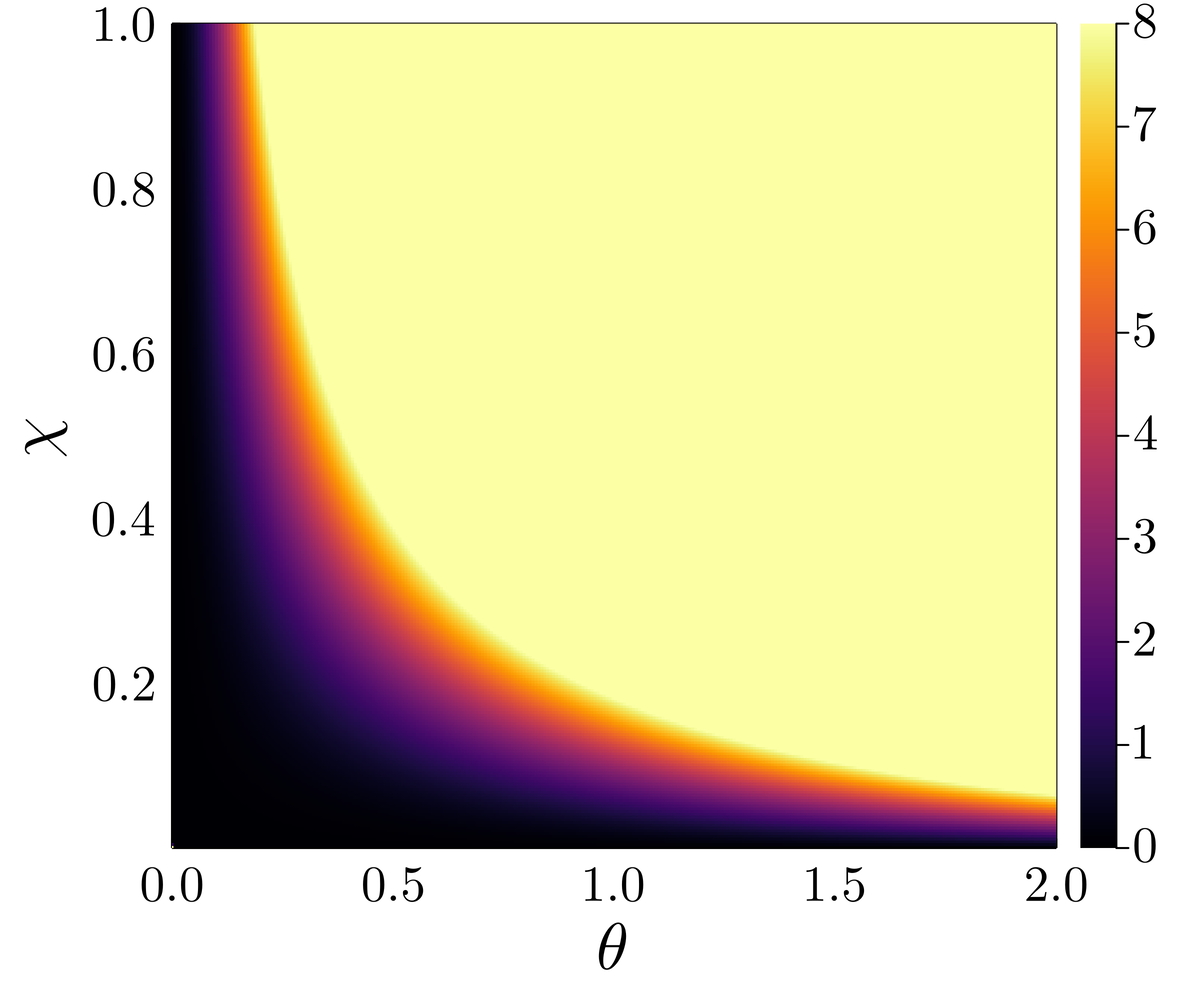
\includegraphics[width=\textwidth]{Imagens/erro_relativo_energia_kerr_dm.png}
         \caption{Metaplética Amortecida}
         \label{fig:three sin x}
     \end{subfigure}
     \hfill
     \begin{subfigure}[b]{0.32\textwidth}
         \centering
         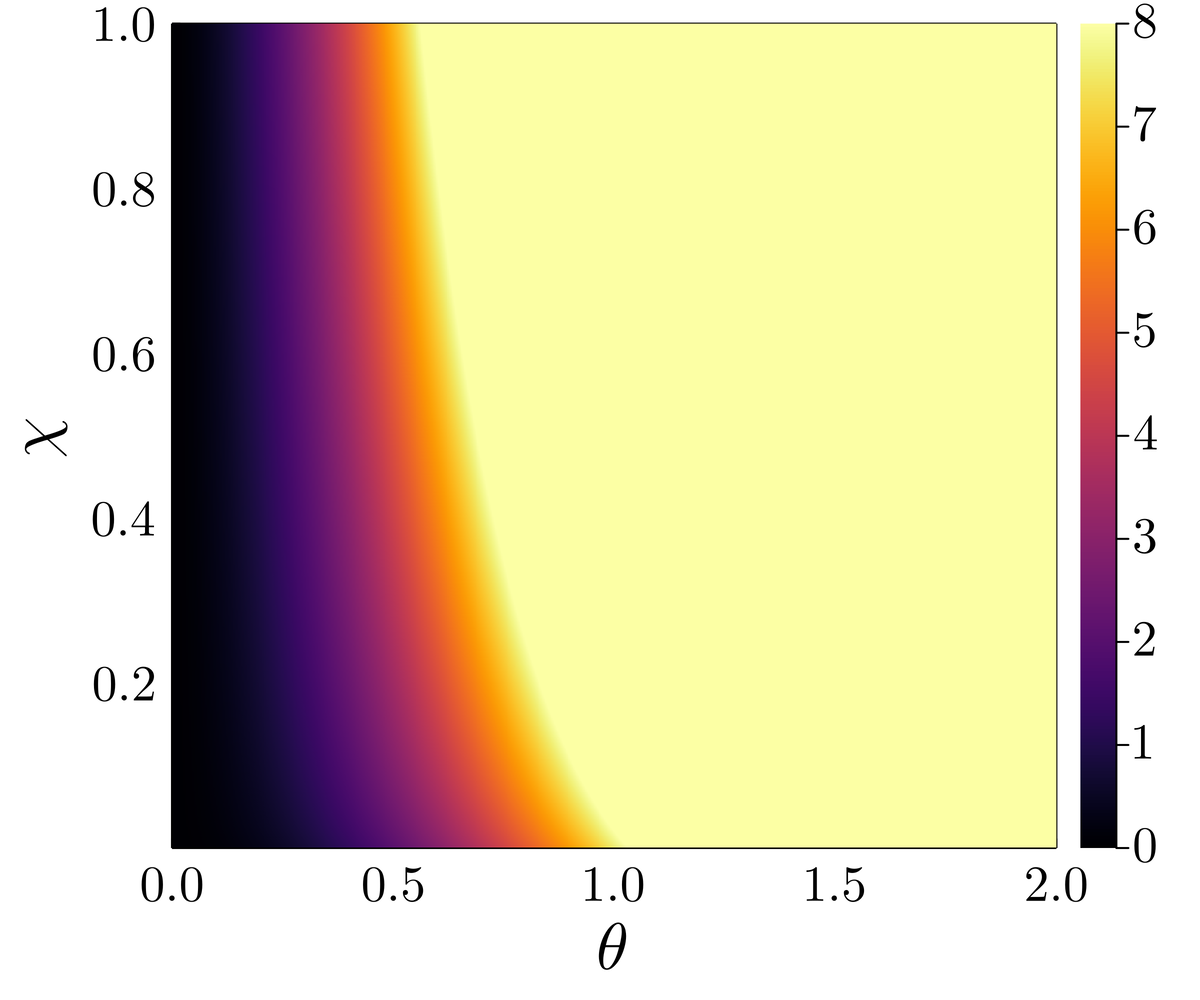
\includegraphics[width=\textwidth]{Imagens/erro_relativo_energia_cl.png}
         \caption{Clássica}
         \label{fig:five over x}
     \end{subfigure}
        \caption{Erros percentuais relativos ao resultado exato como função de $\theta$ e $\chi$.}
        \label{erros relativos kerr}
\end{figure}

Na figura \ref{erro relativo kerr extendido} repetimos a figura \ref{erro relativo kerr sc}, mas com $\theta$ variando sobre um intervalo maior.

\begin{figure}[H]
    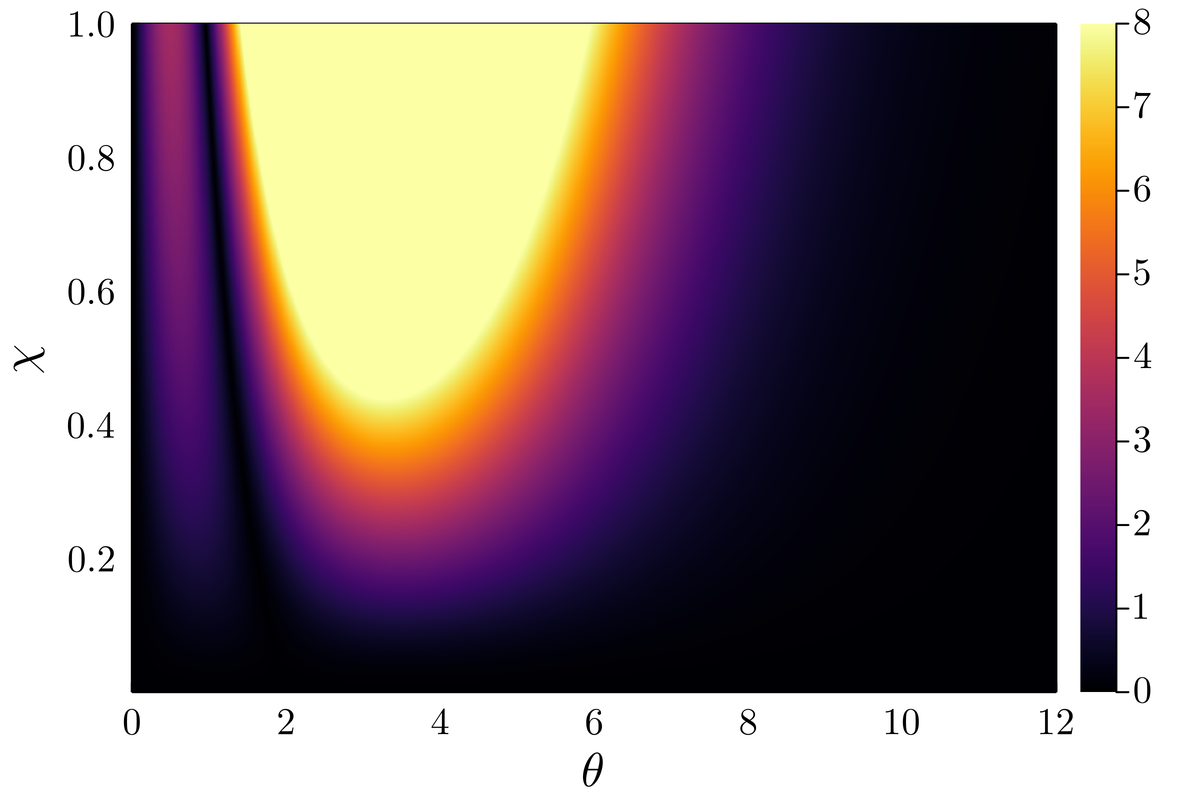
\includegraphics[width=.8\textwidth]{Imagens/erro_relativo_energia_sc_extendido.png}
    \centering
    \caption{Erro percentual da aproximação semiclássica relativo ao resultado exato}
    \label{erro relativo kerr extendido}
\end{figure}

Este gráfico confirma as nossas expectativas de que aproximação semiclássica está bem ancorada em baixas e em altas temperaturas, e também para $\chi \ll 1$. Vemos também que a qualidade de ambas aproximações semiclássicas piora quando $\chi$ cresce, ou seja, quando nos afastamos do regime do oscilador harmônico, e que a aproximação semiclássica completa, em termos de precisão, é claramente superior à metaplética amortecida.

\subsection{Calor Específico}

Vemos que para o cálculo do valor específico através de \eqref{calor específico flutuação}, precisaremos do símbolo de Wigner de $\hat{H}^2$, que é um polinômio em $\left( \hat{p}^2+\hat{q}^2\right)$ de quarta ordem. Os símbolos de Wigner necessários para esse cálculo são encontrados no apêndice \ref{Símbolo de Wigner para formas normais}.

É possível ver que as aproximações semiclássicas não respeitam a propriedade fundamental de que $c>0$, que, do ponto de vista termodinâmico, é uma manifestação da estabilidade do sistema frente as flutuações de energia \cite{callen1991thermodynamics}. Isso já poderia ser antecipado ao notar que o gráfico de energia em função da $\theta$ (figura \ref{energias kerr}) para a aproximação semiclássica completa troca de concavidade. Para $\chi = 0.1$, é possível ver que a aproximação semiclássica erra por baixo, mas, em seguida, tende a $0$, acompanhando o resultado exato. Não é possível ver o mesmo comportamento para $\chi=0.5$ e $\chi = 1$, embora suspeitemos que bastaria continuar a solução por um tempo térmico maior, o que não foi possível devido a instabilidades numéricas. Esse erro significativo para $\theta \gg 1$ pode ser decorrente de um pequeno erro nas flutuações $\expval{\hat{H}^2}_\beta - \expval{\hat{H}}_\beta^2$, mas que é amplificado enormemente ao ser multiplicado por $\beta^2$, como em \eqref{calor específico flutuação}.

\begin{figure}[H]
    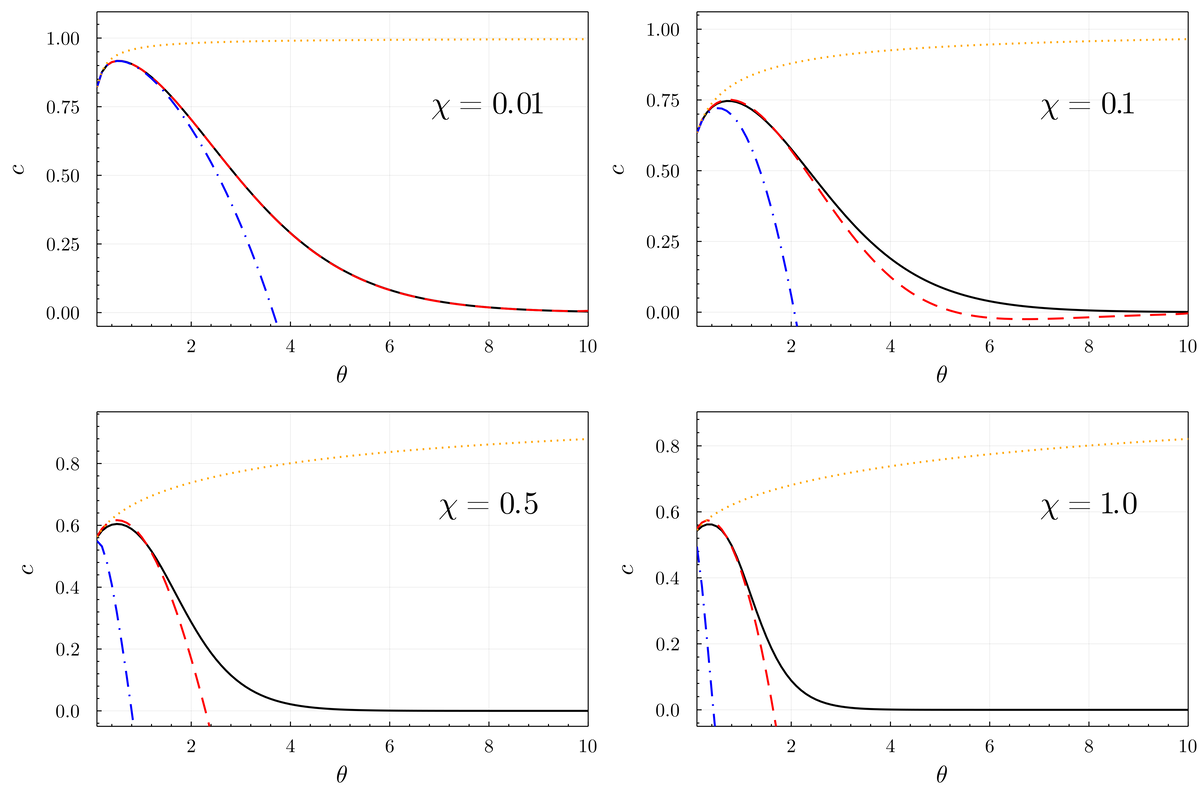
\includegraphics[width=\textwidth]{Imagens/calores_especificos_kerr.png}
    \centering
    \caption{Calor específico como função do tempo térmico para diferentes valores de $\chi$. Linha preta cheia: resultado exato; linha vermelha tracejada: aproximação semiclássica, linha azul tracejada/pontilhada: aproximação metaplética amortecida; linha amarela pontilhada: resultado clássico.}
    \label{calores específicos kerr}
\end{figure}

\begin{figure}[H]
     \centering
     \begin{subfigure}[b]{0.32\textwidth}
         \centering
         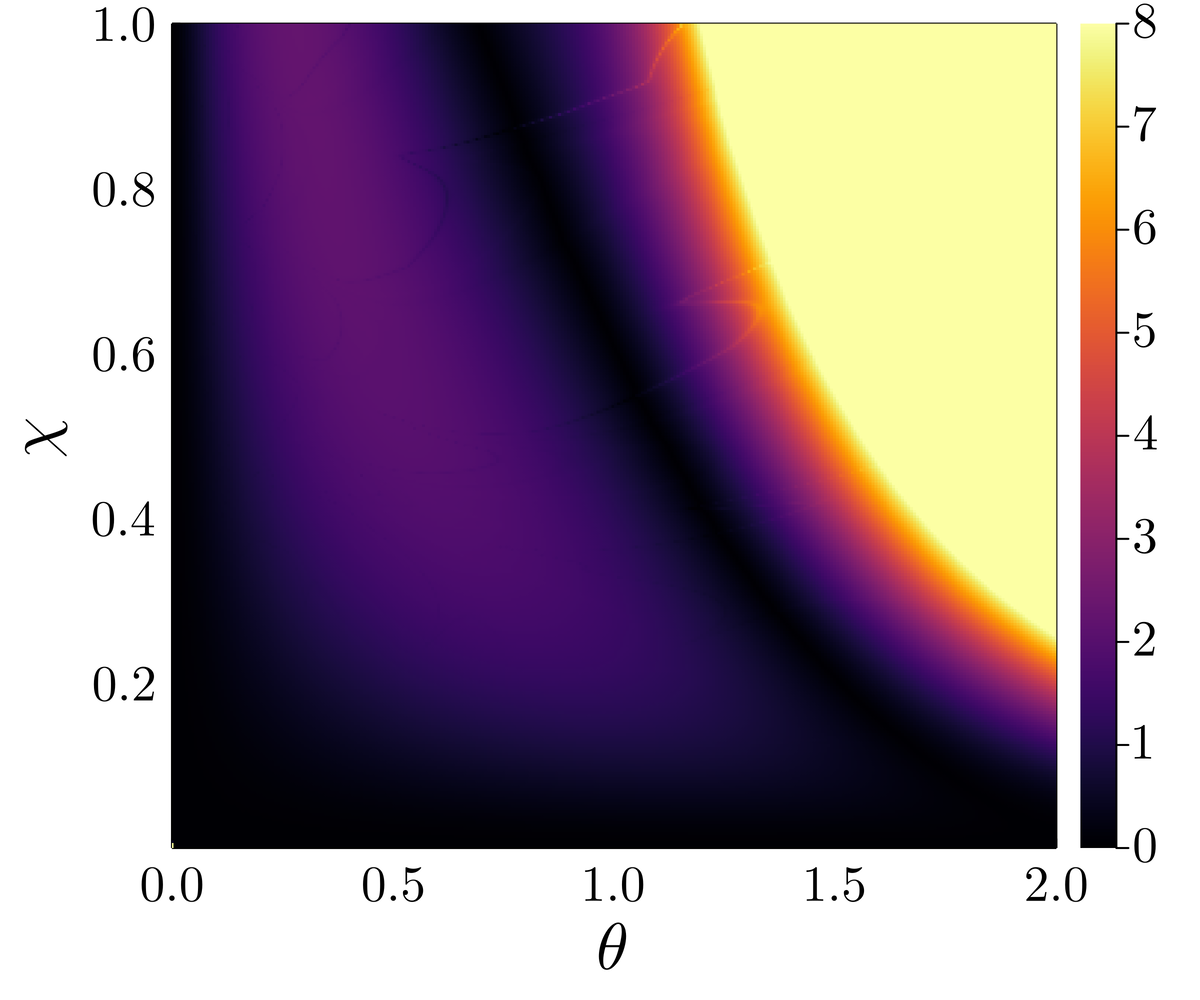
\includegraphics[width=\textwidth]{Imagens/erro_relativo_calor_kerr_sc.png}
         \caption{Semiclássica}
         \label{erro relativo calor kerr sc}
     \end{subfigure}
     \hfill
     \begin{subfigure}[b]{0.32\textwidth}
         \centering
         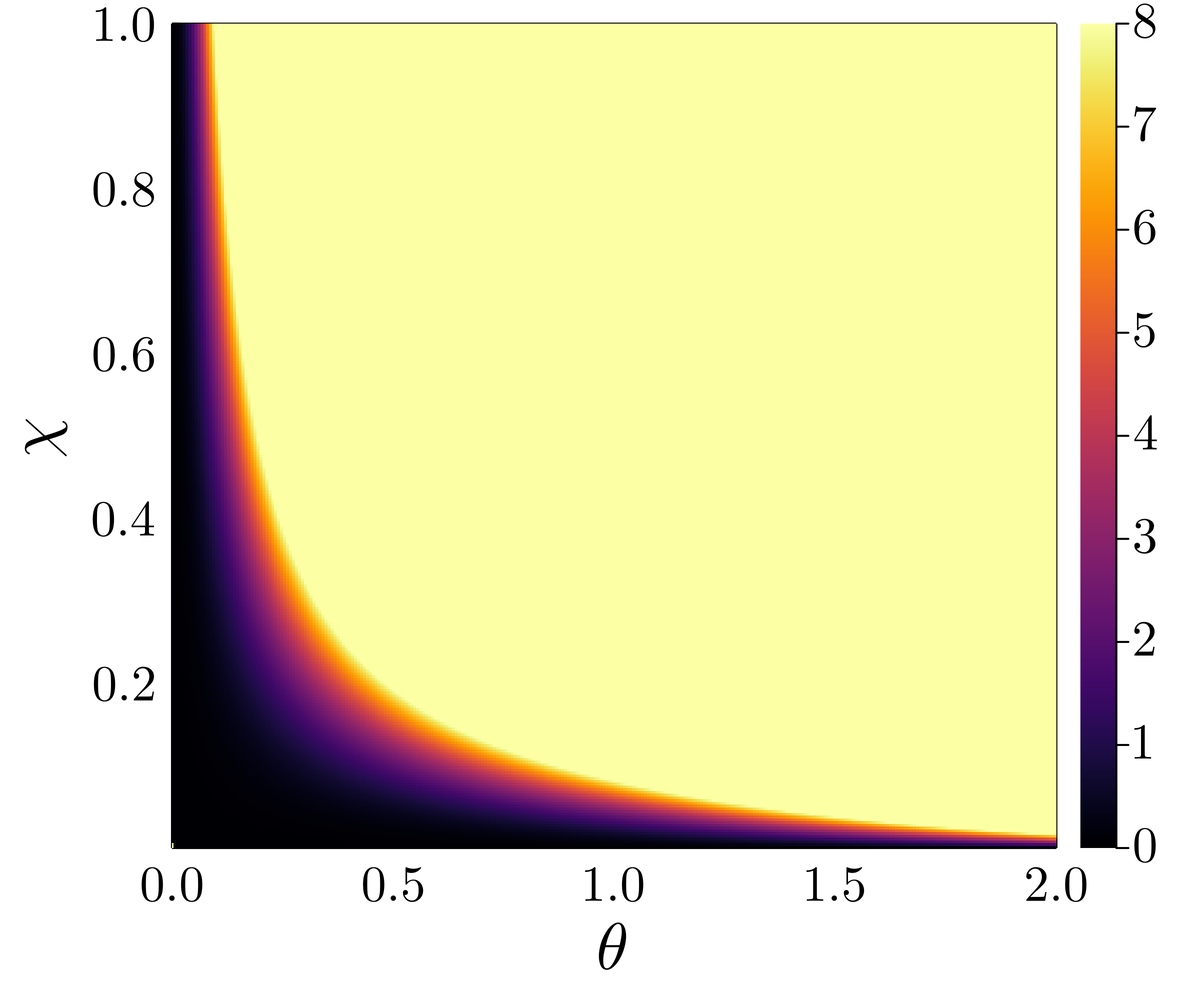
\includegraphics[width=\textwidth]{Imagens/erro_relativo_calor_kerr_dm.png}
         \caption{Metaplética Amortecida}
         \label{erro relativo calor kerr dm}
     \end{subfigure}
     \hfill
     \begin{subfigure}[b]{0.32\textwidth}
         \centering
         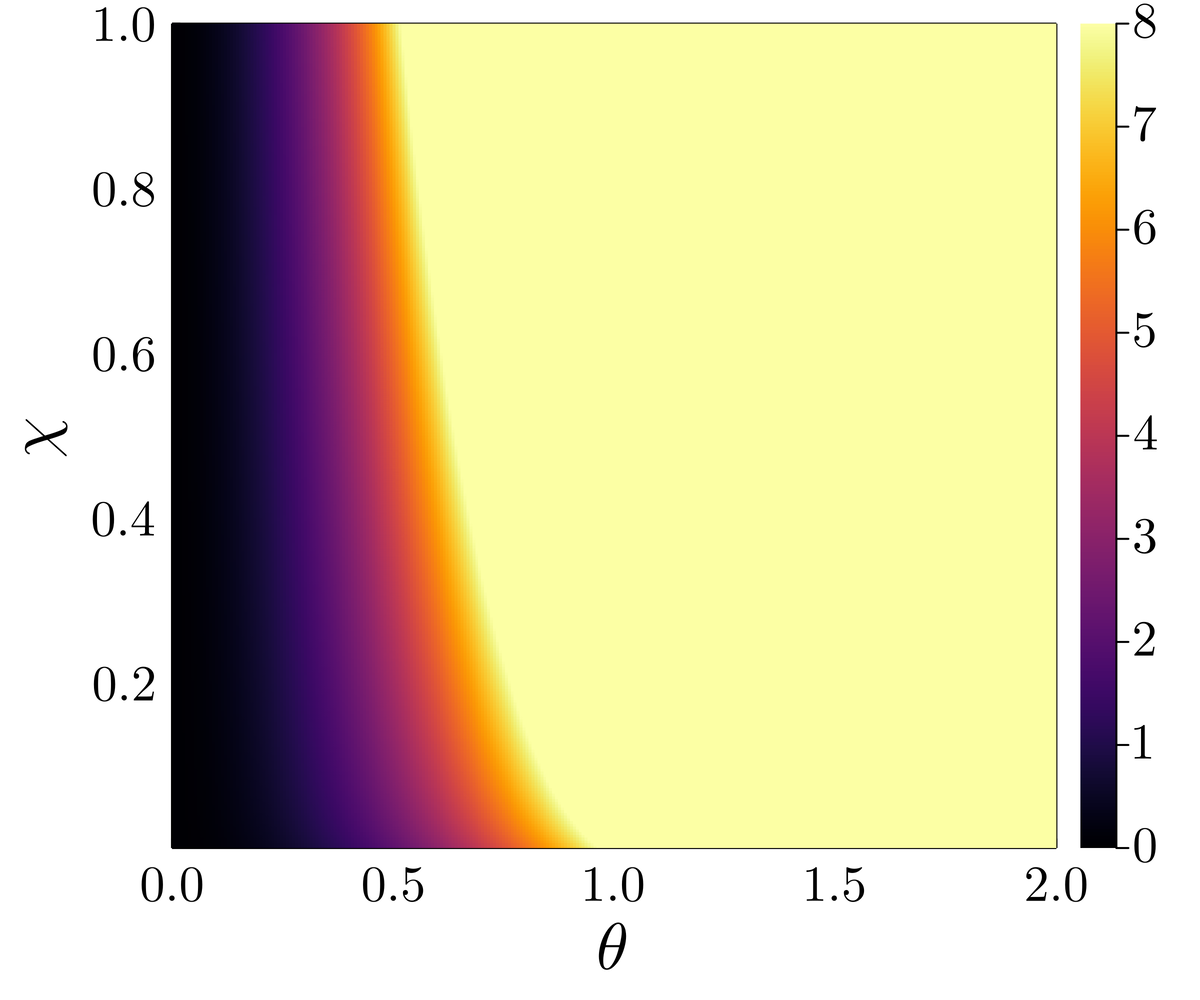
\includegraphics[width=\textwidth]{Imagens/erro_relativo_calor_kerr_cl.png}
         \caption{Clássica}
         \label{erro relativo calor kerr cl}
     \end{subfigure}
        \caption{Erros percentuais relativos ao resultado exato como função de $\theta$ e $\chi$.}
        \label{erros relativos calor kerr}
\end{figure}

De modo qualitativo, o resultado é então o mesmo que aquele observado para a energia, com a exceção de uma discrepância bem maior na região de baixas temperaturas.


\chapter{Aproximação semiclássica para hamiltonianas padrão}
\label{Aproximação semiclássica para hamiltonianas padrão}

Nesse capítulo, discutiremos em detalhe as aproximações semiclássicas para hamiltonianas na forma padrão
\begin{equation}
\label{hamiltoniana padrão}
    \hat{H} = \frac{\hat{p}^2}{2m} + V\left( \hat{q} \right),
\end{equation}
que são de extrema importância. Em seguida, as aplicaremos para o chamado sistema de Morse.

\section{Energia de dissociação}

Para potenciais que satisfazem $\lim_{|q| \to \infty} V(q) = \infty$, o sistema, seja ele clássico ou quântico, apresenta apenas estados ligados. Entretanto, diversos sistemas de interesse, como o elétron de um átomo de hidrogênio, por exemplo, tornam-se livres uma vez que lhe é fornecida uma quantidade suficiente de energia. Para levar em consideração esse efeito, é necessário então utilizar um potencial que é limitado no infinito.

No contexto clássico, um estado corresponde a um ponto no espaço de fase, e podemos definir um estado ligado como um ponto cuja órbita permanece no interior de um conjunto compacto. Todos os estados de sistemas na forma normal de Birkhoff, por exemplo, são ligados, uma vez que, como já discutido, as órbitas são círculos. Por outro lado, para uma partícula livre, de acordo com essa definição, os estados com $p=0$ são ligados, enquanto os demais são livres. Para hamiltonianas
\begin{equation}
    H(p,q) = \frac{p^2}{2m} + V\left( q \right),
\end{equation}
podemos definir uma energia de dissociação $D$ como
\begin{equation}
\label{energia de dissociação}
    D = \min \left\{ \lim_{q \to \infty} V(q), \lim_{q \to -\infty} V(q) \right\}
\end{equation}
Desta forma, estados com $H(p,q) < D$ são ligados, enquanto estados com $H(p,q) > D$ são livres. Notamos que, tipicamente no caso de ser uma coordenada radial, $q$ não pode assumir valores em todo $\mathbb{R}$, de forma que, em \eqref{energia de dissociação} deve-se considerar apenas o limite que fizer sentido.

No contexto da mecânica estatística, essa discussão é importante pois, frequentemente, estamos interessados apenas em regimes de temperatura nos quais $kT \ll D$. Por exemplo, podemos querer analisar um gás molecular a temperaturas baixas o suficientes para que o efeito da dissociação das moléculas seja desprezível. A prescrição clássica para o cálculo de quantidades termodinâmicas nesse contexto é a realização das integrais relevantes apenas sobre a região $R$ correspondente aos estados ligados \cite{riganelli2001rovibrational}. A função de partição, por exemplo, seria dada então por
\begin{equation}
\label{função de partição classica estados ligados}
    Z_{cl} = \int_R \frac{dp dq}{2\pi \hbar} e^{-\beta H(p,q)}.
\end{equation}
Notamos que, para sistemas que não satisfazem $\lim_{|q| \to \infty} V(q) = \infty$, as integrais da forma \eqref{função de partição classica estados ligados} não convergem quando integradas sobre todo o espaço de fase, uma vez que o integrando não tende a $0$ quando $|q| \to \infty$.

Já no contexto quântico, a situação é mais direta — no regime $kT \ll D$, consideramos apenas o conjunto discreto $\{ \ket{n} , \ n=0,\ldots,N\}, \ N \le \infty,$ de estados ligados cuja probabilidade de ocupação é
\begin{equation}
    p_j = \frac{e^{-\beta E_j}}{Z_\beta}, \ \ \ Z_\beta = \sum_{n=0}^{N} e^{-\beta E_j},
\end{equation}
de forma que o operador densidade é
\begin{equation}
    \hat{\rho} = \frac{1}{Z_\beta}\sum_{n=0}^{N} e^{-\beta E_j} \ket{n} \bra{n}
\end{equation}
e a função de Wigner é
\begin{equation}
    W_\beta(\mathbf{x}) = \sum_{n=0}^{N} p_j W_n(\mathbf{x}) .
\end{equation}
O problema para a aplicação de nossas aproximações semiclássicas é que, agora, os estados ligados não formam mais uma base para o espaço de Hilbert. A relação de completeza
\begin{equation}
    \hat{I} = \sum_{n=0}^{N} \ket{n} \bra{n} + \int d \lambda D(\lambda) \ket{\lambda} \bra{\lambda}
\end{equation}
também inclui autoestados livres $\ket{\lambda}$, correspondentes a autoenergias $E_\lambda$, sendo $\lambda$ um parâmetro contínuo e $D(\lambda)$ uma densidade de estados. Desta forma, o propagador agora é escrito como
\begin{equation}
    \hat{U}_t = e^{-it \hat{H}/\hbar} = \sum_{n=0}^{N} e^{-it E_j/\hbar} \ket{n} \bra{n} + \int d \lambda D(\lambda) e^{-it E_\lambda/\hbar} \ket{\lambda} \bra{\lambda} 
\end{equation}
de forma que sua continuação analítica
\begin{equation}
    \hat{U}_{-i\theta} = e^{-\beta \hat{H}} = \sum_{n=0}^{N} e^{-\beta E_j} \ket{n} \bra{n} + \int d \lambda D(\lambda)  e^{-\beta E_\lambda } \ket{\lambda} \bra{\lambda}
\end{equation}
também contém termos correspondentes aos autoestados livres.

Para remediar essa situação, observamos que as funções de Wigner de autoestados de um operador hamiltoniano apresentam ecos da estrutura das curvas de nível da hamiltoniana clássica. Na figura \ref{autoestados oscilador}, por exemplo, ilustramos as funções de Wigner de alguns autoestados do oscilador harmônico superpostas à curva de nível da autoenergia correspondente. Podemos observar que a função de Wigner se concentra na região com $H(p,q)<E_n$. Tendo isso em vista, seria plausível concluir que, se $\mathbf{x} \notin R$ a maior parte da contribuição para $\hat{U}_{-i\theta}(\mathbf{x})$ vem dos termos correspondentes ao espectro contínuo e, uma maneira efetiva de filtrar essa contribuição seria então efetuar as integrais utilizadas na aproximação semiclássica apenas na região $\mathbf{x} \in R$, exatamente como a prescrição clássica \eqref{função de partição classica estados ligados}. 

\begin{figure}[H]
    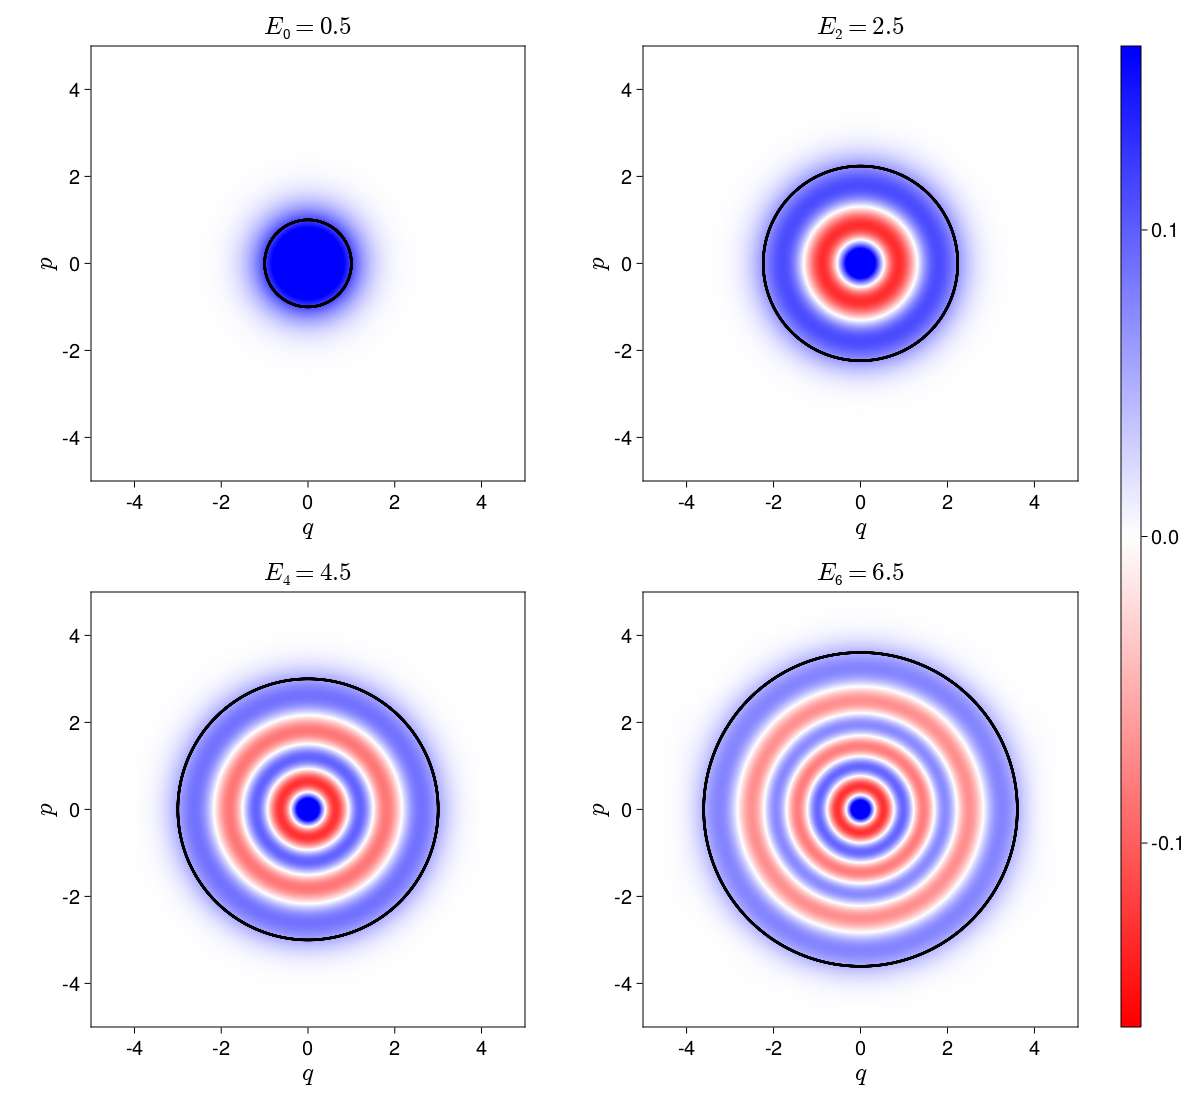
\includegraphics[width=\textwidth]{Imagens/wigner_harmonic_oscilator.png}
    \centering
    \caption{Funções de Wigner para os quatro primeiros autoestados do oscilador harmônico. O círculo preto corresponde aos pontos que satisfazem $H(p,q) = E_n$.}
    \label{autoestados oscilador}
\end{figure}

Entretanto, por si só, esse exemplo é enganoso, e devemos tomar um pouco de cuidado. Para ver isso, considere um sistema formado por uma partícula de massa $m$ se movendo sob a ação de um potencial do tipo poço duplo, dado pela expressão
\begin{equation}
    V(x) = V_0 \left[ \left( \frac{x}{l}\right)^4 - 2\left( \frac{x}{l}\right)^2\right],
\end{equation}
sendo $l$ um comprimento e $V_0$ a profundidade do poço, como na figura \ref{potencial poço duplo}. 

\begin{figure}[H]
    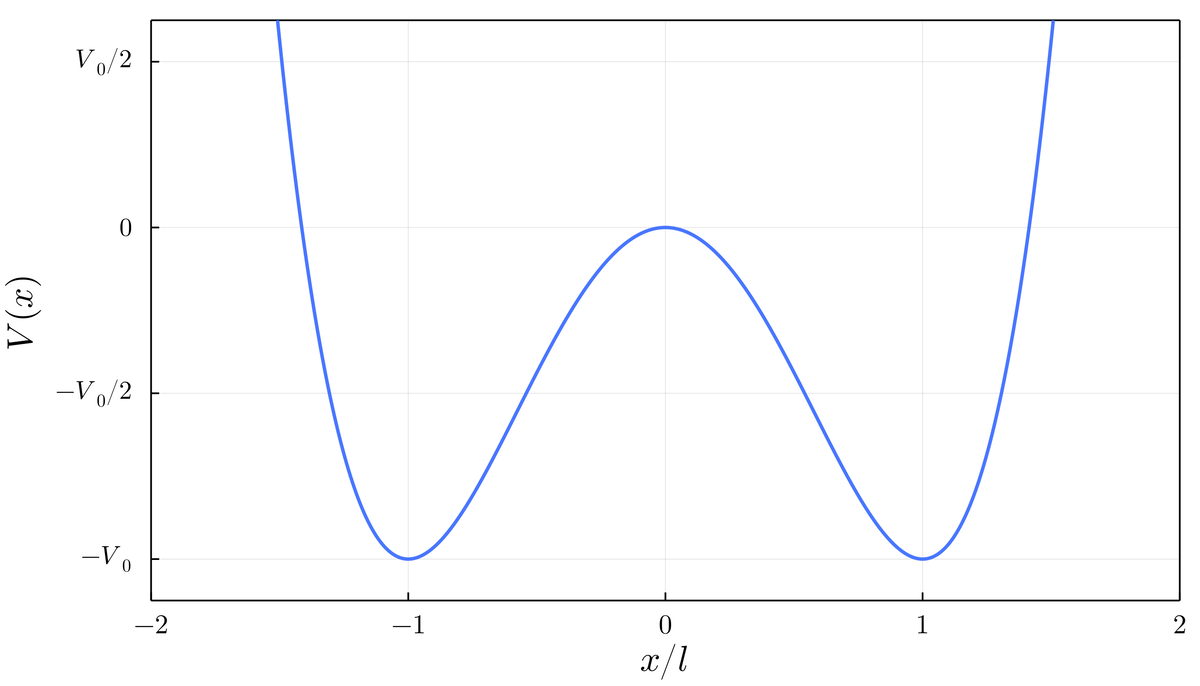
\includegraphics[width=.7\textwidth]{Imagens/double_well_potential.png}
    \centering
    \caption{Potencial poço duplo.}
    \label{potencial poço duplo}
\end{figure}

Introduzindo a coordenada adimensional $q = x/l$, a frequência $\omega = \sqrt{2V_0/ml^2}$ e a constante $v_0 = 2V_0/\hbar \omega$, podemos escrever a hamiltoniana desse sistema como
\begin{equation}
    H(p,q) = \frac{\hbar \omega}{2} \left[ \frac{1}{v_0} \left( \frac{p}{\hbar}\right)^2 + v_0\left( q^4-2q^2\right) \right],
\end{equation}
sendo $p$ o momento canonicamente conjugado a $q$. Vemos que se $E < 0$ então a curva de nível é formada por duas partes desconexas e a discussão anterior nos levaria então a supor que a função de Wigner se concentra apenas no interior dessas duas partes. Entretanto, como pode ser visto na figura \ref{autoestados poço duplo}, isso não é verdade.

De acordo com a determinação semiclássica das funções de Wigner para autoestados feita em \cite{berry1977semi}, a função de Wigner próxima a um ponto $(p,q)$ será significativamente não nula apenas se for possível encontrar uma corda centrada em $(p,q)$ cujas extremidades estão na curva de nível de energia. Vemos então que, para curvas de níveis que delimitam regiões convexas, como o caso do oscilador harmônico, podemos afirmar de fato que a função de Wigner se concentra no interior da curva de nível. Por outro lado, no caso extremo de uma curva de nível disjunta, como no poço duplo, seriamos levados a erros significativos ao nos restringir a tal região. Entretanto, essa discussão nos permite propor uma simples correção à prescrição clássica, que seria realizar a integração sobre a \textit{envoltória convexa} \footnote{Dado um subconjunto $R$ de um espaço vetorial, a sua envoltória convexa pode ser definida como o conjunto $\mathcal{C}(R) = \left\{ \sum_k t_k v_k \ | \ v_k \in R ; \ \sum_k t_k = 1 \right\}$ formada por todas as combinações convexas dos pontos de $R$ \cite{lima2016algebra}. Em particular, ele contem qualquer segmento de reta com extremidades em $R$.} $\mathcal{C}(R)$ da região classicamente permitida.

\begin{figure}[H]
    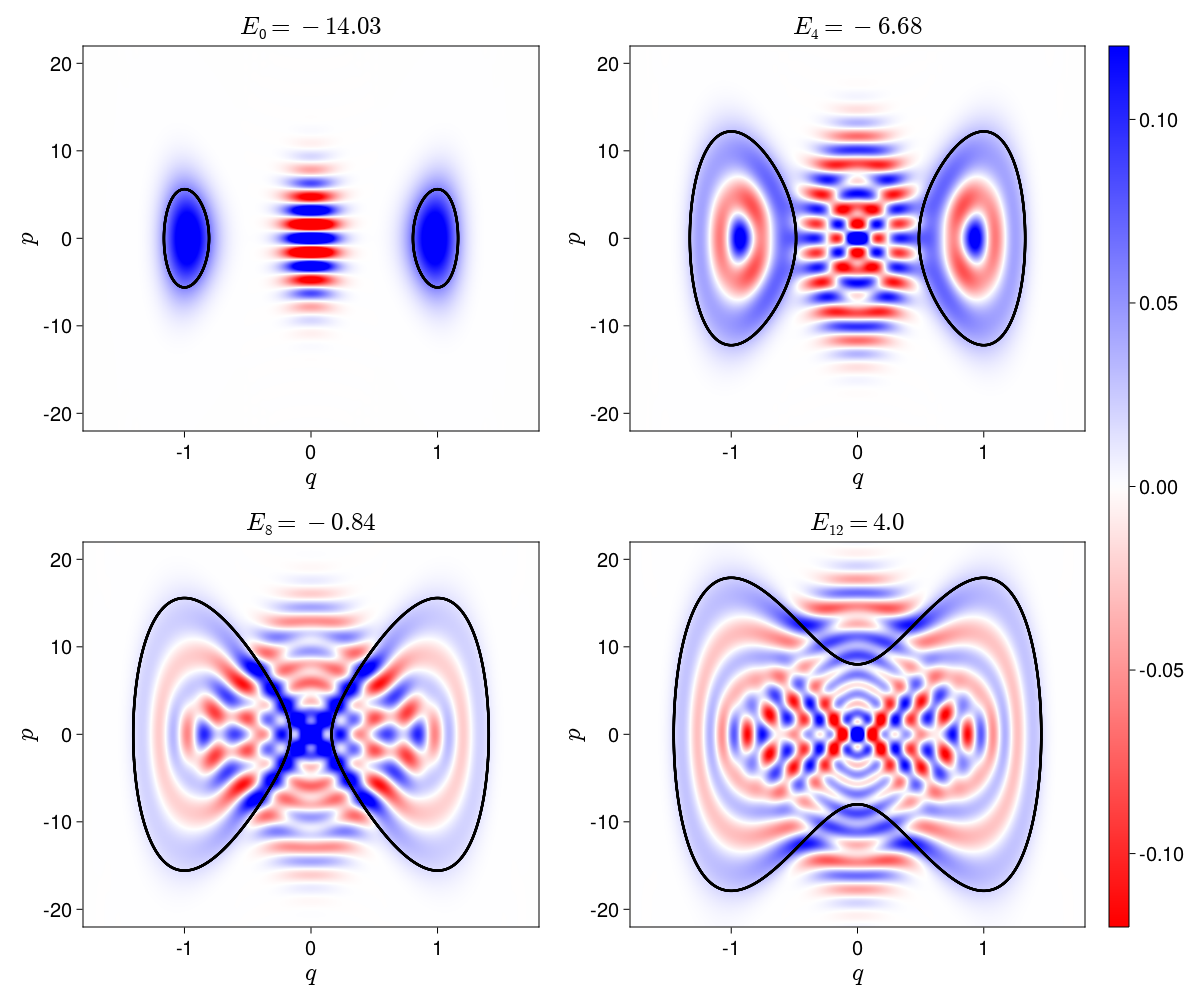
\includegraphics[width=\textwidth]{Imagens/wigner_double_well.png}
    \centering
    \caption{Funções de Wigner para autoestados do poço duplo. A curva preta corresponde aos pontos que satisfazem $H(p,q) = E_n$. Utilizamos unidades nas quais $\hbar = \omega/2 = 1$ e tomamos $v_0 = 16$.}
    \label{autoestados poço duplo}
\end{figure}

Notamos, contudo, que as integrais que estamos utilizando para o cálculo das médias termodinâmicas, como em \eqref{aproximação semiclassica termica}, por exemplo, são expressas em termos do ponto médio da trajetória $\mathbf{X}$, e não do centro $\mathbf{x}$, sendo este último, nesse contexto, uma função de $\mathbf{X}$ e $\mathbf{\theta}$: $\mathbf{x} = F_\theta (\mathbf{X})$. Se fossemos seguir esta prescrição com rigor, teríamos então que realizar as integrais sob a condição $\mathbf{X} \in F_\theta^{-1} (\mathcal{C}(R))$, e então, para cada $\theta$, seria necessário atualizar a região de integração, que, possivelmente, evoluiria de forma complicada. Felizmente, pelo menos no caso que estudaremos, o sistema de Morse, as curvas de nível dos estados menos excitados são aproximadamente convexas, isto é $\mathcal{C}(R) \approx R$, e realizar a integração sob a condição mais simples $\mathbf{X} \in R$ foi suficiente para obter excelentes resultados.

\section{Aproximações semiclássicas para hamiltonianas na forma padrão}

Nessa seção, discutimos algumas fórmulas genéricas para hamiltonianas na forma padrão $H = p^2/2m + V(q)$ que facilitam a aplicação das aproximações semiclássicas.

\subsection{Aproximação Metaplética Amortecida}

Para hamiltonianas na forma padrão, temos
\begin{equation}
\label{Aproximação Metaplética Amortecida padrão}
    \mathbf{h}_{\mathbf{x}} = \begin{pmatrix} p/m \\ V'(q) \end{pmatrix}; \ \ \ \boldsymbol{\mathcal{H}}_{\mathbf{x}} = \begin{pmatrix} 1/m & 0 \\ 0 & V''(q) \end{pmatrix};  \ \ \ \text{adj } \boldsymbol{\mathcal{H}}_{\mathbf{x}} = \begin{pmatrix} V''(q) & 0  \\ 0 & 1/m \end{pmatrix}; \ \ \ \Omega_\mathbf{x}^2 = \frac{V''(q)}{m},
\end{equation}
de forma que
\begin{equation}
    \begin{aligned}
        \frac{g(\alpha) \theta^2}{8} \left( \text{adj } \boldsymbol{\mathcal{H}}_\mathbf{x} \right) \mathbf{h}_\mathbf{x} \cdot \mathbf{h}_\mathbf{x} &= \frac{g(\alpha) \theta^2}{8m} \left[ \frac{V''(q)}{m}p^2 + V'(q)^2 \right] \\ &= \left[1-f(\alpha)\right] \frac{p^2}{2m} + g(\alpha) \frac{{\left[\theta V'(q) \right]}^2}{8m},
    \end{aligned}
\end{equation}
e, então,
\begin{equation}
    e^{-\beta \hat{H}} \left( \mathbf{x}\right)_{DM} =  \sech \alpha  \exp \left\{ -\beta \left[ \frac{f(\alpha)p^2}{2m} +V(q) - g(\alpha) \frac{{\left[\theta V'(q) \right]}^2}{8m} \right] \right\}.
\end{equation}
Já a região de integração pode ser escrita como
\begin{equation}
    R = \begin{cases}
        q_- \le q \le q_+ \\
        |p| \le \sqrt{2m \tilde{V}(q)}
    \end{cases}
\end{equation}
sendo $\Tilde{V} = D - V(q)$ e $q_{\pm}$ as soluções de $V(q_{\pm}) = D$.

Logo, nessa aproximação, a função de partição para os estados ligados é dada por
\begin{equation}
\label{f partição 111}
    \begin{aligned}
        Z = \frac{1}{2\pi \hbar}\int_{q_-}^{q_+} & dq \ \sech{\alpha} \ e^{-\sigma} \int_{-\sqrt{2m\Tilde{V}}}^{\sqrt{2m\Tilde{V}}} dp \ e^{-\beta f(\alpha)p^2/2m}  
    \end{aligned}
\end{equation}
onde, por brevidade, definimos
\begin{equation}
    \sigma = \beta \left[V(q) - g(\alpha) \frac{{\left[\theta V'(q) \right]}^2}{8m} \right].
\end{equation}

Notamos que a integral em $p$ pode ser expressa em termos da função erro $\erf$:
\begin{equation}
    \frac{1}{2\pi \hbar}\int_{-\sqrt{2m\Tilde{V}}}^{\sqrt{2m\Tilde{V}}} dp \ e^{-\beta fp^2/2m} = \sqrt{\frac{ m}{2\pi \hbar^2 \beta f}} \erf \left( \sqrt{\beta f \Tilde{V}} \right) =  \frac{ 1}{ \lambda_T \sqrt{f}} \erf \left( \sqrt{\beta f \Tilde{V}} \right)
\end{equation}
sendo
\begin{equation}
    \lambda_T = \sqrt{\frac{2\pi \hbar^2}{m k_b T}}
\end{equation}
o comprimento de onda térmico e passamos a abreviar $f = f(\alpha)$. Substituindo essa expressão em \eqref{f partição 111}, chegamos a
\begin{equation}
    \begin{aligned}
        Z = \frac{1}{\lambda_T}\int_{q_-}^{q_+} & dq \ \frac{\sech{\alpha} \  e^{-\sigma}}{\sqrt{f}} \erf \left( \sqrt{\beta f \Tilde{V}} \right).
    \end{aligned}
\end{equation}

Para o cálculo do valor esperado de observáveis, será conveniente obter uma expressão para
\begin{equation}
    I_n = \frac{\lambda_T \sqrt{f}}{2\pi \hbar}\int_{-\sqrt{2m\Tilde{V}}}^{\sqrt{2m\Tilde{V}}} \ \left( \frac{p^2}{2m} \right)^n \ e^{-\beta fp^2/2m} dp.
\end{equation}
Realizando integração por partes, deduz-se à relação de recorrência
\begin{equation}
    \begin{aligned}
        I_{n+1} &= \frac{1}{\beta f} \left[ \left(n + \frac{1}{2} \right)I_{n} - \tilde{V}^n \sqrt{\frac{\beta f \Tilde{V}}{\pi}} e^{-\beta f\Tilde{V}} \right], \ \ \ I_0 = \erf \left( \sqrt{\beta f \Tilde{V}} \right),
    \end{aligned}
\end{equation}
de forma que, introduzindo o operador energia cinética $\hat{K} = \hat{p}^2/2m$, temos
\begin{equation}
    \expval{\hat{K}^n} = \frac{1}{\lambda_T Z}  \int_{q_-}^{q_+}  dq \ \frac{\sech{\alpha} \  e^{-\sigma}}{\sqrt{f}} I_n
\end{equation}

Em particular, temos
\begin{equation}
    \begin{aligned}
        \expval{\hat{K}} = \frac{1}{\lambda_T Z} &  \int_{q_-}^{q_+}  dq \ \frac{\sech{\alpha} \  e^{-\sigma}}{\sqrt{f}} \\ &\times \frac{1}{\beta f  } \left[ \frac{1}{2} \erf \left( \sqrt{\beta f \Tilde{V}} \right) - \sqrt{\frac{\beta f \Tilde{V}}{\pi}} e^{-\beta f\Tilde{V}} \right]
    \end{aligned}
\end{equation}
e, então,
\begin{equation}
    \begin{aligned}
        \expval{\hat{H}} = \frac{1}{\lambda_T Z} &  \int_{q_-}^{q_+}  dq \  \frac{\sech{\alpha} \  e^{-\sigma}}{\sqrt{f}} \\ &\times  \left[ \left( \frac{1}{2\beta f} + V \right) \erf \left( \sqrt{\beta f \Tilde{V}} \right) -\frac{1}{f}\sqrt{\frac{\Tilde{V}}{\pi \beta }} e^{-\beta f\Tilde{V}} \right].
    \end{aligned}
\end{equation}
Quando $D \to \infty$, temos $\tilde{V} \to \infty$, o que simplifica a relação de recorrência:
\begin{equation}
    \begin{aligned}
        I_{n+1} &= \frac{1}{\beta f} \left(n + \frac{1}{2} \right)I_{n}, \ \ \ I_0 = 1.
    \end{aligned}
\end{equation}
Obtemos então
\begin{equation}
    \begin{aligned}
        Z = \frac{1}{\lambda_T}\int_{q_-}^{q_+} & dq \ \frac{\sech{\alpha} \  e^{-\sigma}}{\sqrt{f}}
    \end{aligned}
\end{equation}
e
\begin{equation}
    \begin{aligned}
        \expval{\hat{H}} =  \frac{1}{\lambda_T Z} & \int_{q_-}^{q_+}  dq \ \frac{\sech{\alpha} \  e^{-\sigma}}{\sqrt{f}} \left( \frac{1}{2\beta f} + V \right)
    \end{aligned},
\end{equation}


\subsection{Espaço de Fase Duplo}

Se supormos uma hamiltoniana na forma padrão $H(p,q) = p^2/2m + V(q)$, então a hamiltoniana modificada é
\begin{equation}
    \mathbb{H}(\mathbf{x},\mathbf{y}) = \frac{1}{m}\left(p^2-\frac{y_q^2}{4}\right) + \mathbb{V}(q,y_p),
\end{equation}
onde definimos o potencial modificado $\mathbb{V}$ por
\begin{equation}
\label{potencial duplo}
    \mathbb{V}(q,y_p) = V\left(q + \frac{i}{2}y_p\right) + V\left(q - \frac{i}{2}y_p\right)
\end{equation}
e, nesse caso, as equações de movimento ficam
\begin{align*}
    \frac{d y_p}{d \theta} &= - \frac{2p}{m} \Label{aa}&  \frac{d y_q}{d \theta} &= - \frac{\partial \mathbb{V}}{\partial q} \Label{b}\\
    \frac{d p}{d \theta}  &=  \frac{\partial \mathbb{V}}{\partial y_p} \Label{c} & \frac{d q}{d \theta} &= - \frac{y_q}{2m} \Label{d}
\end{align*}

\section{O sistema de Morse}

Com o objetivo de aplicar o formalismo desenvolvido a um sistema concreto, focaremos nossa atenção no potencial de Morse \cite{morse1929diatomic}, ilustrado na Figura \ref{plot potencial morse}, cuja expressão é
\begin{equation}
    V(r) = D \left[ 1-e^{-a(r-r_e)} \right]^2,
\end{equation}
sendo $r$ a coordenada radial, $D$ a energia de dissociação, $r_e$ uma distância de equilíbrio e $a$ uma constante com dimensões de inverso de distância. Este potencial modela a vibração de moléculas diatômicas, levando em consideração a possibilidade de dissociação da ligação.

\begin{figure}[H]
    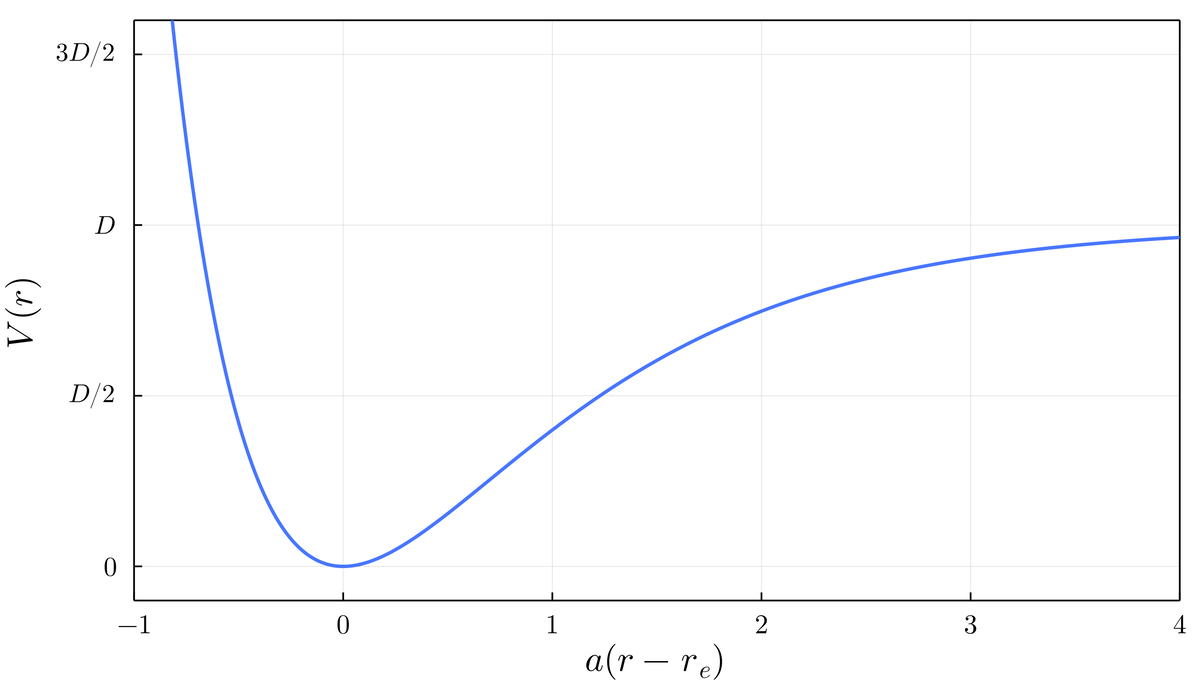
\includegraphics[width=.8\textwidth]{Imagens/plot_morse.png}
    \centering
    \caption{Potencial de Morse}
    \label{plot potencial morse}
\end{figure}

Para diminuir a quantidade de parâmetros livres, é conveniente definir a coordenada adimensional $q = a(r-r_e)$ e a frequência
\begin{equation}
    \omega = \sqrt{\frac{2Da^2}{m}}.
\end{equation}
Desta forma, temos $\dot{q} = a \dot{r}$ e a lagrangiana fica
\begin{equation}
    L = \frac{m \dot{r}^2}{2} - V(r) = D \left[ \left( \frac{\dot{q}}{\omega} \right)^2 - \left( 1-e^{-q} \right)^2 \right],
\end{equation}
a partir da qual obtemos um momento conjugado
\begin{equation}
    p = \frac{\partial L}{\partial \dot{q}} = \frac{2D\dot{q}}{\omega^2}
\end{equation}
e uma hamiltoniana
\begin{equation}
    H = p \dot{q} - L = \frac{\omega^2p^2}{4D} + D\left(1-e^{-q}\right)^2.
\end{equation}
Também é útil definir o parâmetro adimensional
\begin{equation}
    \chi = \frac{\hbar \omega}{4D},
\end{equation}
o que nos permite reescrever $H$ como
\begin{equation}
    H(p,q) = \hbar \omega \left[ \chi \left( \frac{p}{\hbar} \right)^2 + \frac{1}{4\chi}\left( 1-e^{-q} \right)^2 \right].
\end{equation}

A quantização desta hamiltoniana gera um operador com uma quantidade finita de estados ligados, cujas energias são dadas por
\begin{equation}
    E_n = \hbar \omega \left[ \left( n + \frac{1}{2} \right) - \chi \left( n + \frac{1}{2} \right)^2 \right], \ \ \ n = 0,1, \ldots, N
\end{equation}
sendo
\begin{equation}
\label{numero de estados ligados}
    N=\left \lfloor{\frac{1}{2\chi} - \frac{1}{2}}\right \rfloor, 
\end{equation}
onde $\left \lfloor{x}\right \rfloor $ denota o maior inteiro menor que $x$. Para que tenhamos uma ideia da ordem de grandeza em casos fisicamente relevantes, exibimos, na Tabela \ref{dados moleculares}, os valores de $\chi$ e $N$ que melhor se adéquam aos resultados experimentais para as moléculas de hidrogênio, oxigênio e nitrogênio.

\begin{table}[H]
    \centering
    \begin{tabular}{ |c|c|c|  }
  \hline
 Molécula  & $\chi$ & $N$ \\
 \hline
 \hline
 $H_2$   & $2.76 \times 10^{-2}$ & $17$\\
 \hline
 $O_2$&   $7.58 \times 10^{-3}$  & $65$  \\
 \hline
 $N_2$ & $6.07 \times 10^{-3}$  & $81$\\
 \hline
\end{tabular}
    \caption{Valores de $\chi$ e $N$ para algumas moléculas. Calculados a partir de \cite{haynes2016crc}.}
    \label{dados moleculares}
\end{table}
Expressões analíticas para as autofunções de onda na representação de posição e momento, bem como para as funções de Wigner correspondentes, podem ser encontradas em \cite{dahl1988morse}. Na figura \ref{wigner morse}, mostramos algumas dessas funções de Wigner, sendo utilizado o valor de $\chi = 0.07$, o que corresponde a $N=6$. Todos os resultados numéricos daqui em diante são feitos em unidades tais que $\hbar = \omega = 1$. A linha preta corresponde aos pontos do espaço de fase que satisfazem $H(p,q) = E_n$. É possível observar que, o último estado ligado tem uma função de Wigner que se estende além da da curva de nível, o que, como já mencionado, pode ser entendido ao notar que esta região não é convexa.

O sistema de Morse é um bom benchmark para as nossas aproximações semiclássicas pois, uma vez fixado o parâmetro $\chi$, a função de partição vibracional exata
\begin{equation}
    Z = \sum_{n=0}^{N} e^{-\beta E_n} = \sum_{n=0}^{N} \exp\left\{ \theta  \omega \left[  \chi \left( n + \frac{1}{2} \right)^2 - \left( n + \frac{1}{2} \right)  \right]  \right\}
\end{equation}
é calculada como uma simples soma, e dela derivam-se todas as quantidades termodinâmicas.

\begin{figure}[H]
    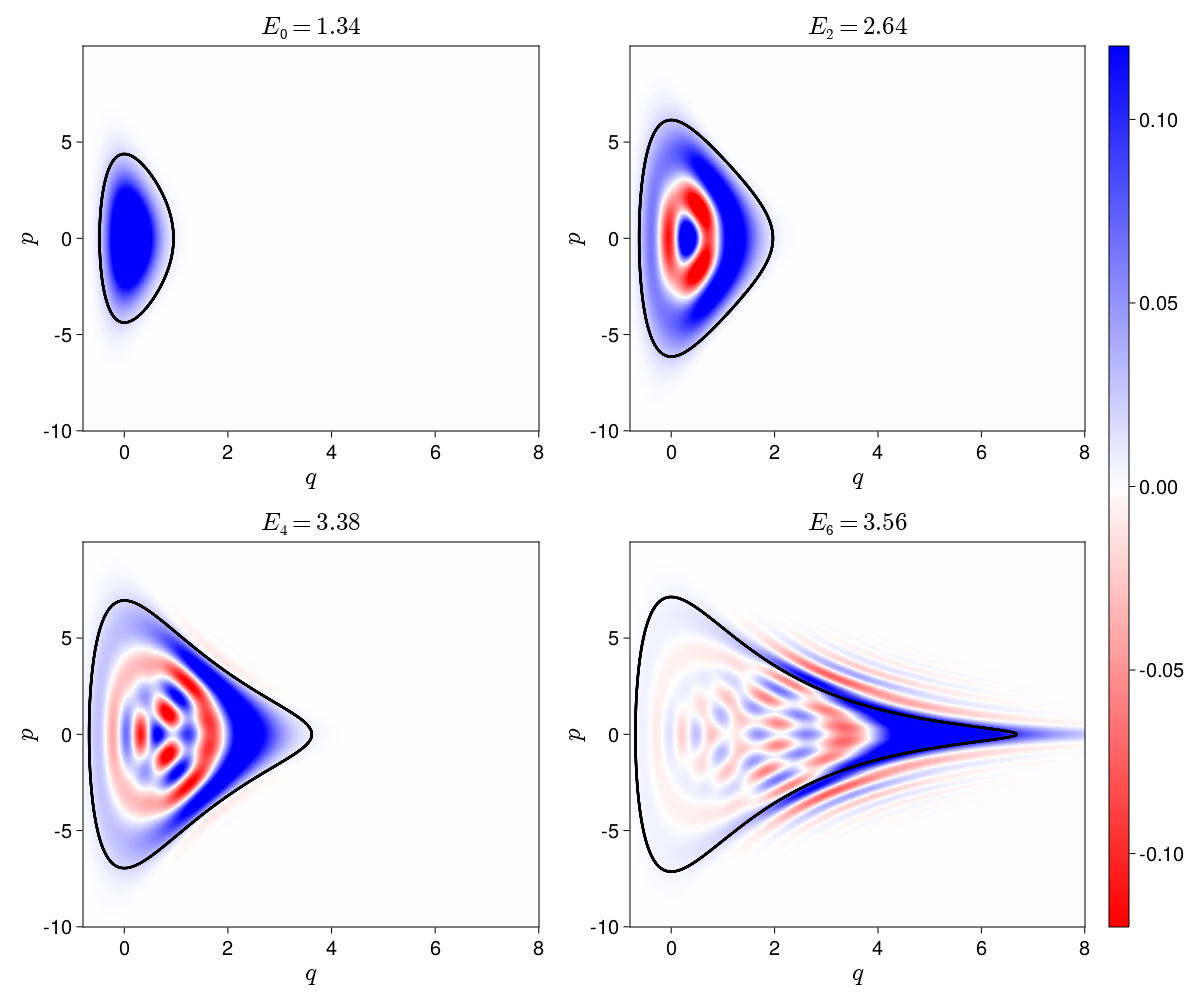
\includegraphics[width=\textwidth]{Imagens/wigner_morse.png}
    \centering
    \caption{Funções de Wigner para autoestados do sistema de Morse.}
    \label{wigner morse}
\end{figure}


\subsection{Limite Clássico}

Compararemos as aproximações semiclássicas também com o limite clássico, que possui uma expressão analítica relativamente simples. A função de partição é
\begin{equation}
    Z_{cl} = \int_R \frac{dp dq}{2\pi \hbar} e^{-\beta H(p,q)} 
\end{equation}
onde
\begin{equation}
    R = \left\{ (p,q) \ \middle| \ H(p,q) \le \frac{\hbar \omega}{4\chi}  \right\}.
\end{equation}

Definindo $P = 2\chi p/\hbar$ e $Q = 1-e^{-q}$, temos $H = \left(P^2+Q^2\right)/4\chi$ a região de integração
é expressa simplesmente por
\begin{equation}
    R = \left\{ (P,Q) \ \middle| \ P^2+Q^2 \le 1  \right\}
\end{equation}
e
\begin{equation}
    Z_{cl} = \frac{1}{4\pi\chi} \int_R \frac{dP dQ}{1-Q}  \exp \left[  -\frac{\theta \omega}{4\chi} (P^2+Q^2) \right]
\end{equation}
Introduzindo ainda coordenadas polares $Q = r \cos \phi$ e $P = r \sin \phi$, temos
\begin{equation}
    Z_{cl} = \frac{1}{4\pi\chi}\int_0^1 d r \int_0^{2\pi} d\phi  \frac{r}{1-r \cos \phi}  \exp \left[  -\frac{\theta \omega}{4\chi} r^2 \right]
\end{equation}

A integral sobre $\phi$ pode ser calculada utilizando a fórmula 3.613, 1. de \cite{gradshteyn2014table}:
\begin{equation}
    \int_0^\pi \frac{\cos nx \ dx}{1+a \cos x} = \frac{\pi}{\sqrt{1-a^2}} \left(\frac{\sqrt{1-a^2}-1}{a} \right)^n
\end{equation}
de onde obtemos
\begin{equation}
    \int_0^{2\pi} \frac{d\phi }{1-r \cos \phi} = \frac{2\pi}{\sqrt{1-r^2}}
\end{equation}
e
\begin{equation}
    Z_{cl} = \frac{1}{2\chi} \int_0^1 d r \frac{r}{\sqrt{1-r^2}} \exp \left[  -\frac{\theta \omega}{4\chi} r^2 \right]
\end{equation}
Introduzindo a variável $\rho$ tal que $\rho^2 = \theta \omega  (1-r^2)/4\chi$, chegamos a
\begin{equation}
    Z_{cl} = \frac{1}{\sqrt{\chi \theta \omega}} e^{-\theta \omega /4\chi} \int_0^{\sqrt{\theta \omega/4\chi}} e^{\rho^2} d\rho =  \frac{1}{\sqrt{\chi \theta \omega}} D_+\left(\sqrt{\theta \omega /4\chi}\right),
\end{equation}
sendo 
\begin{equation}
    D_+(u) = e^{-u^2} \int_0^{u} e^{\rho^2}d\rho
\end{equation}
a função de Dawson.

\subsection{Potencial Duplo}

No caso do sistema de Morse, o potencial modificado, definido em \eqref{potencial duplo}, é
\begin{equation}
    \begin{aligned}
        \mathbb{V}(q,y_p) &= \frac{1}{4\chi} \left( 1-2e^{-q-iy_p/2} + e^{-2q-iy_p} + 1-2e^{-q+iy_p/2} + e^{-2q+iy_p} \right) \\
        &= \frac{1}{2\chi} \left( 1-2e^{-q} \cos\frac{y_p}{2} + e^{-2q} \cos y_p \right)
    \end{aligned}
\end{equation}
de forma que as equações de movimento são
\begin{subequations}
\label{equações de movimento morse}
    \begin{equation}
        \frac{d y_p}{d \theta} = - 4\chi p
    \end{equation}
    \begin{equation}
        \frac{d y_q}{d \theta} = \frac{1}{\chi} \left( -e^{-q} \cos\frac{y_p}{2} + e^{-2q} \cos y_p \right)
    \end{equation}
    \begin{equation}
        \frac{d p}{d \theta} =  \frac{1}{2\chi} \left( e^{-q} \sin\frac{y_p}{2} - e^{-2q} \sin y_p \right)
    \end{equation}
    \begin{equation}
        \frac{d q}{d \theta} = - \chi y_q
    \end{equation}
\end{subequations}

\section{Cáusticas}

Diferente do sistema de Kerr, que estudamos anteriormente, o sistema de Morse apresenta cáusticas, que começam a surgir próximas a $\theta = 2$, de forma aparentemente independentemente de $\chi$. Na figura \ref{det part}, mostramos, na coluna da direita, o determinante jacobiano $\partial \mathbf{x}/ \partial \mathbf{X}$ como função de $\mathbf{X} = (p,q)$ para dois valores de $\theta$. Na coluna da esquerda, exibimos o integrando de \eqref{aproximação semiclassica termica} com $A(\mathbf{x})=1$, que é a expressão que utilizamos para calcular a função de partição. Podemos ver, nesse integrando, o surgimento de quase uma descontinuidade (a mudança abrupta do preto para o amarelo na esquerda do gráfico) na região que é atravessada pela cáustica, e experimentos numéricos mostram que, logo depois desse surgimento, os resultados obtidos da aproximação semiclássica afastam-se enormemente do resultado exato. 

\begin{figure}[H]
     \centering
     \begin{subfigure}[b]{\textwidth}
         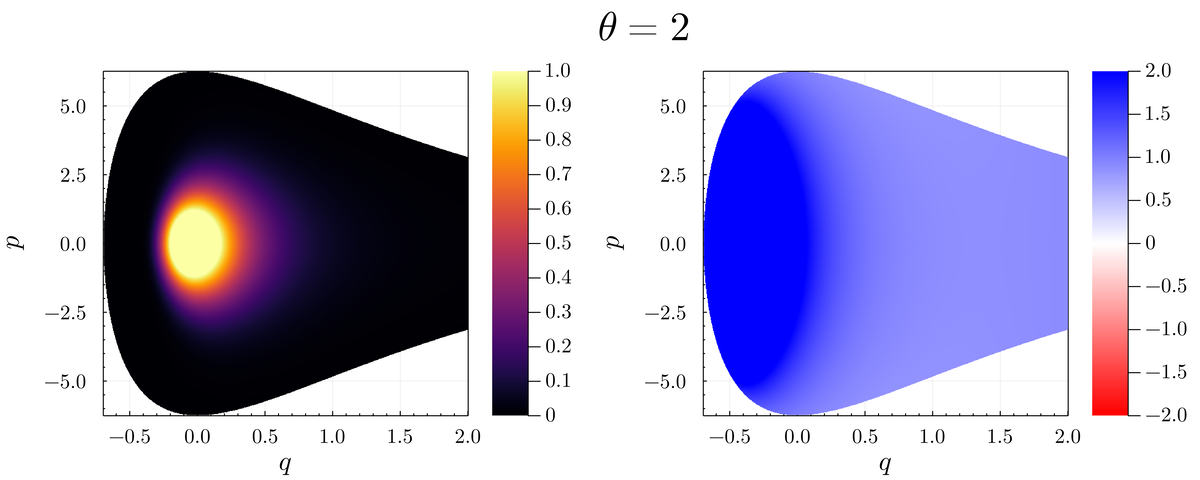
\includegraphics[width=\textwidth]{Imagens/det_part_1.png}
        \centering
    \label{det part 1}
     \end{subfigure}
     \vfill
     \begin{subfigure}[b]{\textwidth}
         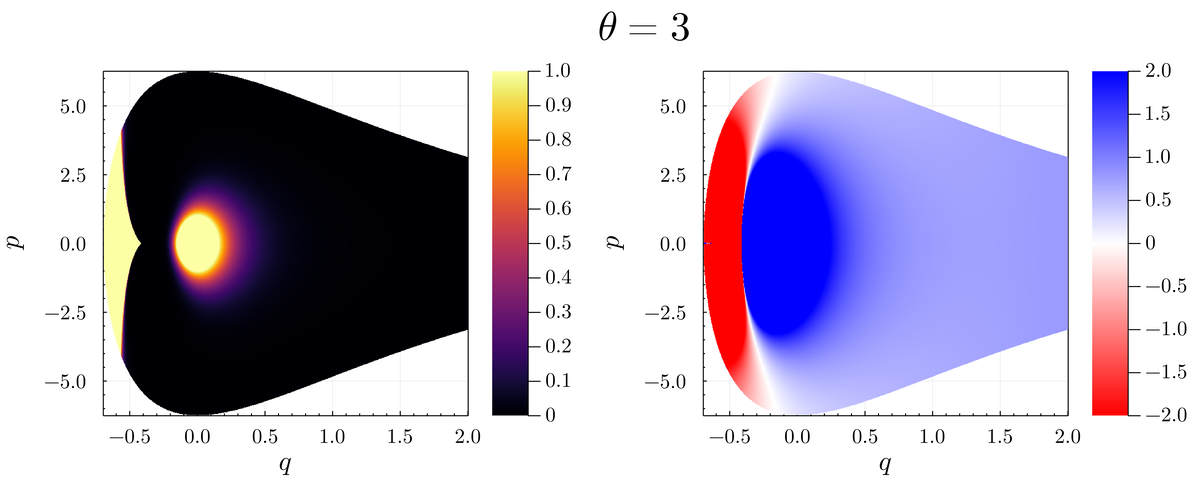
\includegraphics[width=\textwidth]{Imagens/det_part_2.png}
        \centering
    \label{det part 2}
     \end{subfigure}
        \caption{Integrando da função de partição (esquerda) e determinante jacobiano (direita) para dois valores de $\theta$. Tomamos $\chi=0.08$.}
        \label{det part}
\end{figure}

Para entender melhor o que está ocorrendo, fizemos um gráfico da ação euclidiana e do determinante jacobiano como função de $\theta$ e para um $\mathbf{X}$ fixo, que pode ser visto na figura \ref{Ação e determinante}.

\begin{figure}[H]
    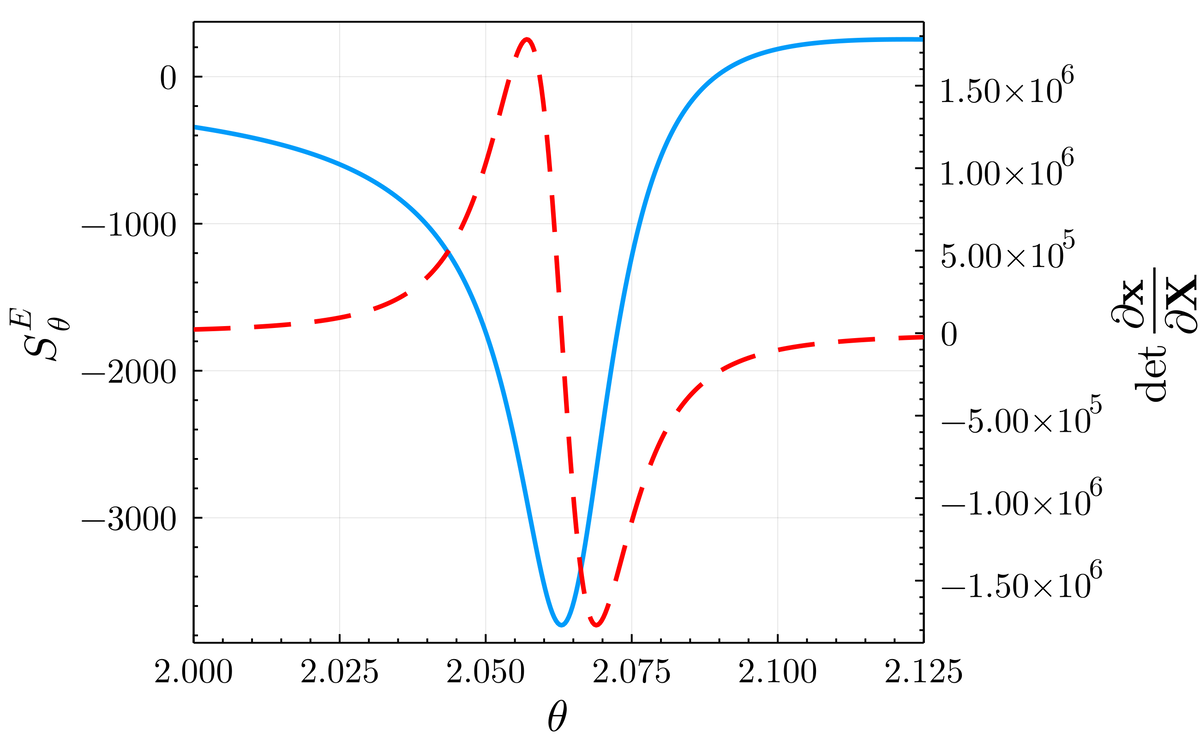
\includegraphics[width=.8\textwidth]{Imagens/ação_e_determinante.png}
    \centering
    \caption{Ação euclidiana (linha azul cheia) e determinante jacobiano (linha vermelha tracejada) próximos a $\theta=2$. Foram utilizadas as condições iniciais $p=-0.06$, $q = -0.67$. Tomamos $\chi=0.08$.}
    \label{Ação e determinante}
\end{figure}

Observa-se que, próximo à cáustica, a ação euclidiana atinge um mínimo em torno de $-4000$ e, em seguida, cresce rapidamente até um valor de $200$, o que explica a mudança abrupta observada na figura \ref{det part}. 

Como já discutido, as cáusticas são regiões sensíveis das aproximações semiclássicas, e devem ser atravessadas com cuidado. Entretanto, embora essa teoria já seja bem elucidada para tempo real \cite{de2014metaplectic}, desconhecemos como deve ser a sua adaptação no contexto de tempo imaginário. Felizmente, encontramos um truque que permite eliminar a região amarela e fornece resultados excelentes. O truque consiste simplesmente em desconsiderar uma trajetória a partir do momento que ela atravessa uma cáustica, impondo que, depois dessa travessia, sua contribuição para a integral deve se anular. Isso nos leva a crer que, seja qual for formulação teórica correta para a travessia das cáusticas com tempo imaginário, o efeito concreto dessa formulação deve ser efetivamente o que aqui descrevemos como um truque. Na figura \ref{det part 3} mostramos novamente o integrando da função de partição para $\theta = 3$, mas dessa vez com a aplicação do truque. É possível ver que a região problemática desaparece completamente.

\begin{figure}[H]
    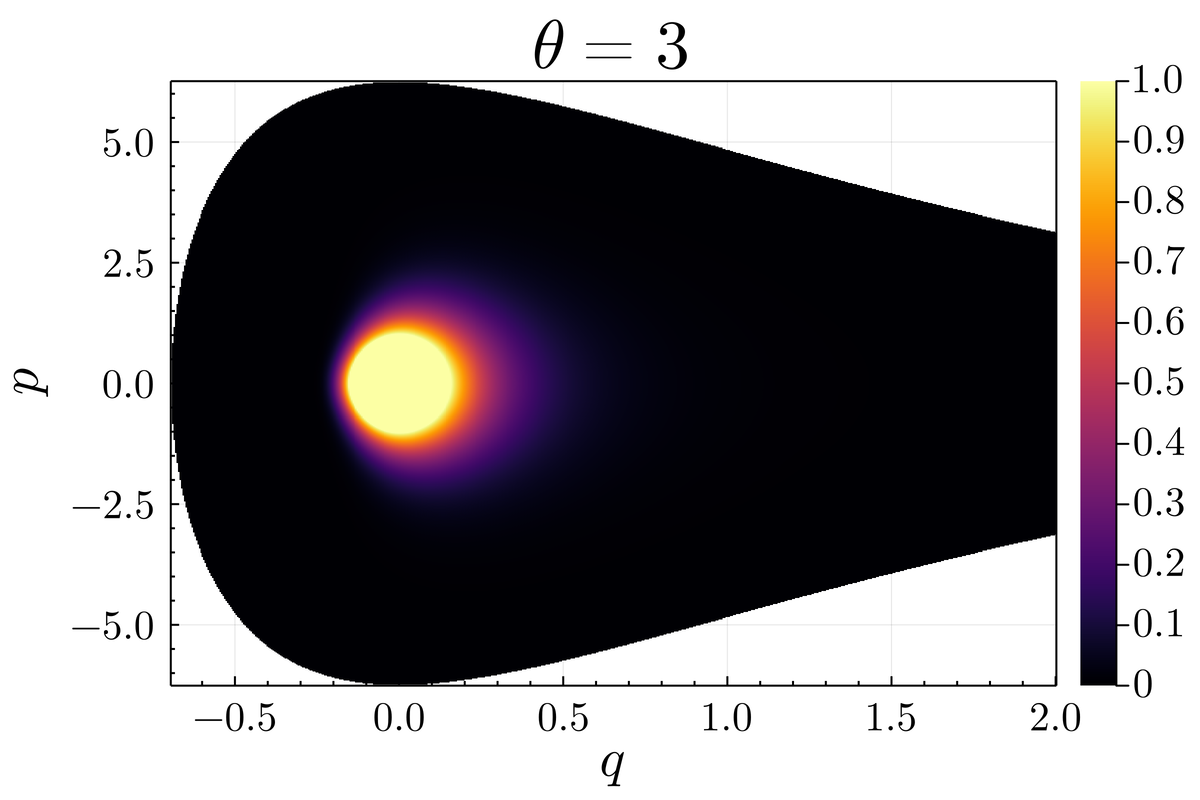
\includegraphics[width=.6\textwidth]{Imagens/det_part_3.png}
    \centering
    \caption{Integrando da função de partição corrigido pelo truque.}
    \label{det part 3}
\end{figure}

\section{Resultados Numéricos}

\subsection{Valor esperado da energia}

Repetimos aqui os mesmos gráficos feitos para o sistema de Kerr. Na figura \ref{energias morse} mostramos o valor esperado da energia como função do tempo térmico para diferentes valores de $\chi$.

\begin{figure}[H]
    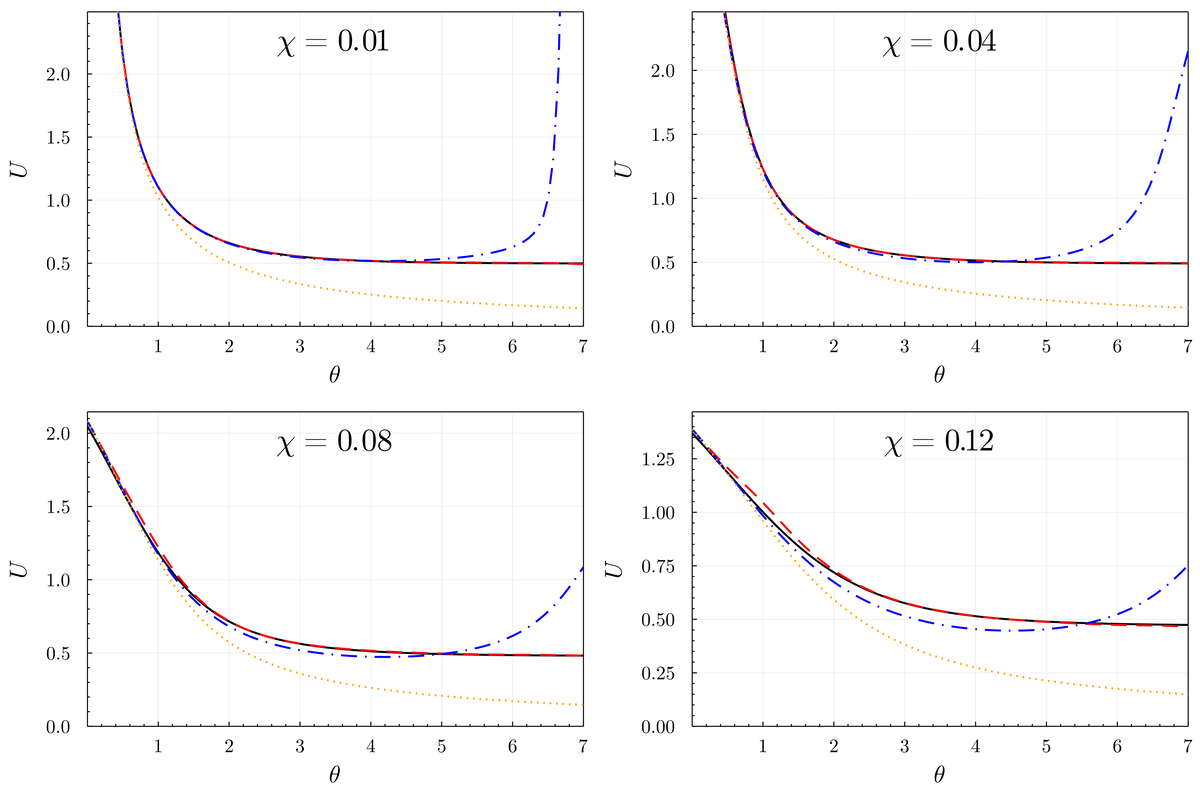
\includegraphics[width=.9\textwidth]{Imagens/energias_morse.png}
    \centering
    \caption{Energia como função do tempo térmico para diferentes valores de $\chi$. Linha preta cheia: resultado exato; linha vermelha tracejada: aproximação semiclássica, linha azul tracejada/pontilhada: aproximação metaplética amortecida; linha amarela pontilhada: resultado clássico.}
    \label{energias morse}
\end{figure}

Já na figura \ref{erros relativos morse}, mostramos o erro percentual relativo ao resultado exato para as diferentes aproximações.
\begin{figure}[H]
     \centering
     \begin{subfigure}[b]{0.32\textwidth}
         \centering
         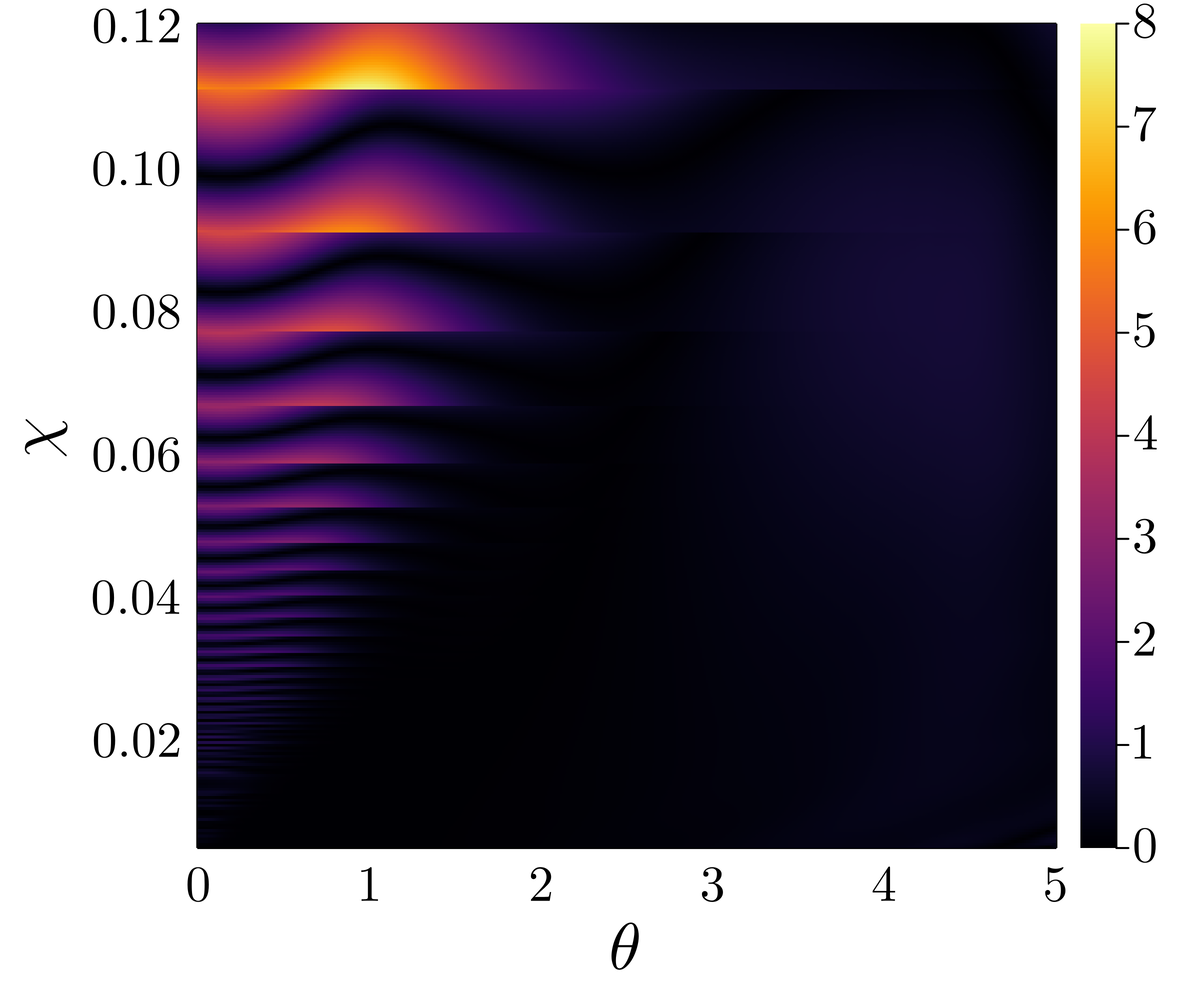
\includegraphics[width=\textwidth]{Imagens/error_sc.png}
         \caption{Semiclássica}
         \label{erro relativo morse sc}
     \end{subfigure}
     \hfill
     \begin{subfigure}[b]{0.32\textwidth}
         \centering
         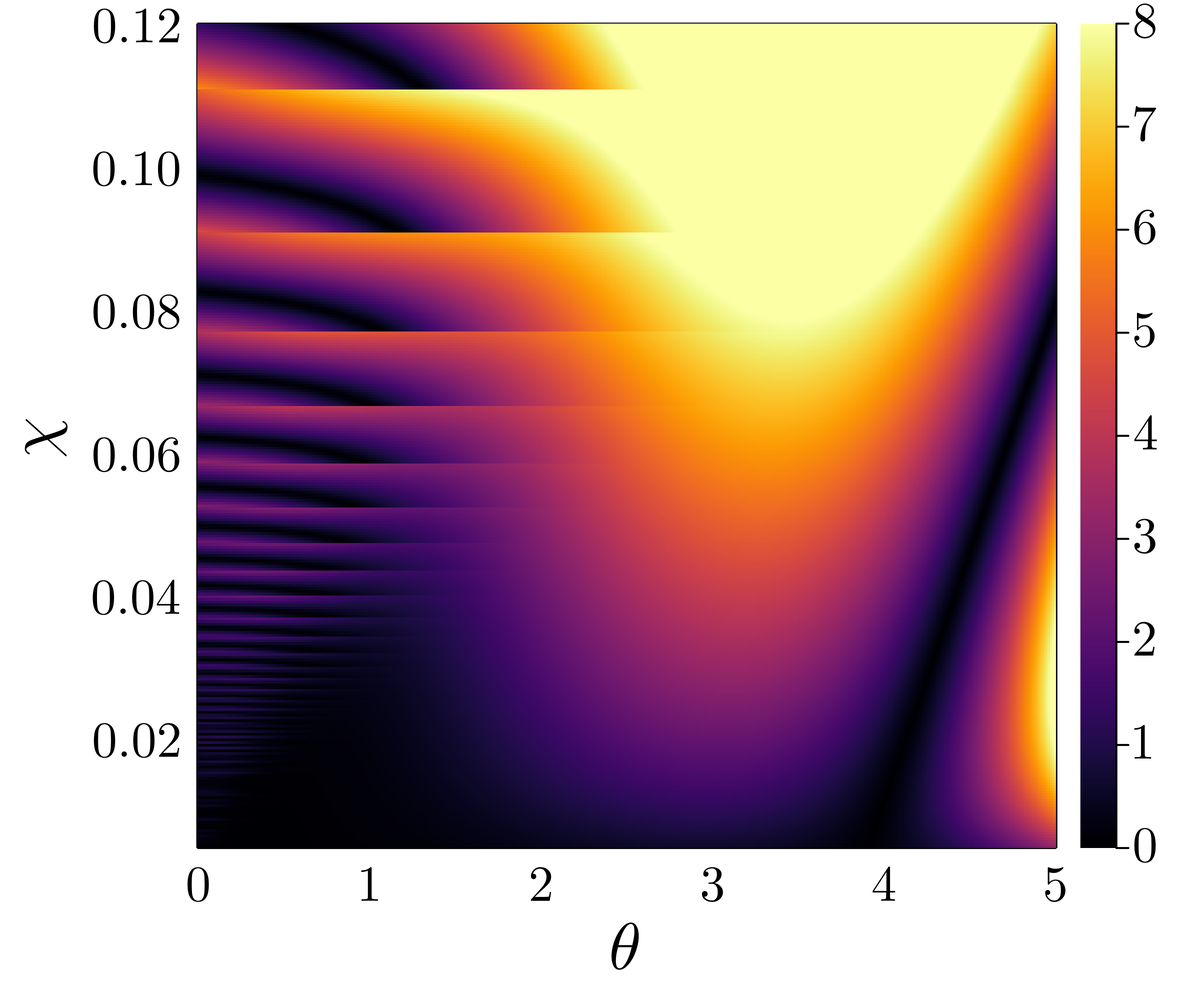
\includegraphics[width=\textwidth]{Imagens/error_dm.png}
         \caption{Metaplética Amortecida}
         \label{erro relativo morse dm}
     \end{subfigure}
     \hfill
     \begin{subfigure}[b]{0.32\textwidth}
         \centering
         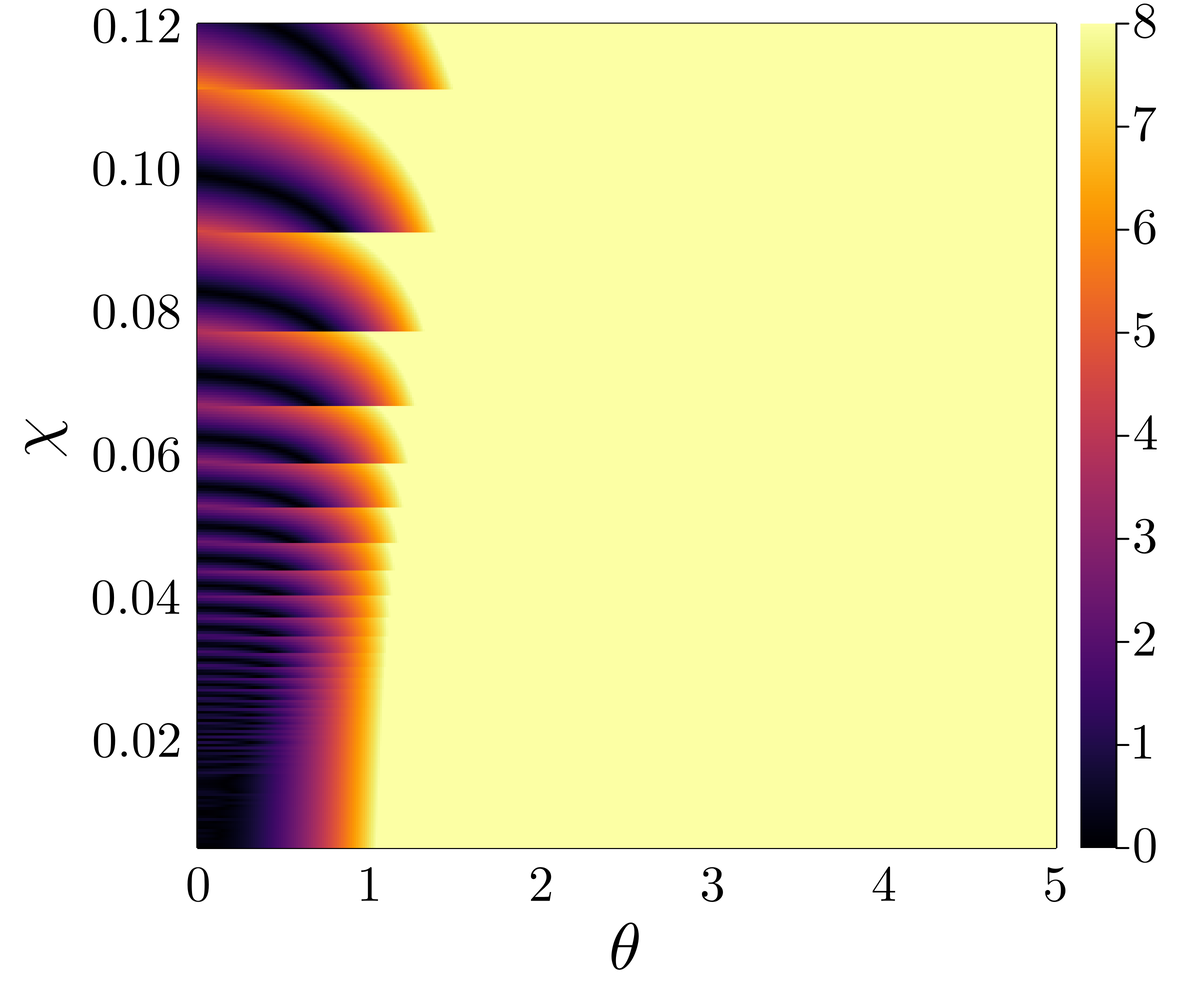
\includegraphics[width=\textwidth]{Imagens/error_cl.png}
         \caption{Clássica}
         \label{erro relativo morse cl}
     \end{subfigure}
        \caption{Erros percentuais relativos ao resultado exato como função de $\theta$ e $\chi$.}
        \label{erros relativos morse}
\end{figure}

É impressionante a qualidade da aproximação semiclássica, mesmo para os valores de $\chi$ mais altos. Observamos que, para $\chi=0.12$, temos $N=3$. Notamos ainda que, nas regiões que apresentam maior erro, isto é, aquelas com $\theta$ pequeno e $\chi$ grande, já nem devemos mais confiar no resultado que aqui chamamos de exato, uma vez que, nesse regime, os estados livres deixam de ser desprezíveis, e passariam então a influenciar as quantidades termodinâmicas fisicamente relevantes. Além disso, é exatamente nessa região na qual os estados mais excitados, cuja não convexidade é significativa, tornam-se relevantes, sendo então uma possibilidade explorar se observaríamos uma melhora da aproximação ao utilizar se utilizar a envoltória convexa como região de integração.

Observamos que as descontinuidades desse gráfico ocorrem nos pontos onde a quantidade de estados ligados quânticos muda, de acordo com \eqref{numero de estados ligados}.


\subsection{Calor Específico}

Novamente, desejamos calcular o calor específico. Agora, o quadrado da hamiltoniana toma a forma
\begin{equation}
    \hat{H}^2 = \left( \frac{\hat{p}^2}{2m} \right)^2 + V^2\left( \hat{q} \right) + V\left( \hat{q} \right)\frac{\hat{p}^2}{2m} + \frac{\hat{p}^2}{2m}V\left( \hat{q} \right)
\end{equation}
e o símbolo de Wigner correspondente pode ser obtido ao aplicar duas vezes a regra de Groenewold:
\begin{equation}
    \hat{H}^2(\mathbf{x}) = \left( \frac{p^2}{2m} \right)^2 + V^2\left( q \right) + 2V\left( q \right)\frac{p^2}{2m} - \frac{\hbar^2}{4} \frac{V''(q)}{m} = \left[ H(\mathbf{x}) \right]^2 - \left( \frac{\hbar \Omega_\mathbf{x}}{2} \right)^2,
\end{equation}
sendo $\Omega_\mathbf{x}$ exatamente como definido em \eqref{Aproximação Metaplética Amortecida padrão}.

Na figura \ref{calores morse} mostramos o calor específico $c$ como função do tempo tempo térmico $\theta$ para diferentes valores de $\chi$.

\begin{figure}[H]
    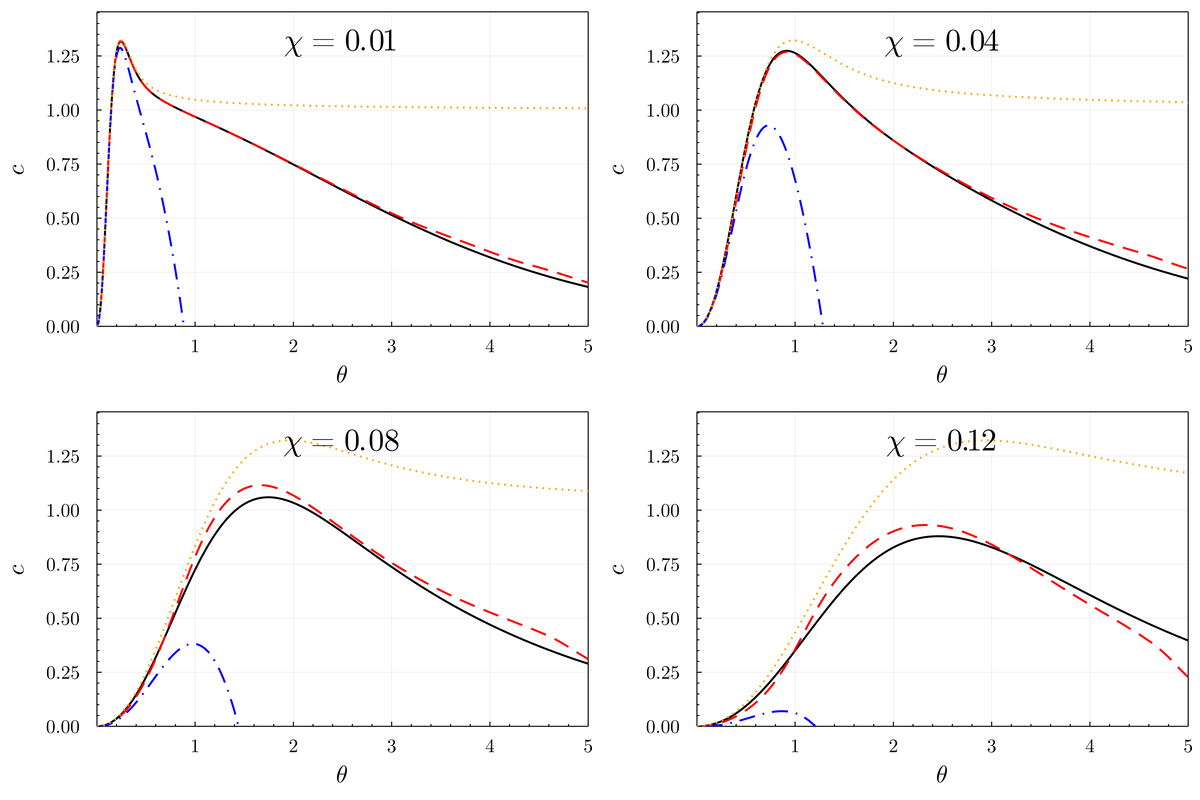
\includegraphics[width=\textwidth]{Imagens/calores_morse.png}
    \centering
    \caption{Calor específico como função do tempo térmico para diferentes valores de $\chi$. Linha preta cheia: resultado exato; linha vermelha tracejada: aproximação semiclássica, linha azul tracejada/pontilhada: aproximação metaplética amortecida; linha amarela pontilhada: resultado clássico.}
    \label{calores morse}
\end{figure}

Já na figura \eqref{erros relativos calor morse} mostramos o erro percentual relativo ao resultado exato para as diferentes aproximações.

\begin{figure}[H]
     \centering
     \begin{subfigure}[b]{0.32\textwidth}
         \centering
         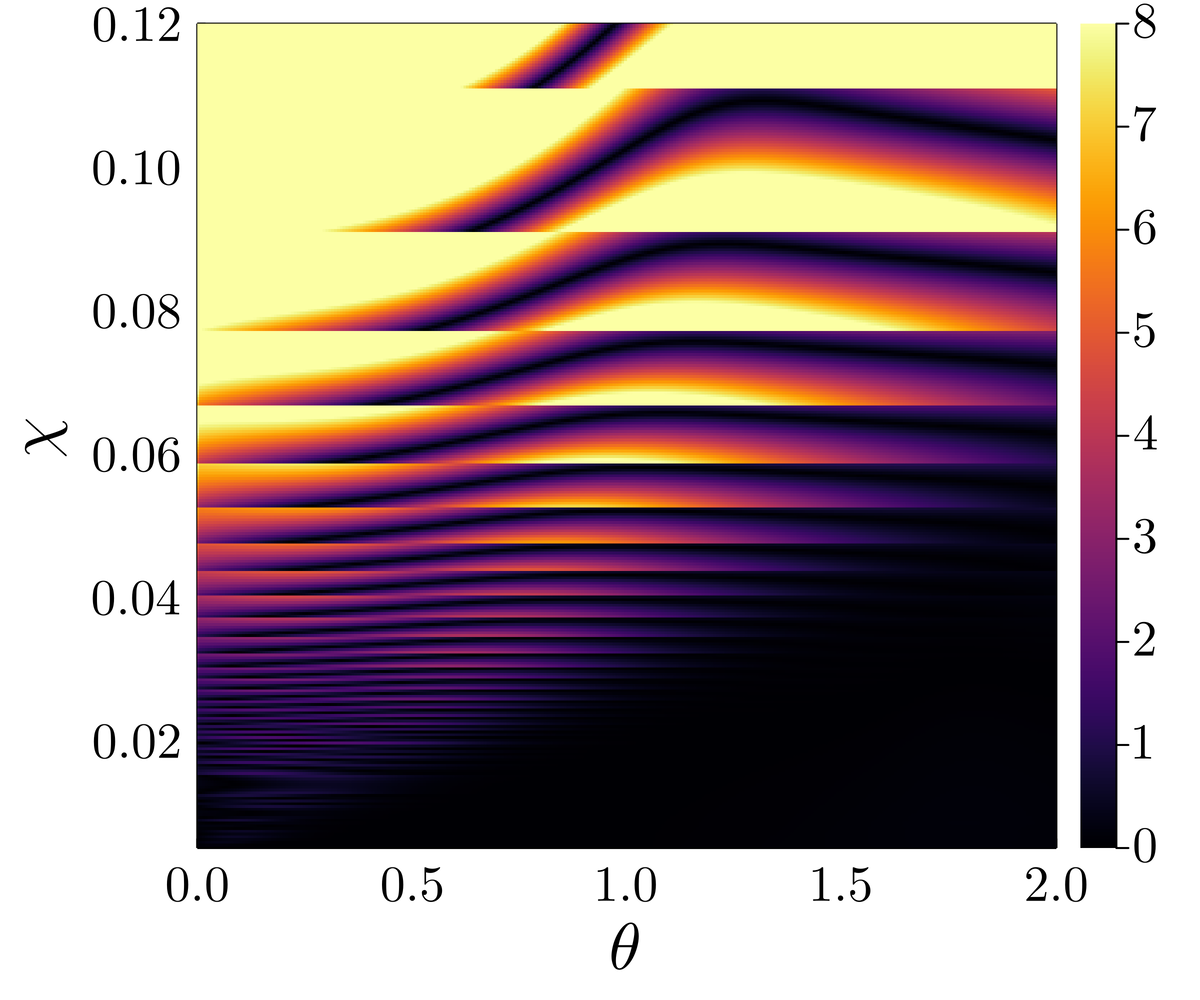
\includegraphics[width=\textwidth]{Imagens/erro_calor_sc_morse.png}
         \caption{Semiclássica}
         \label{erro relativo calor morse sc}
     \end{subfigure}
     \hfill
     \begin{subfigure}[b]{0.32\textwidth}
         \centering
         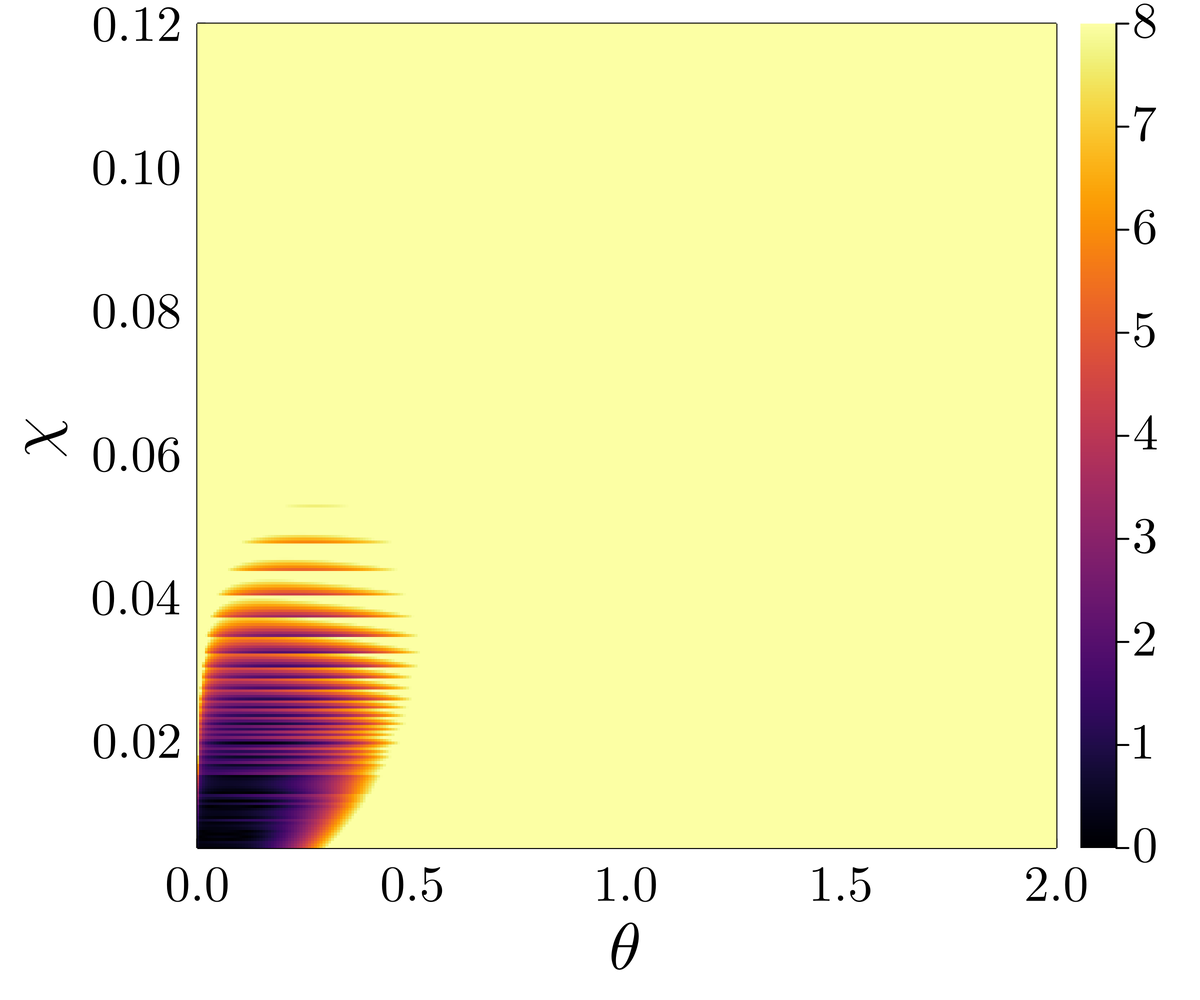
\includegraphics[width=\textwidth]{Imagens/erro_calor_dm_morse.png}
         \caption{Metaplética Amortecida}
         \label{erro relativo calor morse dm}
     \end{subfigure}
     \hfill
     \begin{subfigure}[b]{0.32\textwidth}
         \centering
         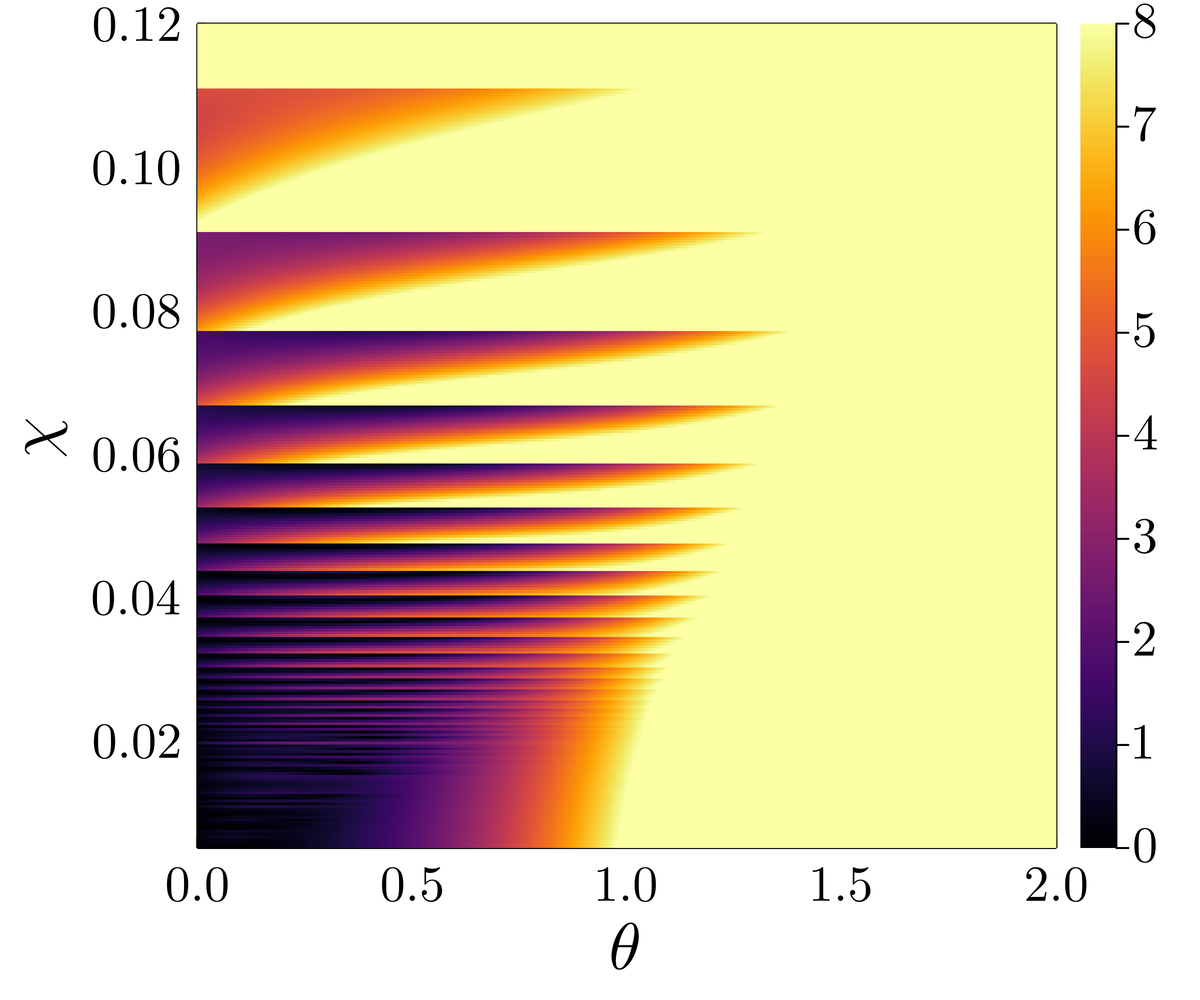
\includegraphics[width=\textwidth]{Imagens/erro_calor_cl_morse.png}
         \caption{Clássica}
         \label{erro relativo calor morse cl}
     \end{subfigure}
        \caption{Erros percentuais relativos ao resultado exato como função de $\theta$ e $\chi$.}
        \label{erros relativos calor morse}
\end{figure}

Os resultados para o sistema de Morse são, de modo qualitativo, idênticos àqueles obtidos para o sistema de Kerr — em termos de precisão, a aproximação semiclássica completa é claramente superior à metaplética amortecida, e ambas pioram quando $\chi$ cresce. Também observamos uma piora na qualidade das aproximações para o calor específico quando comparadas com as aproximações para a energia. 


\chapter{Conclusão}

Nesse trabalho estudamos aproximações semiclássicas para a função de Wigner do ensemble canônico e a utilizamos para calcular médias termodinâmicas referentes a dois sistemas de um grau de liberdades, os sistemas de Kerr e Morse. Ambos dependem de um parâmetro contínuo, que chamamos de $\chi$ nos dois casos, de forma que, quando $\chi \to 0$, os sistemas tendem ao oscilador harmônico, para os quais sabemos que a aproximação semiclássica coincide com o resultado exato. Observamos que a qualidade das aproximações piora quando $\chi$ cresce, sendo que a aproximação semiclássica completa sempre permanece mais próxima ao resultado exato, quando comparada à metaplética amortecida. Como se trata de um trabalho teórico, por um lado temos a vantagem de variar $\chi$ de maneira praticamente arbitrária, embora, por outro lado, não temos a noção da região na qual esse parâmetro é fisicamente realizável.

Para o sistema de Kerr, que é uma forma normal de Birkhoff, e que, portanto, nos permite obter uma expressão exata para a ação, podemos checar que a aproximação semiclássica tende ao resultado exato tanto para baixas quanto para altas temperaturas, e que a qualidade na região intermediária depende do valor de $\chi$.

Além disso, discutimos em certo detalhe sistemas com uma hamiltoniana padrão, incluindo o caso no qual o potencial é limitado, e portanto, admite também estados livres. Para calcular as médias termodinâmicas em um regime de temperatura abaixo do limiar dos estados livres, apresentamos a prescrição clássica, que consiste em realizar as integrações relevantes apenas na região classicamente permitida, e, analisando, a construção das funções de Wigner semiclássicas feitas em \cite{berry1977semi}, propomos uma correção semiclássica a essa prescrição, que consiste em realizar as integrais na envoltória convexa da região classicamente permitida, embora a avaliação numérica de tal proposta ainda não tenha sido feita. Para o sistema de Morse, em particular, é possível ver que nos valores fisicamente realizáveis do parâmetro $\chi$, a aproximação semiclássica obteve resultados excelentes.

A aproximação metaplética amortecida, como apresentada aqui, é restrita ao caso de um grau de liberdade, mas a aproximação semiclássica completa é, em tese, diretamente generalizável para mais graus de liberdade, bastando, do ponto de vista da implementação computacional, encontrar uma forma adequada de realizar as integrações, o que provavelmente pode ser feito por algum método Monte Carlo. Restaria então encontrar algum sistema físico concreto, para testar se seus parâmetros estão dentro da região na qual a aproximação é boa. Seria para esses sistemas grandes, para os quais a obtenção de níveis de energia é uma tarefa extremamente custosa, que supomos que nossa aproximação semiclássica tenha uma aplicação real.

\postextual

\begin{apendicesenv}

\chapter{Polígonos no espaço de fase}
\label{apendice_area}

Nesse apêndice, discutiremos algumas propriedades geométricas relacionadas a polígonos no espaço de fase, que são utilizadas em diversos momentos ao longo deste trabalho. Estaremos interessados, mais especificamente, nas propriedades da área $\Delta_{N+1}\left(\mathbf{x},\mathbf{x}_1,\ldots,\mathbf{x}_{N}\right)$ de um polígono cujos $N+1$ lados estão centrados em $\mathbf{x},\mathbf{x}_1,\ldots,\mathbf{x}_{N}$.

Primeiramente, observamos que, quando $N$ é ímpar, é sempre possível expressar um dos centros em termos dos demais, isto é, eles não são independentes. Para ver isso, podemos analisar, por exemplo, o quadrilátero da figura \ref{quadrilatero}.
\begin{figure}[H]
    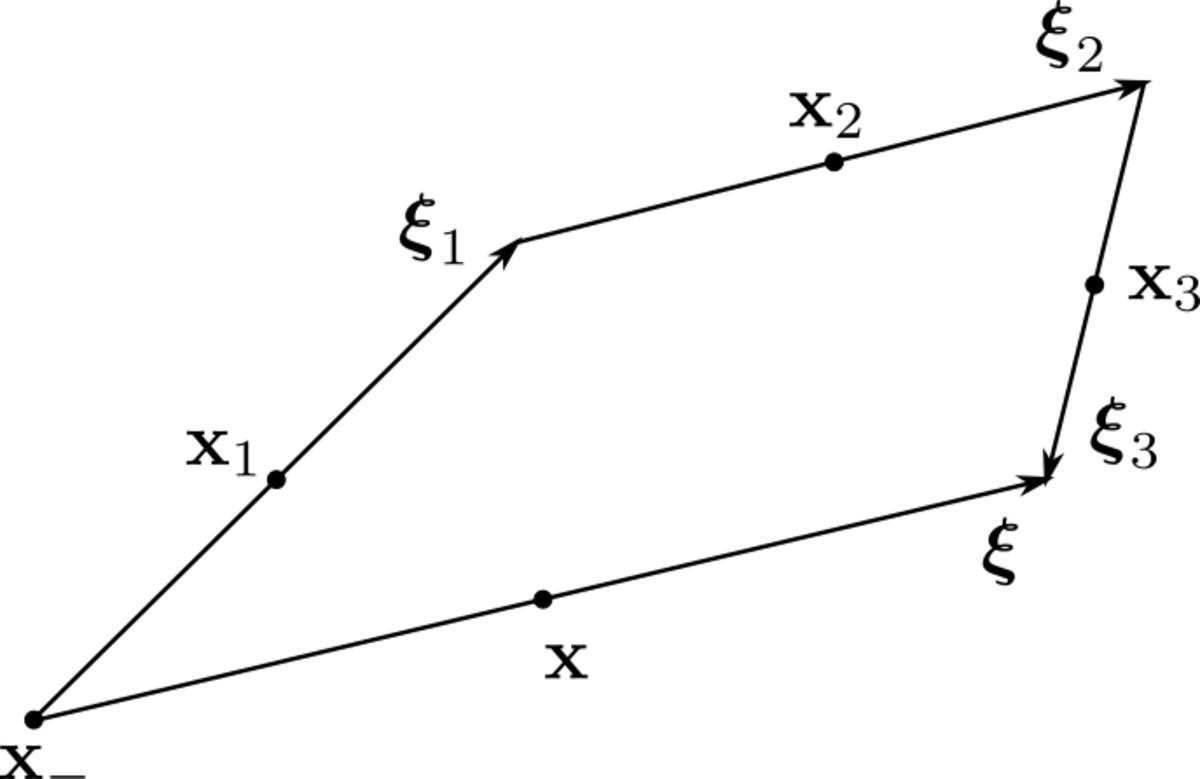
\includegraphics[width=.6\textwidth]{Imagens/quadrilatero.png}
    \centering
    \caption{Um quadrilátero no espaço de fase}
    \label{quadrilatero}
\end{figure}

Vemos que valem as relações
\begin{align*}
     \mathbf{x}_1 &= \mathbf{x}_- + \frac{1}{2}\boldsymbol{\xi}_1 \Label{onea}& \mathbf{x}_{2}&= \mathbf{x}_- + \boldsymbol{\xi}_1 + \frac{1}{2}\boldsymbol{\xi}_2 \Label{twoa}\\
     \mathbf{x} &= \mathbf{x}_- + \frac{1}{2}\boldsymbol{\xi} \Label{threea}& \mathbf{x}_{3}&=\mathbf{x}_- + \boldsymbol{\xi} - \frac{1}{2}\boldsymbol{\xi}_3 \Label{foura}
\end{align*}
de onde obtemos
\begin{equation}
\label{relação paralelogramo}
    \mathbf{x} - \mathbf{x}_1 + \mathbf{x}_2 - \mathbf{x}_3 = \boldsymbol{0}.
\end{equation}
Essa expressão pode ser interpretada ao considerar que o quadrilátero é obtido através da composição de três reflexões, em torno dos centros $\mathbf{x}_1$, $\mathbf{x}_2$ e $\mathbf{x}_3$. Das relações \eqref{reflexões e translações clássicas}, vemos que o resultado dessa composição é também uma reflexão, cujo centro é precisamente $\mathbf{x} = \mathbf{x}_1 - \mathbf{x}_2 + \mathbf{x}_3$. No caso da composição de um número par de reflexões, o mesmo não ocorre, tendo em vista que o resultado é uma translação, que, portanto, deixa livre o último centro.

Será útil para nós a obtenção da área do quadrilátero, o que pode ser feito ao decompô-lo em dois triângulos, como na figura \ref{decomposição_quadrilatero}.
\begin{figure}[H]
    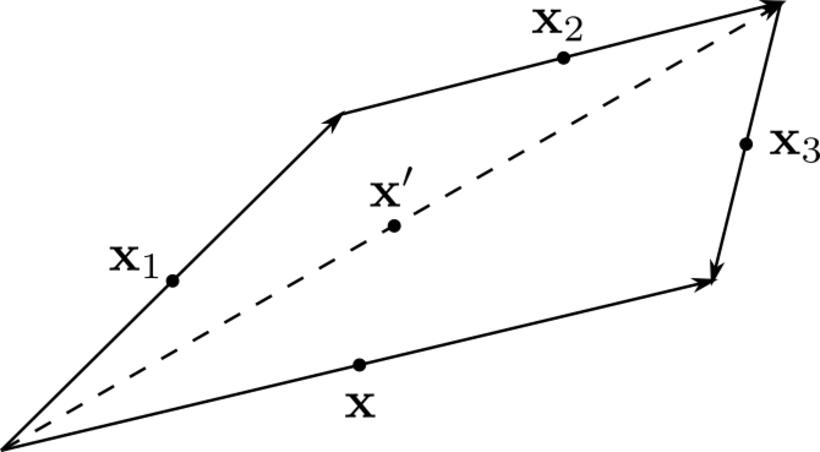
\includegraphics[width=.6\textwidth]{Imagens/decomposição_quadrilatero.png}
    \centering
    \caption{Decomposição de um quadrilátero como dois triângulos}
    \label{decomposição_quadrilatero}
\end{figure}

Com isso, temos
\begin{equation}
    \label{desenvolvimento area quadrilatero}
    \begin{aligned}
        \Delta_4\left(\mathbf{x},\mathbf{x}_1,\mathbf{x}_2,\mathbf{x}_3 \right) & = \Delta_3\left(\mathbf{x}',\mathbf{x}_1,\mathbf{x}_2\right) + \Delta_3\left(\mathbf{x},\mathbf{x}',\mathbf{x}_3 \right) \\ &=  \mathbf{x}' \wedge \left( \mathbf{x}_1 - \mathbf{x}_2 + \mathbf{x}_3 - \mathbf{x} \right) + \mathbf{x}_1 \wedge \mathbf{x}_2  + \mathbf{x}_3 \wedge \mathbf{x}  \\ &= \mathbf{x}_1 \wedge \mathbf{x}_2 + \mathbf{x}_3 \wedge \mathbf{x},
    \end{aligned}
\end{equation}
sendo que, na última igualdade, utilizamos \eqref{relação paralelogramo} para concluir que os termos contendo $\mathbf{x}'$ se anulam. Além disso, como já mencionado, os centros não são independentes, de forma que, utilizando \eqref{relação paralelogramo} novamente, podemos, por exemplo, expressar $\mathbf{x}_1$ em termos dos demais centros, de onde obtemos
\begin{equation}
\label{quadrilatero como triangulo}
    \begin{aligned}
        \Delta_4\left(\mathbf{x},\mathbf{x}_1,\mathbf{x}_2,\mathbf{x}_3 \right) &= \left( \mathbf{x}_2 - \mathbf{x}_3 + \mathbf{x} \right) \wedge \mathbf{x}_2 + \mathbf{x}_3 \wedge \mathbf{x} \\
        &= \mathbf{x}  \wedge \mathbf{x}_2 + \mathbf{x}_2 \wedge \mathbf{x}_3 + \mathbf{x}_3 \wedge \mathbf{x} = \Delta_3 \left( \mathbf{x}, \mathbf{x}_2,\mathbf{x}_3 \right),
    \end{aligned}
\end{equation}
isto é, a área do quadrilátero é idêntica a área de um triângulo que compartilha três dos seus centros.

Esse resultado pode ser utilizado para obter as derivadas de $\Delta$ em relação aos centros. Mais precisamente, mostraremos que, sendo $\Delta_{2n+1}\left(\mathbf{x},\mathbf{x}_1,\ldots,\mathbf{x}_{2n}\right)$ a área de um polígono cujos lados estão centrados em $\mathbf{x},\mathbf{x}_1,\ldots,\mathbf{x}_{2n}$, vale
\begin{equation}
    \label{derivadas área}
    \frac{\partial \Delta_{2n+1}}{\partial \mathbf{x}_j} = - \mathbf{J} \boldsymbol{\xi}_j, \ \ \ j = 1,\ldots,2n; \ \ \ \ \frac{\partial \Delta_{2n+1}}{\partial \mathbf{x}} = \mathbf{J} \boldsymbol{\xi},
\end{equation}
sendo $\boldsymbol{\xi}_j$ o lado corresponde ao centro $\mathbf{x}_j$ e $\boldsymbol{\xi} = \sum_j \boldsymbol{\xi}_j$. Nossa estratégia é utilizar uma prova por indução sobre $n$, sendo que o caso $n=1$ já foi discutido na seção \ref{composição funções geratrizes}. Faremos então a suposição de que \eqref{derivadas área} é válido para um certo $n$ e utilizaremos esta hipótese para mostrar que o resultado continua válido para $n+1$.

Consideraremos um polígono de lados centrados em $\mathbf{x},\mathbf{x}_1,\ldots,\mathbf{x}_{2n+2}$, ilustrado na figura \ref{poligono grande}, cuja a área é $\Delta_{2n+3}\left(\mathbf{x},\mathbf{x}_1,\ldots,\mathbf{x}_{2n+2}\right)$. Também marcamos na figura os centros auxiliares $\mathbf{x}'$ e $\mathbf{x}''$.

\begin{figure}[H]
    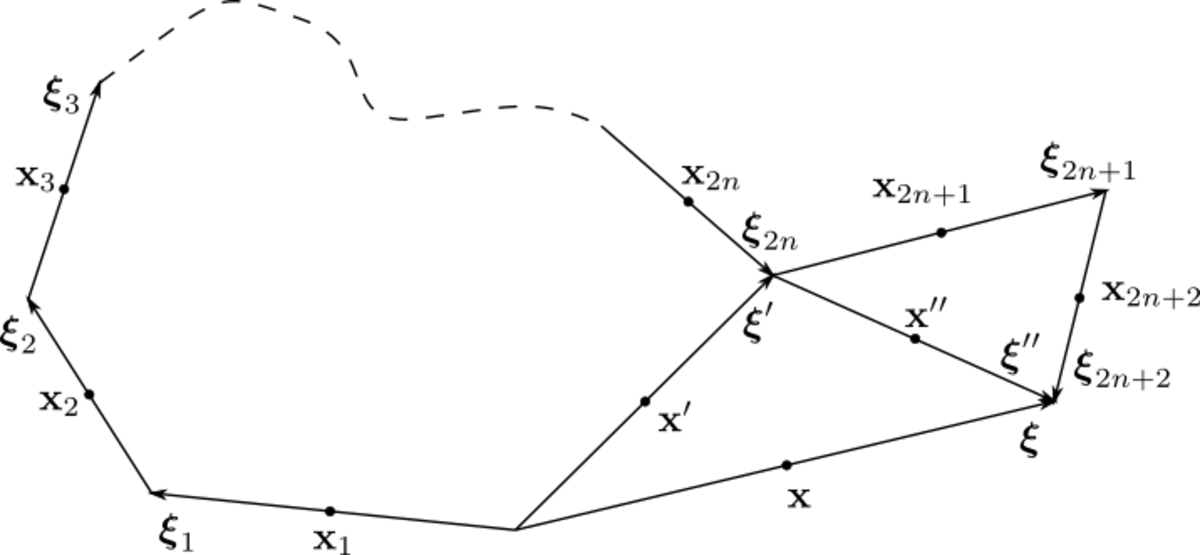
\includegraphics[width=.8\textwidth]{Imagens/n_gon.png}
    \centering
    \caption{Decomposição da área de um polígono de $2n+3$ lados}
    \label{poligono grande}
\end{figure}

Utilizando \eqref{quadrilatero como triangulo}, temos
\begin{equation}
\label{delta 2n+3}
    \begin{aligned}
        \Delta_{2n+3}\left(\mathbf{x},\mathbf{x}_2,\ldots,\mathbf{x}_{2n+2}\right) &=  \Delta_{2n+1}\left(\mathbf{x}',\mathbf{x}_2,\ldots,\mathbf{x}_{2n}\right)+\Delta_4 \left(\mathbf{x}, \mathbf{x}', \mathbf{x}_{2n+1},\mathbf{x}_{2n+2}\right)\\&=  \Delta_{2n+1}\left(\mathbf{x}',\mathbf{x}_2,\ldots,\mathbf{x}_{2n}\right)+\Delta_3 \left(\mathbf{x},\mathbf{x}_{2n+1},\mathbf{x}_{2n+2}\right),
    \end{aligned}
\end{equation}
sendo
\begin{equation}
\label{xis linha}
    \mathbf{x}' = \mathbf{x}  + \mathbf{x}_{2n+1} - \mathbf{x}_{2n+2}
\end{equation}
de acordo com \eqref{relação paralelogramo}.

Para prosseguir, precisaremos expressar as derivadas de $\Delta_3$ de forma conveniente. Para isso, notamos que, desta vez, valem as relações
\begin{align*}
     \mathbf{x}'' - \mathbf{x}' &= \frac{1}{2}\boldsymbol{\xi} \Label{one}& \mathbf{x}_{2n+2} - \mathbf{x}_{2n+1} &= \frac{1}{2}\boldsymbol{\xi}'' \Label{two}\\
     \mathbf{x}'' - \mathbf{x} &= \frac{1}{2}\boldsymbol{\xi}' \Label{three}& \mathbf{x}_{2n+2} - \mathbf{x}'' &= \frac{1}{2}\boldsymbol{\xi}_{2n+1} \Label{four} \\
     \mathbf{x} - \mathbf{x}' &= \frac{1}{2}\boldsymbol{\xi}'' \Label{five}& \mathbf{x}'' - \mathbf{x}_{2n+1} &= \frac{1}{2}\boldsymbol{\xi}_{2n+2} \Label{six}
\end{align*}

Combinando \eqref{three} e \eqref{four} obtemos
\begin{equation}
    \frac{\partial \Delta_3}{\partial \mathbf{x}_{2n+1}} = 2\mathbf{J}\left(\mathbf{x}-\mathbf{x}_{2n+2}\right) = - \mathbf{J}\left( \boldsymbol{\xi}' + \boldsymbol{\xi}_{2n+1} \right),
\end{equation}
a partir de \eqref{three} e \eqref{six}, chegamos a
\begin{equation}
    \frac{\partial \Delta_3}{\partial \mathbf{x}_{2n+1}} = 2 \mathbf{J} \left(\mathbf{x}_{2n+2}-\mathbf{x}\right) = \mathbf{J}\left( \boldsymbol{\xi}' - \boldsymbol{\xi}_{2n+2} \right),
\end{equation}
e, por fim, utilizando \eqref{two},
\begin{equation}
    \frac{\partial \Delta_3}{\partial \mathbf{x}} = 2 \mathbf{J} \left(\mathbf{x}_{2n+2}-\mathbf{x}_{2n+1}\right) = \mathbf{J}\boldsymbol{\xi}''.
\end{equation}

Para concluir o argumento, utilizamos a hipótese de indução, que nos diz que
\begin{equation}
    \frac{\partial \Delta_{2n+1}}{\partial \mathbf{x}_j} = - \mathbf{J} \boldsymbol{\xi}_j, \ \ \ j = 1,\ldots,2n; \ \ \ \ \frac{\partial \Delta_{2n+1}}{\partial \mathbf{x}'} = \mathbf{J} \boldsymbol{\xi}',
\end{equation}
e, então,
\begin{equation}
    \frac{\partial \Delta_{2n+3}}{\partial \mathbf{x}_j} = - \mathbf{J} \boldsymbol{\xi}_j, \ \ \ j = 1,\ldots,2n.
\end{equation}

A derivada em relação aos demais centros fica
\begin{equation}
    \frac{\partial \Delta_{2n+3}}{\partial \mathbf{x}_{2n+1}} = \frac{\partial \Delta_{2n+1}}{\partial \mathbf{x}'} \frac{\partial \mathbf{x}'}{\mathbf{x}_{2n+1}} + \frac{\partial \Delta_3}{\partial \mathbf{x}_{2n+1}} =- \mathbf{J} \boldsymbol{\xi}_{2n+1}
\end{equation}

\begin{equation}
    \frac{\partial \Delta_{2n+3}}{\partial \mathbf{x}_{2n+2}} = \frac{\partial \Delta_{2n+1}}{\partial \mathbf{x}'} \frac{\partial \mathbf{x}'}{\mathbf{x}_{2n+2}} + \frac{\partial \Delta_3}{\partial \mathbf{x}_{2n+2}} = -\mathbf{J} \boldsymbol{\xi}_{2n+2}
\end{equation}

\begin{equation}
    \frac{\partial \Delta_{2n+3}}{\partial \mathbf{x}} = \frac{\partial \Delta_{2n+1}}{\partial \mathbf{x}'} \frac{\partial \mathbf{x}'}{\mathbf{x}} + \frac{\partial \Delta_3}{\partial \mathbf{x}} = \mathbf{J}\left(\boldsymbol{\xi}'+\boldsymbol{\xi}''\right) = \mathbf{J}\boldsymbol{\xi},
\end{equation}
o que completa o argumento.

Por fim, queremos discutir o efeito de variações nos centros sobre a área do paralelogramo, isto é, queremos obter
\begin{equation}
    \Delta_{N+1}\left(\mathbf{x} + \delta\mathbf{x},\mathbf{x}_1+\delta\mathbf{x}_1,\ldots,\mathbf{x}_{N}+\delta\mathbf{x}_N\right).
\end{equation}
Como vimos neste apêndice, em geral, podemos escrever
\begin{equation}
    \Delta_{N+1}\left(\mathbf{x},\mathbf{x}_1,\ldots,\mathbf{x}_{N}\right) = \sum_{j,k=0}^N d_{jk} \mathbf{x}_j \wedge \mathbf{x}_k
\end{equation}
para certos coeficientes constantes $d_{jk}$, e, para fim de indexação, convencionamos $\mathbf{x}_0 = \mathbf{x}$. Isso mostra que
\begin{equation}
    \begin{aligned}
        &\Delta_{N+1}\left(\mathbf{x} + \delta\mathbf{x},\mathbf{x}_1+\delta\mathbf{x}_1,\ldots,\mathbf{x}_{N}+\delta\mathbf{x}_N\right)\\  =& \sum_{j,k=0}^N d_{jk} \mathbf{x}_j \wedge \mathbf{x}_k + \sum_{j,k=0}^N d_{jk} \mathbf{x}_j \wedge \delta\mathbf{x}_k + \sum_{j,k=0}^N d_{jk} \delta\mathbf{x}_j \wedge \mathbf{x}_k + \sum_{j,k=0}^N d_{jk} \delta\mathbf{x}_j \wedge \delta\mathbf{x}_k \\ =& \ \Delta_{N+1}\left(\mathbf{x},\mathbf{x}_1,\ldots,\mathbf{x}_{N}\right)  + \sum_{j,k=0}^N d_{jk} \mathbf{x}_j \wedge \delta\mathbf{x}_k \\ &+ \sum_{j,k=0}^N d_{jk} \delta\mathbf{x}_j \wedge \mathbf{x}_k + \Delta_{N+1}\left( \delta\mathbf{x},\delta\mathbf{x}_1,\ldots,\delta\mathbf{x}_N\right),
    \end{aligned}
\end{equation}
Os termos lineares nos $\delta \mathbf{x}_j$ podem ser ainda reescritos de forma conveniente ao observar que devem coincidir com o termo de ordem $1$ da série de Taylor de $\Delta_{N+1}$ em torno de $\left(\mathbf{x},\mathbf{x}_1,\ldots,\mathbf{x}_{N}\right)$. Como as derivadas de primeira ordem, pelo menos no caso em que $N$ é par, são dadas por \eqref{derivadas área}, obtemos
\begin{equation}
    \label{variação área}
    \begin{aligned}
        &\Delta_{N+1}\left(\mathbf{x} + \delta\mathbf{x},\mathbf{x}_1+\delta\mathbf{x}_1,\ldots,\mathbf{x}_{N}+\delta\mathbf{x}_N\right) \\
    &=\Delta_{N+1}\left(\mathbf{x},\mathbf{x}_1,\ldots,\mathbf{x}_{N}\right)  + \mathbf{J} \boldsymbol{\xi} \cdot \delta\mathbf{x}  - \sum_{j=1}^N \mathbf{J} \boldsymbol{\xi}_j \cdot \delta\mathbf{x}_j  + \Delta_{N+1}\left( \delta\mathbf{x},\delta\mathbf{x}_1,\ldots,\delta\mathbf{x}_N\right).
    \end{aligned}
\end{equation}

\chapter{Cálculo do termo de área}
\label{Cálculo do termo de área}
Utilizando o teorema de Green, mostra-se que a área da região envolta por uma curva fechada $\gamma:[a,b]\to\mathbb{R}^2$ pode ser calculada por
\begin{equation}
    \Delta = \frac{1}{2}\int_a^b \gamma_p(s) \gamma'_q(s) -  \gamma'_p(s) \gamma_q(s) ds,
\end{equation}
sendo $\gamma(s) = (\gamma_p(s),\gamma_q(s))$.

No caso particular da área entre a trajetória e a corda, decompomos $\gamma$ como $\gamma = \gamma_1  - \gamma_2 - \gamma_3$, como ilustrado na figura \eqref{curva para calculo da área}, sendo
\begin{subequations}
    \begin{equation}
        \begin{aligned}
            \gamma_1 \colon[0,t/2] &\to \mathbb{R}^2\\
            t' &\mapsto  \mathbf{x}(t') + \frac{1}{2}\boldsymbol{\xi}(t')
    \end{aligned}
    \end{equation}
    \begin{equation}
        \begin{aligned}
            \gamma_2 \colon[0,t/2] &\to \mathbb{R}^2\\
            t' &\mapsto  \mathbf{x}(t') - \frac{1}{2}\boldsymbol{\xi}(t')
    \end{aligned}
    \end{equation}
    \begin{equation}
        \begin{aligned}
            \gamma_3 \colon[-1/2,1/2]
             &\to \mathbb{R}^2\\
            \lambda &\mapsto  \mathbf{x}(t/2) + \lambda \boldsymbol{\xi}(t/2)
    \end{aligned}
    \end{equation}
\end{subequations}

\begin{figure}[H]
    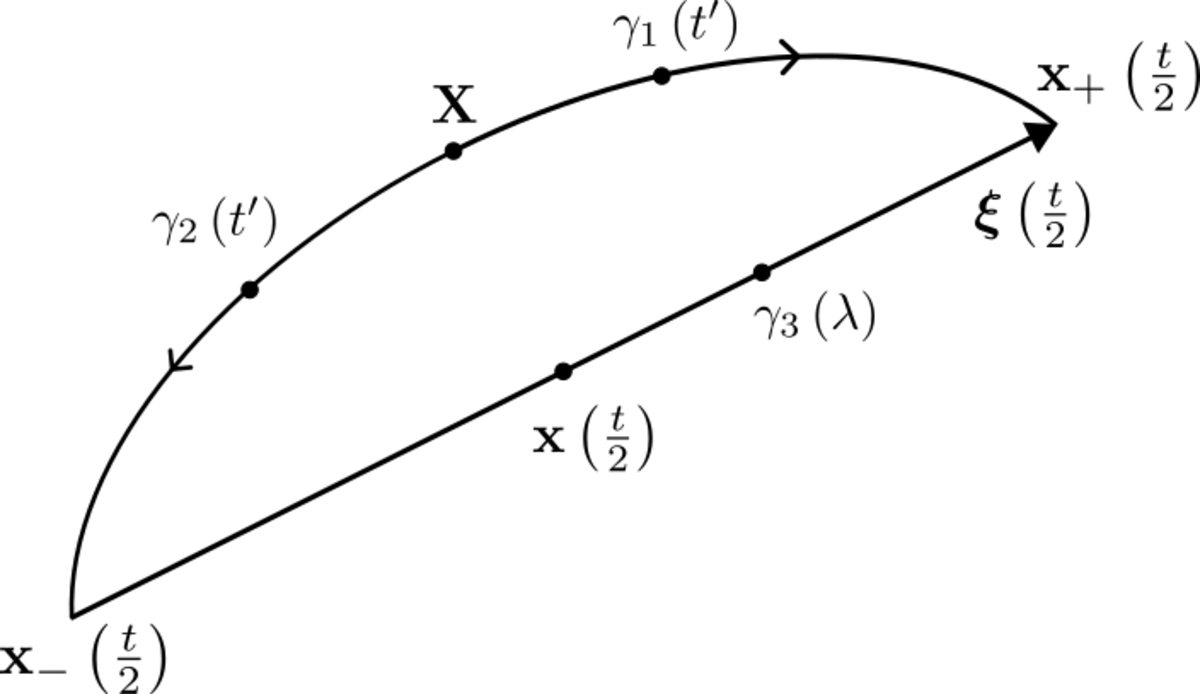
\includegraphics[width=.6\textwidth]{Imagens/half_trajectories_v2.png}
    \centering
    \caption{Curvas utilizadas para o cálculo de $\Delta$.}
    \label{curva para calculo da área}
\end{figure}

Temos
\begin{equation}
    \begin{aligned}
        &\int_{\gamma_1 - \gamma_2} \gamma_p(s) \gamma'_q(s) -  \gamma'_p(s) \gamma_q(s) ds \\
        = &\int_0^{t/2} \left( p + \frac{1}{2}\xi_p \right)\left( \dot{q} + \frac{1}{2}\dot{\xi}_q \right) - \left( \dot{p} + \frac{1}{2}\dot{\xi}_p \right)\left( q + \frac{1}{2}\xi_q \right) \\
        &- \left( p - \frac{1}{2}\xi_p \right)\left( \dot{q} - \frac{1}{2}\dot{\xi}_q \right) + \left( \dot{p} - \frac{1}{2}\dot{\xi}_p \right)\left( q - \frac{1}{2}\xi_q \right) dt' \\
        =&\int_0^{t/2} p \dot{\xi}_q - q \dot{\xi}_p + \dot{q} \xi_p - \dot{p} \xi_p dt' \\
        =&\int_0^{t/2} \mathbf{x}\wedge\dot{\boldsymbol{\xi}} + \boldsymbol{\xi} \wedge\dot{\mathbf{x}} dt'
    \end{aligned}
\end{equation}
enquanto 
\begin{equation}
    \begin{aligned}
        &\int_{- \gamma_3} \gamma_p(s) \gamma'_q(s) -  \gamma'_p(s) \gamma_q(s) ds \\
        = -&\int_{-1/2}^{1/2} \left( p + \lambda \xi_p \right) \xi_q - \left( q + \lambda \xi_q \right)\xi_p d\lambda \\
        &= \boldsymbol{\xi} \wedge \mathbf{x} \\
        &= \int_0^{t/2} \dot{\boldsymbol{\xi}} \wedge \mathbf{x} + \boldsymbol{\xi} \wedge \dot{\mathbf{x}} dt'
    \end{aligned}
\end{equation}
e, então,
\begin{equation}
    \Delta = \int_0^{t/2} \boldsymbol{\xi} \wedge \dot{\mathbf{x}} dt'
\end{equation}
como queríamos demonstrar. Para mais de um grau de liberdade, a fórmula permanece idêntica, uma vez que a área simplética é a soma das projeções sobre os planos coordenados.

\chapter{Símbolo de Wigner da composição de operadores}
\label{apendice_composição de operadores}

Desejamos mostrar que
\begin{equation}
    A_{2n} \cdots A_1 \left(\mathbf{x}\right) = \frac{1}{\left(\pi \hbar\right)^{2nd}} \int  \prod_{j=1}^{2n} d\mathbf{x}_j A_j\left(\mathbf{x}_{2n}\right) \exp\left[\frac{i}{\hbar}\Delta_{2n+1} \left(\mathbf{x},\mathbf{x}_1,\ldots,\mathbf{x}_{j}\right)\right]
\end{equation}
o que será feito por indução sobre $n$. Tendo em vista que o caso $n=1$ já foi feito no texto, supomos então o resultado válido para um $n$ qualquer. Logo,
\begin{equation}
    \begin{aligned}
        A_{2n+2} \cdots A_1 \left(\mathbf{x}\right) &= \frac{1}{\left(\pi \hbar\right)^{2d}} \int  d\mathbf{x}'' d\mathbf{x}' A_{2n+2} \cdot A_{2n+1} \left(\mathbf{x}''\right) A_{2n} \cdots A_1 \left(\mathbf{x}'\right) \exp\left[\frac{i}{\hbar}\Delta_{3} \left(\mathbf{x},\mathbf{x}',\mathbf{x}''\right)\right] \\
        &= \frac{1}{\left(\pi \hbar\right)^{(2n+2)d}} \int d\mathbf{x}'' d\mathbf{x}' \prod_{j=1}^{2n+2} d\mathbf{x}_j A_j\left(\mathbf{x}_{j}\right) \exp\bigg\{\frac{i}{\hbar}\big[\Delta_{3} \left(\mathbf{x},\mathbf{x}',\mathbf{x}''\right) + \\ &  + \Delta_{3} \left(\mathbf{x}'',\mathbf{x}_{2n+1},\mathbf{x}_{2n+2}\right) +\Delta_{2n+1} \left(\mathbf{x}',\mathbf{x}_1,\ldots,\mathbf{x}_{2n}\right)\big]\bigg\}
    \end{aligned}
\end{equation}

Expandindo a soma da área dos triângulos, podemos realizar a integração sobre $\mathbf{x}''$, obtemos
\begin{equation}
    \begin{aligned}
        A_{2n+2} \cdots A_1 \left(\mathbf{x}\right) &= \frac{1}{\left(\pi \hbar\right)^{(2n+2)d}} \int  d\mathbf{x}' \prod_{j=1}^{2n+2} d\mathbf{x}_j A_j\left(\mathbf{x}_{j}\right) \delta\left( \mathbf{x}' - \mathbf{x} + \mathbf{x}_{2n+2} - \mathbf{x}_{2n+1} \right) \\& \times \exp\left\{\frac{i}{\hbar}\left[\mathbf{x} \wedge \mathbf{x}' + \mathbf{x}_{2n+1} \wedge \mathbf{x}_{2n+2} +\Delta_{2n+1} \left(\mathbf{x}',\mathbf{x}_1,\ldots,\mathbf{x}_{2n}\right)\right]\right\}
    \end{aligned}
\end{equation}
Vemos então que a $\delta$ impõe precisamente a relação \eqref{xis linha} e que, portanto, o termo $\mathbf{x} \wedge \mathbf{x}' + \mathbf{x}_{2n+1} \wedge \mathbf{x}_{2n+2}$ na fase é simplesmente $\Delta_4\left( \mathbf{x},\mathbf{x}',\mathbf{x}_{2n+1}, \mathbf{x}_{2n+2}\right)$, em acordo com \eqref{desenvolvimento area quadrilatero}. A integração sobre $\mathbf{x}'$ pode então ser imediatamente feita e, utilizando a expressão \eqref{delta 2n+3}, obtemos
\begin{equation}
    \begin{aligned}
        A_{2n+2} \cdots A_1 \left(\mathbf{x}\right) &= \frac{1}{\left(\pi \hbar\right)^{(2n+2)d}} \int  \prod_{j=1}^{2n+2} d\mathbf{x}_j A_j\left(\mathbf{x}_{j}\right) \exp\left[\frac{i}{\hbar}\Delta_{2n+3} \left(\mathbf{x},\mathbf{x}_1,\ldots,\mathbf{x}_{2n+2}\right)\right],
    \end{aligned}
\end{equation}
o que completa a demonstração.

\chapter{Símbolo de Wigner para formas normais}
\label{Símbolo de Wigner para formas normais}

O problema de encontrar o símbolo de Wigner de um operador hamiltoniano da forma \eqref{operador forma normal} se reduz a encontrar o símbolo de Wigner de $\hat{o}^n$, sendo $\hat{o} = \hat{p}^2+\hat{q}^2$. Nossa estratégia \footnote{Agradeço ao Dr. Cosmas Zachos que gentilmente sugeriu esse método. Sua resposta pode ser encontrada \href{https://physics.stackexchange.com/questions/689588/what-is-the-wigner-representation-of-left-hatx2-hatp2-rightn}{nesse link}.} será então encontrar uma relação de recorrência que permita determinar $o^{n+1}(p,q)$ a partir de $o^n(p,q)$. Tendo em vista que $o^1(p,q) = o(p,q) = p^2+q^2$, o problema ficaria então resolvido.

Para isso, primeiramente observamos que, como $\hat{o}^n$ é hermitiano, $o^n(p,q)$ deve ser real. Utilizando esse fato, escrevendo $\hat{o}^{n+1} = \hat{o} \hat{o}^{n}$, e aplicando a regra de Groenewold \eqref{groenewold}, chegamos à relação de recorrência
\begin{equation}
\label{recorrencia1}
    o^{n+1}(p,q) = \left( p^2+q^2 - \frac{\hbar^2}{4}\nabla^2 \right)o^n(p,q), \ \ \ o^1(p,q) = o(p,q) = p^2+q^2
\end{equation}
onde $\nabla^2 = \partial_p^2 + \partial_q^2$. É conveniente agora introduzir novas coordenadas $s,\phi$, definidas por $p = \sqrt{s} \cos \phi, \ q = \sqrt{s} \sin \phi$, em termo das quais o laplaciano toma a forma
\begin{equation}
    \nabla^2 = 4 \left( s \partial_s^2 + \partial_s \right) + \frac{1}{s}\partial_\phi^2,
\end{equation}
o que nos permite reescrever as relações \eqref{recorrencia1} como
\begin{equation}
\label{recorrencia2}
    o^{n+1}(s,\phi) = \left[ s - \hbar^2\left( s \partial_s^2 + \partial_s +\frac{1}{4s}\partial_\phi^2\right) \right]o^n(s,\phi), \ \ \ o(s,\phi) = s.
\end{equation}
Tendo em vista que $\partial_\phi o(s,\phi) = 0$ e que, da relação de recorrência, vemos que $\partial_\phi o^n(s,\phi) = 0 \Rightarrow \partial_\phi o^{n+1}(s,\phi) = 0$, provamos por indução que $\partial_\phi o^n(s,\phi) = 0 \ \forall \ n$, o que elimina a derivada em relação a $\phi$ de \eqref{recorrencia2}. Isso permite que obtenhamos facilmente os primeiros termos da sequência, que, já expressos em termos de $p,q$, são dados por
\begin{equation}
\label{wigner para potencias de p2 + q2}
    \begin{aligned}
        o^2(p,q) &= \left( p^2 + q^2 \right)^2 - \hbar^2 \\
        o^3(p,q) &= \left( p^2 + q^2 \right)^3 - 5\hbar^2\left( p^2 + q^2 \right) \\
        o^4(p,q) &= \left( p^2 + q^2 \right)^4 - 14\hbar^2\left( p^2 + q^2 \right)^2 + 5 \hbar^4 \\
    \end{aligned}
\end{equation}
Vemos então que, em geral, $o^n(p,q)$ é um polinômio de ordem $n$ em $(p^2+q^2)$, cujo termo dominante é $(p^2+q^2)^n$, enquanto os demais termos são correções proporcionais a potências de $\hbar$.

\chapter{Detalhes computacionais}

As contas numéricas desse trabalho foram feitas em um computador pessoal (antigo) rodando Windows 10 com um processador Intel Core i5-4690K (4 threads) e 8GB de memória RAM DDR3, sendo os programas escritos em Julia \cite{Julia-2017}, uma linguagem de programação cuja divulgação pública se deu em 2012. No contexto da computação numérica, existe o chamado problema das duas línguas, que é a percepção de que existem apenas duas classes de linguagens de programação — aquelas que são simples, como Python, R ou Matlab, e que, por isso, atraem uma imensa base de usuários, embora sejam lentas — e aquelas cuja aprendizagem é difícil, mas, em compensação, são rápidas, como C e Fortran. Uma das propostas de Julia é mostrar que esse \textit{tradeoff} não é necessário, e que desenvolvedores, que se preocupam em escrever programas rápidos e eficientes, e usuários, cujo foco é a resolução de problemas, podem utilizar a mesma linguagem de programação e se beneficiar mutuamente.

Os gráficos foram feitos utilizando-se o pacote Plots.jl \cite{https://doi.org/10.48550/arxiv.2204.08775} e CairoMakie.jl \cite{DanischKrumbiegel2021}.

\section{Funções de Wigner}

Para o cálculo das fuções de Wigner mostradas nas figuras \ref{autoestados oscilador}, \ref{autoestados poço duplo} e \ref{wigner morse} diferentes técnicas foram utilizadas.

Para o oscilador harmônico, a tarefa era simples, uma vez que temos as expressões analíticas \eqref{função de wigner do oscilador harmônico}. 

Para o sistema de Morse, como foi mencionado, constam fórmulas exatas para função de Wigner em \cite{dahl1988morse}, embora sejam expressas por funções de Bessel modificadas de terceira espécie com ordem complexa, para as quais não conseguimos encontrar uma implementação em Julia. Portanto, utilizamos as funções de onda, também presentes nesta referência, para calcular a função de Wigner através de \eqref{função de wigner em termos de função de onda}. 

Para o poço duplo, os autoestados e autoenergias não tem expressão analítica. Logo, resolvemos a equação de Schrödinger numericamente e novamente utilizamos \eqref{função de wigner em termos de função de onda}. A equação de Schrödinger unidimensional na representação de posição com uma hamiltoniana padrão é dada por
\begin{equation}
\label{schrodinger}
    E \psi = -\frac{\hbar^2}{2m} \partial_x^2 \psi + V(x) \psi,
\end{equation}
e pode ser resolvida ao introduzir uma grade de pontos $x_k = x_0 + k \Delta x, k = 1,\ldots,N$ e o vetor $\psi^{(v)}$ com componentes $\psi^{(v)}_k = \psi(x_k)$. Fazendo a aproximação de diferenças finitas
\begin{equation}
    \partial_x^2 \psi(x_k) \approx \frac{\psi(x_{k+1}) + \psi(x_{k-1})-2 \psi(x_{k})}{\Delta x^2}
\end{equation}
identificamos a expressão acima como a componente $k$ do vetor $D \psi^{(v)}/\Delta x^2$, sendo $D$ uma matriz $N \times N$ dada por
\begin{equation}
    D = \begin{pmatrix}
    -2 & 1 & & & \\
    1 & -2 & 1 & & \\
    & & \ddots & & \\
    & & 1 & -2 & 1 \\
    & & & 1 & -2
  \end{pmatrix}.
\end{equation}
Introduzindo ainda a matriz $V^{(M)}$, uma matriz diagonal $N \times N$ cujos elementos são os $V(x_k)$, vemos que \eqref{schrodinger} é, dentro da aproximação, equivalente a
\begin{equation}
    E \psi^{(v)} = \left( -\frac{\hbar^2}{2m \Delta x^2} D + V^{(M)} \right) \psi^{(v)},
\end{equation}
e sua solução consiste em encontrar os autovetores e autovalores de uma matriz, tarefa que pode ser rapidamente realizada em qualquer linguagem de programação.


\section{Integrais Simples}

Um pacote que foi fundamental para a elaboração desse trabalho foi o DifferentialEquations.jl \cite{DifferentialEquations.jl-2017}, que fornece diversas funcionalidades relacionadas à solução numérica de equações diferenciais. Uma característica prevalente em todas as integrais para o cálculo de médias semiclássicas que constam nesse trabalho é o fato de que a escala da região de integração na qual o integrando é significativamente não nulo varia enormemente com o tempo térmico $\theta$ e com o parâmetro $\chi$. Para lidar com essas variações em integrais simples, que foram utilizadas em ambas as aproximações semiclássicas do Kerr, bem como na aproximação metaplética amortecida para o Morse, reinterpretamos a integral como um problema de valor inicial a ser resolvido pelo DifferentialEquations.jl, e deixamos que o \textit{adaptative timestepping}, que já vem embutido automaticamente, se adequasse com o integrando. Essa estratégia, além de uniformizar o código, deixando-o mais simples, também foi capaz de tornar negligenciável o tempo de cálculo para essas integrais.

\section{Aproximação Semiclássica Completa}
\label{Aproximação Semiclássica Completa apendice}

Aqui, comentamos alguns detalhes computacionais do cálculo da aproximação semiclássica completa, que foi aplicada ao sistema de Morse, bem como mencionamos alguns pacotes que foram essenciais para sua execução. A chave, é ser capaz de resolver o sistema de equações diferenciais especificado por \eqref{hamilton térmico}, \eqref{área térmica} e \eqref{jacobianos} de maneira eficiente. Primeiramente, observamos que esse problema envolve números (a área euclidiana $\Delta^E$), vetores ($\mathbf{x}$ e $\mathbf{y}$) e matrizes (os jacobianos). Para representar todas essas quantidades por um único objeto facilmente manipulável, utilizamos o pacote \href{https://github.com/jonniedie/ComponentArrays.jl}{ComponentArrays.jl}. Além disso, para vetores pequenos, como o caso de $\mathbf{x}$ e $\mathbf{y}$, a maioria das operações fica mais rápida ao construí-los como uma \textit{StaticArray}, o que pode ser feito através do uso do pacote \href{https://github.com/JuliaArrays/StaticArrays.jl}{StaticArrays.jl}. 

As funções que definem a equação diferencial \eqref{jacobianos} envolvem o produto dos jacobianos de $d\mathbf{y}/d\theta = -\partial\mathbb{H}/\partial \mathbf{x}$ e $d\mathbf{x}/d\theta = \partial\mathbb{H}/\partial \mathbf{y}$ com as matrizes $\partial \mathbf{y}/\partial\mathbf{X}$ e $\partial \mathbf{x}/\partial\mathbf{X}$, e são mais rapidamente avaliados como produtos jacobiano-vetor, um para cada coluna. Isso ocorre pois podemos utilizar o pacote \href{https://github.com/JuliaDiff/SparseDiffTools.jl}{SparseDiffTools.jl} para avaliar esse produto através de diferenciação automática, não sendo necessário construir explicitamente os jacobianos.

O pacote DifferentialEquations.jl ainda oferece funcionalidades que permitem implementar facilmente a interrupção da solução após o cruzamento de cáusticas, através das \href{https://diffeq.sciml.ai/stable/features/callback_functions/}{Callback Functions}, além da solução, em paralelo, da mesma equação diferencial, alterando-se, apenas, as condições iniciais, através das \href{https://diffeq.sciml.ai/stable/features/ensemble/}{Parallel Ensemble Simulations}, o que é necessário para a construção dos valores esperados termodinâmicos \eqref{aproximação semiclassica termica}.

Para um sistema genérico, especialmente com mais de um grau de liberdade, supomos que as integrais \eqref{valor esperado importante 2} podem ser calculadas por algum método Monte Carlo. Entretanto, para o sistema de Morse, a melhor forma que encontramos foi, depois de uma mudança de variáveis, realizar uma quadratura gaussiana. Primeiramente, lembramos que a região de integração, em unidades com $\omega=\hbar=1$, é dada por
\begin{equation}
    R = \left\{ (p,q) \in \mathbb{R}^2 \ \left| \ \chi p^2 + \frac{1}{4\chi} \left( 1-e^{-q} \right)^2 < \frac{1}{4\chi} \right. \right\}
\end{equation}
Logo, introduzindo as novas variáveis $\tilde{P} = 2\chi p$ e $Q = 1-e^{-q} $, obtemos
\begin{equation}
    \begin{aligned}
        R &= \left\{ \left(\tilde{P},Q\right) \in \mathbb{R}^2 \ \left| \ \tilde{P}^2 + Q^2 < 1 \right. \right\} \\ &= \left\{ \left(\tilde{P},Q\right) \in \mathbb{R}^2 \ \left| \ Q \in \left( -1,1 \right); \  \tilde{P} \in \left( -\sqrt{1-Q^2},\sqrt{1-Q^2} \right) \right. \right\},
    \end{aligned}
\end{equation}
expressão esta que é ainda mais simplificada ao definir $P = \tilde{P}/\sqrt{1-Q^2}$, tornando-se
\begin{equation}
    R = \left\{ \left(P,Q\right) \in \mathbb{R}^2 \ \left| \ Q \in \left( -1,1 \right); \  P \in \left( -1,1 \right) \right. \right\}.
\end{equation}
A transformação inversa é então
\begin{equation}
    \begin{cases}
       p = \sqrt{1-Q^2}\dfrac{P}{2\chi} \\
       q = -\ln \left( 1-Q \right)
    \end{cases},
\end{equation}
e seu determinante jacobiano é
\begin{equation}
    \det \frac{\partial (p,q)}{\partial (P,Q)}  = \frac{1}{2\chi} \sqrt{\frac{1+Q}{1-Q}},
\end{equation}
sendo, a menos de uma constante, precisamente a função peso da quadratura de Gauss-Chebyshev de 3ª espécie. Utilizamos então essa quadratura para a integral em $Q$, enquanto que, para a integração em $P$, utilizamos a quadratura de Gauss-Legendre, sendo os pesos e nós correspondentes calculados através do pacote \href{https://github.com/JuliaApproximation/FastGaussQuadrature.jl}{FastGaussQuadrature.jl}. Uma vantagem da integração gaussiana é que os pontos de integração não dependem de $\theta$, de forma que, ao calcular as trajetórias relevantes até um tempo $\theta$, obtemos toda a informação necessária para a obtenção das médias termodinâmicas para qualquer valor $\theta ' < \theta$. Observamos ainda que, devido às simetrias dos sistemas cuja hamiltoniana é da forma padrão \eqref{hamiltoniana padrão}, os integrandos são funções pares em $p$, o que diminui a região no qual é necessário realizar a integração. No nosso caso, truncamos os nós e os pesos da quadratura de Gauss-Legendre de forma a só incluir nós positivos, o que diminui a quantidade de pontos utilizados pela metade.

Para o sistema de Morse, utilizamos tolerâncias bastante altas ($10^{-1}$ para a relativa e $10^{-2}$ para a absoluta), que foram suficientes para a obtenção dos resultados para o capítulo \ref{Aproximação semiclássica para hamiltonianas padrão}. Com essas tolerâncias, o algoritmo de solução mais rápido que encontramos foi \textit{BS3()} - método de Bogacki-Shampine 3/2 \cite{BOGACKI1989321}. Este algoritmo já vem predefinido no DifferentialEquations.jl.

Com a nossa técnica de integração, a quantidade de pontos necessária para assegurar convergência das integrais aumenta quando $\theta$ cresce ou $\chi$ diminui. Para gerar resultados equivalentes aos gráficos da figura \ref{energias morse}, com $\theta$ tomando $300$ valores igualmente espaçados entre $10^{-3}$ e $7$ e $\chi = 5 \times 10^{-3}$, um caso extremo, precisamos utilizar uma grade de integração com $200 \times 400 = 8 \times 10^4$ pontos, e o cálculo leva aproximadamente $13s$.

De longe, o resultado mais custoso deste trabalho foi o cálculo dos valores esperados semiclássicos para a construção dos heatmaps dos erros relativos, como na figura \ref{erro relativo morse sc}. A energia foi calculada em uma grade de parâmetros igualmente espaçada com $300 \times 300$ pontos, com $\theta$ variando de $10^{-3}$ a $5$ e $\chi$ variando de $5 \times 10^{-3}$ a $0.12$. Para assegurar convergência das integrais, foi necessário o uso de $75 \times 150 = 11250$ pontos, e o cálculo levou aproximadamente 8min30s.

\end{apendicesenv}
% ----------------------------------------------------------
% Referências bibliográficas
% ----------------------------------------------------------
\bibliography{refs}
\end{document}